\documentclass[mathserif]{beamer}
\usepackage{beamerthemeshadow}
\usepackage{beamerthemesplit}
%\usetheme{shadow}
\usecolortheme{default}
\setbeamertemplate{footline}[frame number]
\useinnertheme[shadow=true]{rounded}
%\setbeamertemplate{footline}{\insertframenumber/\inserttotalframenumber}
%\useoutertheme{infolines}
%\setbeamertemplate{headline}{} % removes the headline that infolines inserts

%\usetheme{boxes}
%\usepackage{amsmass}
%\usepackage{amssymb,amsfonts,url}
\setbeamertemplate{caption}[numbered]{}% Number float-like environments
\usepackage{algorithm}
\usepackage{algorithmic}

\usepackage{graphicx}
\graphicspath{{Problems/}} 
\usepackage{subfigure}

\usepackage{setspace}

\usepackage{hhline}

\usepackage{tikz}
\usetikzlibrary{shadows}
\usepackage{verbatim}
\usepackage{pgfplots}
\usepackage{verbatim}
\usetikzlibrary{arrows,shapes}

\definecolor{darkblue}{rgb}{0.2,0.2,0.6}
\definecolor{darkred}{rgb}{0.6,0.1,0.1}
\definecolor{darkgreen}{rgb}{0.2,0.6,0.2}

\usetikzlibrary{shadings,shadows,shapes.arrows}

\usetikzlibrary{calc} 
\makeatletter 
\@namedef{color@3}{blue!20}
\@namedef{color@1}{green!70}   
%\@namedef{color@3}{yellow!50} 
\@namedef{color@2}{orange!90}  
%\@namedef{color@5}{magenta!70} 
%\@namedef{color@6}{yellow!70}    

\newcommand{\graphitemize}[2]{%
\begin{tikzpicture}[every node/.style={align=center}, scale=0.78]  
 \draw[fill=green!5, fill opacity=0.1, green, inner sep=0.05cm, outer sep=0.05cm] (5,0) arc(0:360:5);
 % \draw[fill=white, fill opacity=0.1, white, inner sep=0.05cm, outer sep=0.05cm] (4,0) arc(0:360:4);
%  \shade[ball color=gray!10!] (0,0) coordinate(Hp) circle (.9);
  \node[shape=circle,  minimum size=1.1cm,fill=red!60,font=\Large,outer sep =.15cm,inner sep=.2cm,drop  shadow={ashadow, color=red!60!black}](ce){#1};  
   % \shade[ball color=blue!20!] (0,0) coordinate($Algorithm$) circle (1.5cm);

\foreach \gritem [count=\xi] in {#2}  {\global\let\maxgritem\xi}  
\foreach \gritem [count=\xi] in {#2}
{% 
\pgfmathtruncatemacro{\angle}{90+360/\maxgritem*\xi}
\edef\col{\@nameuse{color@\xi}}
\node[shape=circle,
     ultra thick,
     draw=white,
     fill opacity=1,
     drop  shadow={ashadow, color=blue!60},
     fill=\col,outer sep=0.25cm,        
     minimum size=2cm] (satellite-\xi) at (\angle:5cm) {\gritem };
     \draw[line width=0.25cm,-latex, \col] (ce) -- (satellite-\xi);
     }%
% \draw[violet, fill=violet!10] (4,0) arc(0:360:4);
\end{tikzpicture}  
}%



\newcommand*{\tikzarrow}[2]{%
  \tikz[
    baseline=(A.base),             % Set baseline to the baseline of node content
    font=\footnotesize\sffamily    % Set fontsize of the node content
  ]
  \node[
    single arrow,                  % Shape of the node
    single arrow head extend=2pt,  % Actual width of arrow head
    draw,                          % Draw the node shape
    inner sep=2pt,                 % Separation between node content and node shape
    top color=white,               % Shading color on top of node
    bottom color=#1,               % Shading color on bottom of node
    drop shadow                    % Draw a shadow
  ] (A) {#2};%
}


\def\arrow{
  (10.05:1.1) -- (6.05:1) arc (6.05:120:1) [rounded corners=0.5] --
  (120:0.9) [rounded corners=1] -- (130:1.1) [rounded corners=0.5] --
  (120:1.3) [sharp corners] -- (120:1.2) arc (120:5.25:1.2)
  [rounded corners=1] -- (10.05:1.1) -- (6.05:1) -- cycle
}

\tikzset{
  ashadow/.style={opacity=.25, shadow xshift=0.07, shadow yshift=-0.07},
}

\def\arrows[#1]{         
  \begin{scope}[scale=#1]
    \draw[color=darkred, drop  shadow={ashadow, color=red!60!black}] \arrow;

    \draw[color=darkgreen, bottom color=green!90!black, top color=green!60,   drop shadow={ashadow, color=green!60!black}] [rotate=120] \arrow;

    \draw[color=darkblue, right color=blue, left color=blue!60,   drop shadow={ashadow, color=blue!60!black}] [rotate=240] \arrow;

    % to hide the green shadow
    \draw[color=darkred, left color=red, right color=red!60] \arrow;
  \end{scope}
}

\tikzstyle{vertex}=[circle,fill=black!25,draw,minimum size=20pt,inner sep=0pt]
\tikzstyle{smallvertex}=[circle,fill=black!25,draw,minimum size=10pt,inner sep=0pt]
\tikzstyle{tinyvertex}=[circle,fill=black!25,draw,minimum size=5pt,inner sep=0pt]
\tikzstyle{selected vertex} = [vertex, draw,fill=red!24]
\tikzstyle{blue smallvertex} = [smallvertex, draw,fill=blue]
\tikzstyle{red smallvertex} = [smallvertex, draw,fill=red]
\tikzstyle{edge} = [draw,thick,->]
\tikzstyle{undirectededge} = [draw,thick]
\tikzstyle{weight} = [font=\small]
\tikzstyle{selected edge} = [draw,line width=5pt,-,red!50]
\tikzstyle{ignored edge} = [draw,line width=5pt,-,black!20]



\title{CS711008Z  Algorithm Design and Analysis }
\subtitle{ Lecture 1. Introduction and some representative problems 
	%\footnote{The slides are made based on Chapter 1 of Algorithms, Chapter 2 of Design and Analysis of Algorithms. } 
}
\author{Dongbo Bu \\
\ \ \ \ \ \ \ \ \ \ \ \ \ \ \ \ \ \ \ \ \ \ \ \ \ \ \ \ \ \ \ \ \ \ \ \ \ \ \ \ \ \ \ \ \ \ \ \ \ \ \ \ \ \ \ \ \ \ \ \ \ \ \ \ \ \ \ \ \ \ \ \ \ \ \ \ \ \ \ \ \ \ \ \ \ \ \ \ \ \ \ \ \ \ \ \ \ \ \ \  \\
{\small Institute of Computing Technology \\ Chinese Academy of Sciences, Beijing, China}}
\date{}


\begin{document}
%\begin{CJK}{UTF8}{cyberbit}

\frame{\titlepage}

%\section[Outline]{}
%\frame{\tableofcontents}

%    \begin{figure}
%        \centering
%        \includegraphics[width=0.8\textwidth]{newGeneRep.eps}
%    \end{figure}

% \begin{figure}%
%   \begin{center}%
%     \begin{minipage}{0.70\textwidth}%
%      \includegraphics[width=1.0\textwidth]{comp25000.eps}%
%     \end{minipage}%
%     \begin{minipage}{0.30\textwidth}
%      \includegraphics[width=1.0\textwidth]{comparelabel.eps}%
%     \end{minipage}%
%   \end{center}
% \end{figure}

% \begin{table}
%   {\begin{tabular}{l|rrr}\hline
%       & \multicolumn{3}{c}{Actual number of DCJ operations}\\
%       \# genes &\# genes $\times 1$&\# genes $\times 2$&\# genes  $\times 3$ \\
% \hline
%      (a)~25,000 & 0.5\% ~~&  0.9\% ~~& 1.7\%~~\\
%       (b)~10,000 & 0.8\%~~ &  1.4\% ~~& 2.7\%~~\\
%      (c)~ 1,000 & 2.7\%~~ & 4.7\%~~ & 14.7\%~~\\ \hline
%     \end{tabular}} {}%
% \end{table}



\frame{
	\frametitle{The origin of the word ``Algorithm''}
\begin{figure}
        \centering
        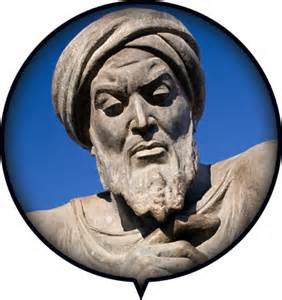
\includegraphics[width=1.1in]{AlKhwartzmi.jpg}
	\caption{\tiny Muhammad ibn Musa al-Khwarizmi (C. 780---850), a Persian scholar, formerly Latinized as Algoritmi}
    \end{figure}
	\begin{itemize}
		\item In the twelfth century, latin translations of his work on the Indian-Arabic numerals introduced the decimal positional number system to the western world. 
	\end{itemize}
}

\frame{
	\frametitle{Al-Khwarizmi`s contributions} 
			\begin{itemize}	
		\item 		 Al-Khwarizmi`s {\it The Compendious Book on Calculation by Completion and Balancing} presented the first systematic solution of \textcolor{red}{\bf linear} and \textcolor{red}{\bf quadratic equations} in Arabic. 
		\item Two words: 
			\begin{itemize}
				\item  \textcolor{red}{\bf Algebra}:  from Arabic ``al-jabr" meaning ``reunion of broken parts" --- one of the two operations he used to solve equations
				\item \textcolor{red}{\bf Algorithm}: a step-by-step set of operations to get solution to a problem 
			\end{itemize}
		\end{itemize}		
}

\frame{
%\frametitle{Algorithm}

\begin{block}{}
 
 {\bf Algorithm design: the art of computer programming }
\end{block}

    \begin{figure}
        \centering
        
\includegraphics[width=0.4\textwidth]{L1-The-Art.jpg}
    \end{figure}
}

\frame{
\frametitle{V. Vazirani said: }

\begin{block}{}
{\it  Our philosophy on the design and exposition of algorithms is nicely illustrated by the following analogy with an aspect of Michelangelos's art:  A major part of his effort involved looking for interesting pieces of stone in the quarry and staring at them for long hours \textcolor{red}{\bf to determine the form they naturally wanted to take}. The chisel work exposed, in a minimal manner, this form. 
}
\end{block}
    \begin{figure}
        \centering
        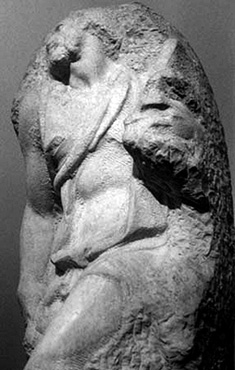
\includegraphics[width=2in]{L1-unfinished.jpg}
    \end{figure}
}

\frame{
\frametitle{V. Vazirani said:  $cont'd$ }

\begin{block}{}
{\it By analogy, we would like to start with a clean, simply stated problem. Most of the algorithm design effort actually goes into \textcolor{red}{\bf understanding the algorithmically relevant combinatorial structure of the problem}.  The algorithm exploits this structure in a minimal manner.....  with emphasis on stating the structure offered by the problems, and keeping the algorithms minimal.  }
\end{block}

(See extra slides.)
}

%  \frame {
%  \frametitle{A first problem: Regular expression matching problem}
%  Contributed by Yanbing Liu, Security lab at ICT. \\
%  (see extra slides.)
%  }
 
% \frame {
% \frametitle{A first problem: Regular expression matching problem}
% \begin{itemize}
%  \item Key observation: solution=vector;
%  \item Solution space size: $O(\prod_{i=1}^n \mid S_i \mid)$ %$O(prod_{i=1}^n S_i)$
%  \item Brute-force: $O(\prod_{i=1}^n \mid S_i \mid)$ time. 
% \end{itemize}
% 
% \begin{figure}
%         \centering
%         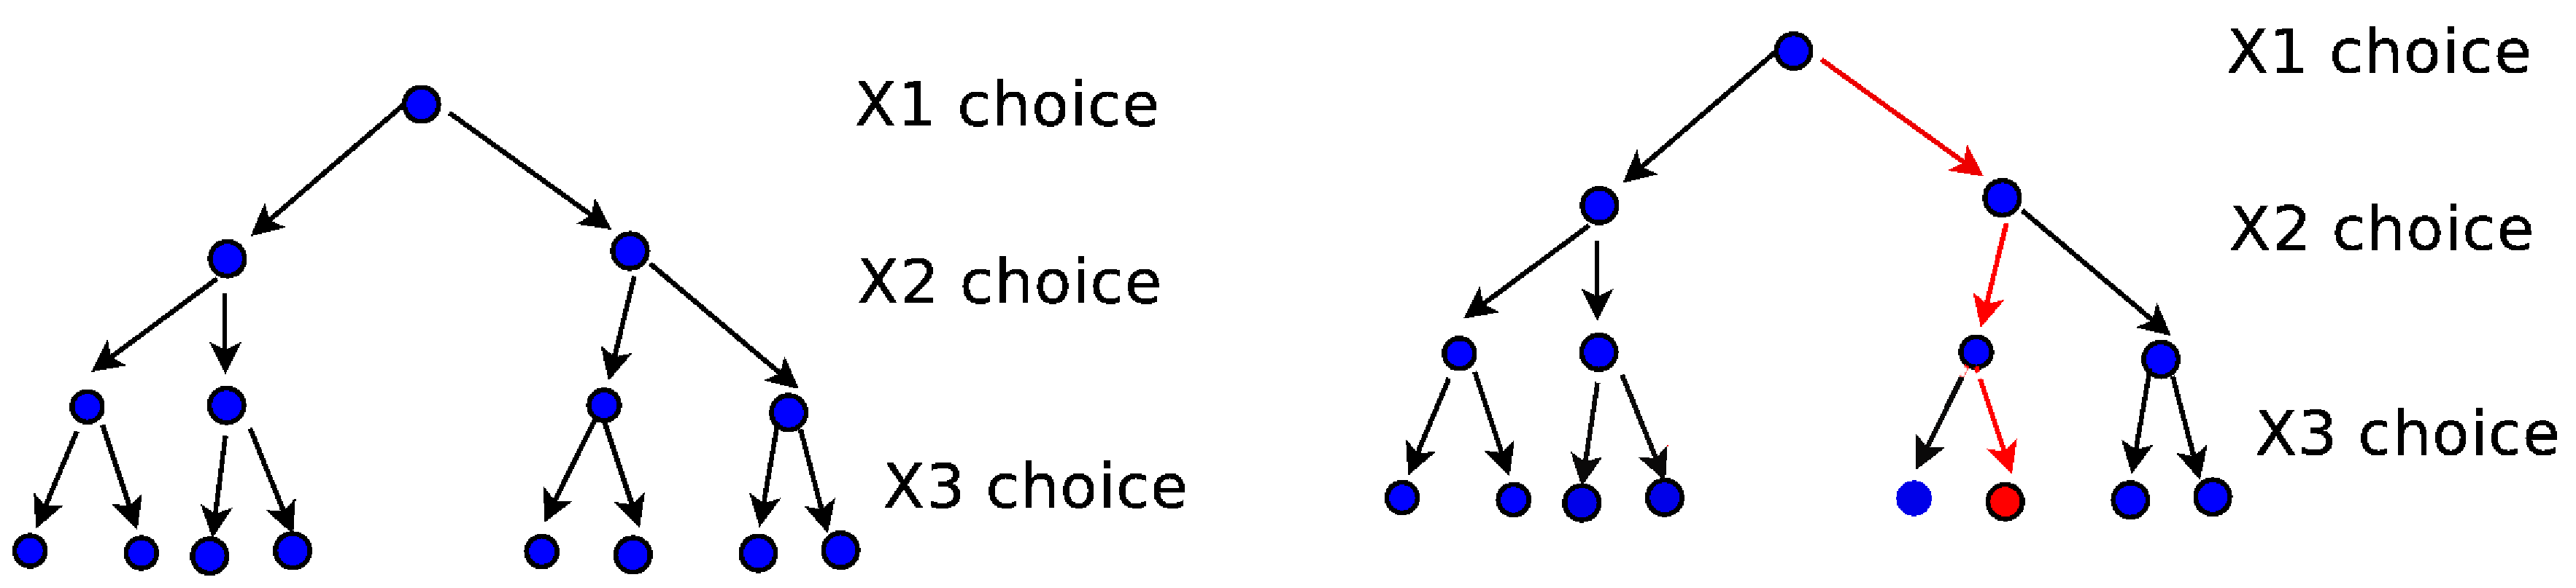
\includegraphics[width=4in]{L1-regularexpressionsearchspace.eps}
% \end{figure}
% }
% 
% 
% \frame {
% \frametitle{A first problem: Regular expression matching problem  $(cont'd)$ }
% \begin{itemize}
%  \item 
% Key observation: solution=vector=path; solution can be decomposed. \\
% \item Key idea: run BFS to check whether the final nodes are reachable; or dynamic programming;
% \item Time-complexity:  $O(4*n)$ \\
% \end{itemize}
% 
% \begin{figure}
%         \centering
%         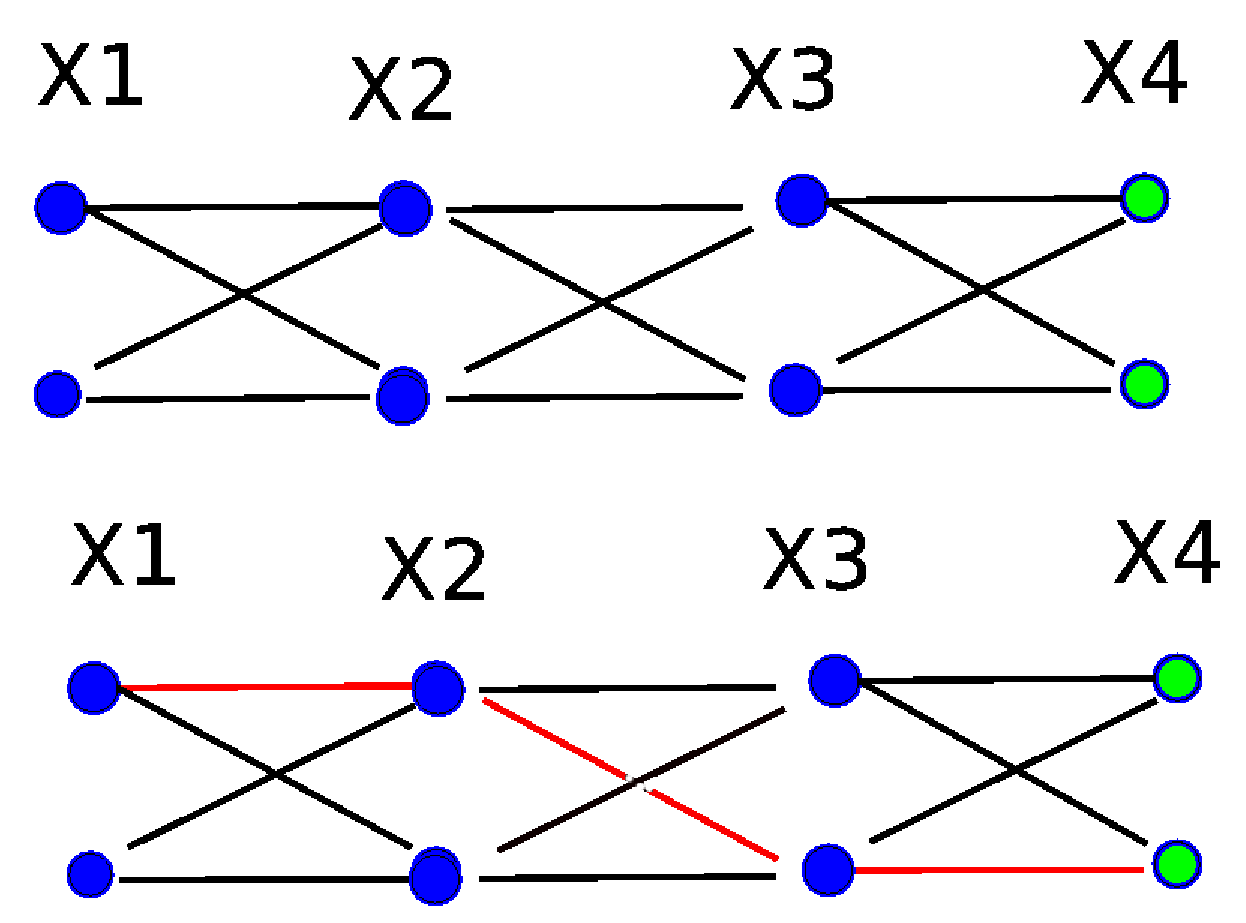
\includegraphics[width=2in]{L1-regularexpressionalgo.eps}
% \end{figure}
% 
%}

\frame{
	\frametitle{Basic algorithmic strategies}
	\begin{itemize}
		\item \textcolor{red}{\bf {\sc Divide-and-conquer}}: Let's start from the ``smallest" problem first, and investigate whether a large problem can \textcolor{blue}{\bf reduce to smaller  subproblems}.  
		\item \textcolor{red}{\bf {\sc Improvement}}: Let's start from  \textcolor{blue}{\bf an initial complete solution}, and try to improve it step by step.  
		\item \textcolor{red}{\bf  {\sc  ``Intelligent" Enumeration}}: Consider an optimization problem. If the solution can be constructed step by step, we might enumerate  \textcolor{blue}{\bf all possible complete solutions} by constructing a \textcolor{blue}{\bf partial solution tree}. Due to the huge size of the search tree, some techniques should be employed to prune it.  
		\end{itemize}
}

\frame {
\begin{block}{}
 
 {\bf The first example: calculating the greatest common divisor  ({\bf gcd})}
\end{block}

} 




\frame {
 \frametitle{The first problem: calculating {\bf gcd} }
 \begin{definition}[$\gcd$]
 	The greatest common divisor of two integers $a$ and $b$, when at least one of them is not zero, is the largest positive integer that divides the numbers without a remainder.
 \end{definition}
 \begin{itemize}
\item
	Example: 
 \begin{itemize}
\item The divisors of 54 are: $1, 2, 3, 6, 9, 18, 27, 54$  
\item The divisors of 24 are: $1, 2, 3, 4, 6, 8, 12, 24$ 
\item Thus, $\gcd(54,24) = 6$. 
 \end{itemize}
 \end{itemize}
 }



\frame {
 \frametitle{The first problem: calculating {\bf gcd} }
 
 \begin{block}{}
  {\bf INPUT: } two $n$-bits numbers $a$, and $b$ ($a\geq b$)\\
  {\bf OUTPUT: } $\gcd(a, b)$
  \end{block}

 \begin{itemize}
 	\item Observation: the problem size can be measured by using $n$; 
	\item Let's start from the ``smallest'' instance: $\gcd( 1, 0) = 1$; 
	\item But how to efficiently solve a ``larger'' instance, say $\gcd( 1949,  101)$?
  \end{itemize}
 }
 
\frame {
\frametitle{Euclidean algorithm } 
 
\begin{figure}
\begin{tikzpicture}[scale=1.1, auto,swap]

    \draw[fill=green!10, rounded corners] (0, 1)  -- (0,0) -- (5, 0) -- (5, 5) -- (0, 5) -- (0, 1); 
            
    \foreach \pos/ \name / \label in {{(2.5,0.5)/gcd01/gcd(1,0)}} 
        \node[smallvertex,fill=red] (\name) at \pos{};
    \foreach \pos/ \name / \label in {{(2.5 + 0.1,0.5)/gcd01/\gcd(1,0)}} 
	   \node[right] at \pos {$\label$}; 

    \foreach \pos/ \name / \label in {{(2.5,4.5)/gcd1949/gcd(1,0)}} 
        \node[smallvertex,fill=blue!20] (\name) at \pos{};
    \foreach \pos/ \name / \label in {{(2.5 + 0.1,4.5)/gcd01/\gcd(1949,101)}} 
	   \node[right] at \pos {$\label$}; 


     
    % Connect vertices with edges and draw weights
%    \foreach \source/ \dest/\weight in {m/w/{}, m'/w'/{} }
%        \path[undirectededge] (\source) -- node[weight] {$\weight$} (\dest);
%       \draw[dashed, ->] (0,0) arc  (120:60:2);

   \node[above] at (2.5, 5.2 ) {Problem instances}; 
   
   
   

       \end{tikzpicture}

\end{figure}
 \begin{itemize}
	\item Observation: a large problem can reduce to a smaller subproblem: 
 	\item $\gcd( 1949, 101) = \gcd( 101, 1949 \mod 101 ) = \gcd( 101, 30)$ \footnote{The Euclidean algorithm was probably invented centuries before Euclid by Hippasus \cite{Xiangwuyi}.}
	
 \end{itemize}
}


\frame {
\frametitle{Strategy: reduce to ``smaller" problems} 
 
\begin{figure}
\begin{tikzpicture}[scale=1.1, auto,swap]

   \draw[fill=green!10, rounded corners] (0, 1)  -- (0,0) -- (5, 0) -- (5, 5) -- (0, 5) -- (0, 1); 

        
    \foreach \pos/ \name / \label in {{(2.5,0.5)/gcd01/gcd(1,0)}} 
        \node[smallvertex,fill=red] (\name) at \pos{};
    \foreach \pos/ \name / \label in {{(2.5 + 0.1,0.5)/gcd01/\gcd(1,0)}} 
	   \node[right] at \pos {$\label$}; 

    \foreach \pos/ \name / \label in {{(2.5,4.5)/gcd1949/gcd(1,0)}} 
        \node[smallvertex,fill=blue!20] (\name) at \pos{};
    \foreach \pos/ \name / \label in {{(2.5 + 0.1,4.5)/gcd01/\gcd(1949,101)}} 
	   \node[right] at \pos {$\label$}; 

    \foreach \pos/ \name / \label in {{(2.5,3.5)/gcd101/gcd(1,0)}} 
        \node[smallvertex,fill=blue!20] (\name) at \pos{};
    \foreach \pos/ \name / \label in {{(2.5 + 0.1, 3.5)/gcd01/\gcd(101, 30)}} 
	   \node[right] at \pos {$\label$}; 

    % Connect vertices with edges and draw weights
    \foreach \source/ \dest/\weight in {gcd1949/gcd101/{}}
        \draw[->] (\source) -- node[weight] {$\weight$} (\dest);
%       \draw[dashed, ->] (0,0) arc  (120:60:2);

   \node[above] at (2.5, 5.2 ) {Problem instances}; 
   
       \end{tikzpicture}
\end{figure}

 \begin{itemize}
 	\item $\gcd( 101, 30) = \gcd( 30, 101 \mod 30 ) = \gcd( 30, 11)$
 \end{itemize}
}


\frame {
\frametitle{Strategy: reduce to "smaller" problems} 
 
\begin{figure}
\begin{tikzpicture}[scale=1.1, auto,swap]

   \draw[fill=green!10, rounded corners] (0, 1)  -- (0,0) -- (5, 0) -- (5, 5) -- (0, 5) -- (0, 1); 
        
    \foreach \pos/ \name / \label in {{(2.5,0.5)/gcd01/gcd(1,0)}} 
        \node[smallvertex,fill=red] (\name) at \pos{};
    \foreach \pos/ \name / \label in {{(2.5 + 0.1,0.5)/gcd01/\gcd(1,0)}} 
	   \node[right] at \pos {$\label$}; 

    \foreach \pos/ \name / \label in {{(2.5,4.5)/gcd1949/gcd(1,0)}} 
        \node[smallvertex,fill=blue!20] (\name) at \pos{};
    \foreach \pos/ \name / \label in {{(2.5 + 0.1,4.5)/gcd01/\gcd(1949,101)}} 
	   \node[right] at \pos {$\label$}; 

    \foreach \pos/ \name / \label in {{(2.5,3.5)/gcd101/gcd(1,0)}} 
        \node[smallvertex,fill=blue!20] (\name) at \pos{};
    \foreach \pos/ \name / \label in {{(2.5 + 0.1, 3.5)/gcd01/\gcd(101, 30)}} 
	   \node[right] at \pos {$\label$}; 

    \foreach \pos/ \name / \label in {{(2.5,2.5)/gcd30/gcd(1,0)}} 
        \node[smallvertex,fill=blue!20] (\name) at \pos{};
    \foreach \pos/ \name / \label in {{(2.5 + 0.1, 2.5)/gcd01/\gcd(30, 11)}} 
	   \node[right] at \pos {$\label$}; 


    % Connect vertices with edges and draw weights
    \foreach \source/ \dest/\weight in {gcd1949/gcd101/{},gcd101/gcd30/{}}
        \draw[->] (\source) -- node[weight] {$\weight$} (\dest);
%       \draw[dashed, ->] (0,0) arc  (120:60:2);

   \node[above] at (2.5, 5.2 ) {Problem instances}; 
   
       \end{tikzpicture}
\end{figure}

 \begin{itemize}
 	\item $\gcd( 30, 11) = \gcd( 11, 30 \mod 11 ) = \gcd( 11, 8)$
 \end{itemize}
}

\frame {
\frametitle{Strategy: reduce to "smaller" problems} 
 
\begin{figure}
\begin{tikzpicture}[scale=1.1, auto,swap]

   \draw[fill=green!10, rounded corners] (0, 1)  -- (0,0) -- (5, 0) -- (5, 5) -- (0, 5) -- (0, 1); 
        
    \foreach \pos/ \name / \label in {{(2.5,0.5)/gcd01/gcd(1,0)}} 
        \node[smallvertex,fill=red] (\name) at \pos{};
    \foreach \pos/ \name / \label in {{(2.5 + 0.1,0.5)/gcd01/\gcd(1,0)}} 
	   \node[right] at \pos {$\label$}; 

    \foreach \pos/ \name / \label in {{(2.5,4.5)/gcd1949/gcd(1,0)}} 
        \node[smallvertex,fill=blue!20] (\name) at \pos{};
    \foreach \pos/ \name / \label in {{(2.5 + 0.1,4.5)/gcd01/\gcd(1949,101)}} 
	   \node[right] at \pos {$\label$}; 

    \foreach \pos/ \name / \label in {{(2.5,3.5)/gcd101/gcd(1,0)}} 
        \node[smallvertex,fill=blue!20] (\name) at \pos{};
    \foreach \pos/ \name / \label in {{(2.5 + 0.1, 3.5)/gcd01/\gcd(101, 30)}} 
	   \node[right] at \pos {$\label$}; 

    \foreach \pos/ \name / \label in {{(2.5,2.5)/gcd30/gcd(1,0)}} 
        \node[smallvertex,fill=blue!20] (\name) at \pos{};
    \foreach \pos/ \name / \label in {{(2.5 + 0.1, 2.5)/gcd01/\gcd(30, 11)}} 
	   \node[right] at \pos {$\label$}; 


    % Connect vertices with edges and draw weights
    \foreach \source/ \dest/\weight in {gcd1949/gcd101/{},gcd101/gcd30/{}}
        \draw[->] (\source) -- node[weight] {$\weight$} (\dest);
%       \draw[dashed, ->] (0,0) arc  (120:60:2);

    \foreach \source/ \dest/\weight in {gcd30/gcd01/{}}
        \draw[dashed, ->] (\source) -- node[weight] {$\weight$} (\dest);
%       \draw[dashed, ->] (0,0) arc  (120:60:2);

   \node[above] at (2.5, 5.2 ) {Problem instances}; 
       \end{tikzpicture}
\end{figure}

 \begin{itemize}
 	\item $\gcd( 30, 11) =  \gcd( 11, 8) = \gcd(8, 3) = \gcd( 3, 2) = \gcd( 2, 1) = \gcd( 1, 0) = 1  $
 \end{itemize}
}

\frame {
\frametitle{Sub-instance relationship graph} 
 
\begin{figure}
\begin{tikzpicture}[scale=1.1, auto,swap]

   \draw[fill=green!10, rounded corners] (0, 1)  -- (0,0) -- (5, 0) -- (5, 5) -- (0, 5) -- (0, 1); 
        
    \foreach \pos/ \name / \label in {{(2.5,0.5)/gcd01/gcd(1,0)}} 
        \node[smallvertex,fill=red] (\name) at \pos{};
    \foreach \pos/ \name / \label in {{(2.5 + 0.1,0.5)/gcd01/\gcd(1,0)}} 
	   \node[right] at \pos {$\label$}; 

    \foreach \pos/ \name / \label in {{(2.5,4.5)/gcd1949/gcd(1,0)}} 
        \node[smallvertex,fill=blue!20] (\name) at \pos{};
    \foreach \pos/ \name / \label in {{(2.5 + 0.1,4.5)/gcd01/\gcd(1949,101)}} 
	   \node[right] at \pos {$\label$}; 

    \foreach \pos/ \name / \label in {{(2.5,3.5)/gcd101/gcd(1,0)}} 
        \node[smallvertex,fill=blue!20] (\name) at \pos{};
    \foreach \pos/ \name / \label in {{(2.5 + 0.1, 3.5)/gcd01/\gcd(101, 30)}} 
	   \node[right] at \pos {$\label$}; 

    \foreach \pos/ \name / \label in {{(2.5,2.5)/gcd30/gcd(1,0)}} 
        \node[smallvertex,fill=blue!20] (\name) at \pos{};
    \foreach \pos/ \name / \label in {{(2.5 + 0.1, 2.5)/gcd01/\gcd(30, 11)}} 
	   \node[right] at \pos {$\label$}; 


    % Connect vertices with edges and draw weights
    \foreach \source/ \dest/\weight in {gcd1949/gcd101/{},gcd101/gcd30/{}}
        \draw[->] (\source) -- node[weight] {$\weight$} (\dest);
%       \draw[dashed, ->] (0,0) arc  (120:60:2);

    \foreach \source/ \dest/\weight in {gcd30/gcd01/{}}
        \draw[dashed, ->] (\source) -- node[weight] {$\weight$} (\dest);
%       \draw[dashed, ->] (0,0) arc  (120:60:2);

   \node[above] at (2.5, 5.2 ) {Problem instances}; 
       \end{tikzpicture}
\end{figure}

 \begin{itemize}
 	\item Node: subproblems 
	\item Edge: reduction relationship 
 \end{itemize}
}

\frame {
\frametitle{Euclid algorithm } 


{\bf function} {\sc Euclid}$(a,b)$
\begin{algorithmic}[1]
%\STATE { /* $a$ and $b$ are integers, and $a \geq b \geq 0$ */ }  
\IF{ $ b = 0 $ }  
	\RETURN $a$; 
\ENDIF
\RETURN{{\sc Euclid}$(b, a\mod b)$}; 
\end{algorithmic}
} 

\frame {
\frametitle{Time complexity analysis } 

\begin{Theorem}
Suppose $a$ is a $n$-bit integer. Euclid($a$, $b$) ends in $O(n^3)$ time. 
\end{Theorem}
\begin{Proof}
	\begin{itemize}
		\item There are at most $2n$ recursive calling. 
			\begin{itemize}
				\item Note that $ a \mod b < \frac{a}{2}$. 
				\item After two rounds of recursive calling, both $a$ and $b$ shrink at least a half size. 
			\end{itemize}
		\item At each recursive calling, the $\mod$ operation costs $O(n^2)$ time. 
	\end{itemize}
\end{Proof}

} 

\frame{
\begin{block}{}
{\bf The second example: traveling salesman problem (TSP)}
\end{block}

}



\frame{
	\frametitle{TSP: a concrete example } 
	
	\begin{figure}
	\begin{minipage}{1in}
        	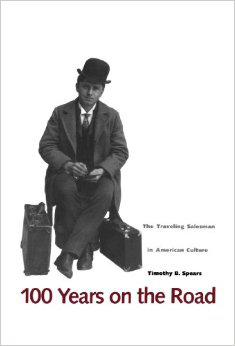
\includegraphics[width=\textwidth]{TSP-100years.png}
	\end{minipage}
	\begin{minipage}{1.5in}
        	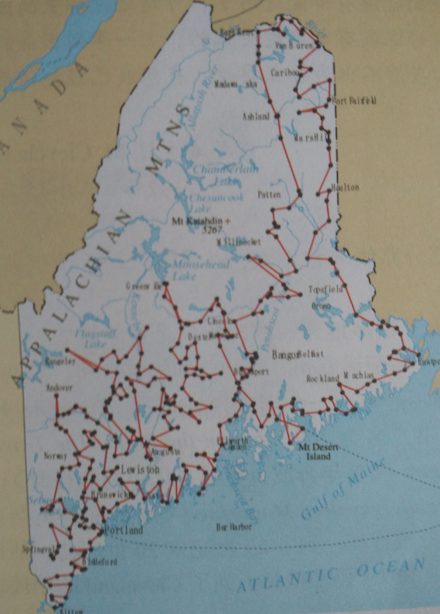
\includegraphics[width=\textwidth]{TSP-350.png}
	\end{minipage}
    \end{figure}
\begin{itemize}
	\item In 1925, H. M. Cleveland, a salesman of the Page seed company, traveled 350 cities to gather order form. 
	\item Of course, the shorter the total distance, the better. 
\end{itemize}
}


\frame{
	\frametitle{How did they do? Pin and wire! } 
	
	\begin{figure}
	\begin{minipage}{2in}
        	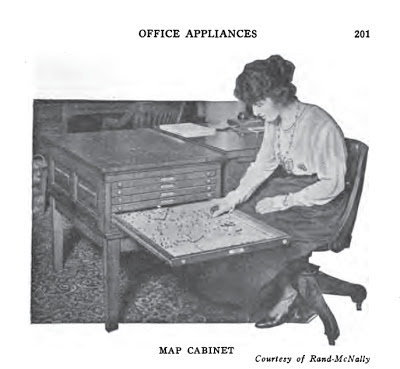
\includegraphics[width=\textwidth]{TSP-Secretary.jpg}
	\end{minipage}
	\begin{minipage}{1.5in}
        	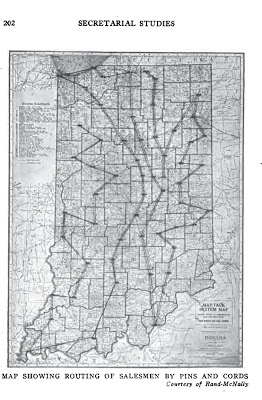
\includegraphics[width=\textwidth]{TSP-Secretary2.jpg}
	\end{minipage}
    \end{figure}
\begin{itemize}
	\item Two pictures excerpted from {\it Secretarial Studies}, 1922. 
\end{itemize}
}



\frame{
	\frametitle{ {\sc Travelling Salesman Problem}  } 

	\begin{block}{}
		{\bf INPUT:  } $n$ cities $V=\{1, 2, ..., n\}$,  and a distance matrix $D$, where $d_{ij}$ $(1\leq i, j \leq n)$ denotes the distance between city $i$ and $j$. \\ 
		{\bf OUTPUT: }  the shortest tour that visits each city exactly once and returns to the origin city. 
	\end{block} 	
	
\begin{figure}
	\begin{tikzpicture}[scale=1, auto,swap]

    \foreach \pos/ \name in {{(0,0)/1},{(0,2)/2}, {(2,2)/3}, {(2,0)/4}} 
        \node[smallvertex,fill=blue!20] (\name) at \pos{$\name$};

     
    % Connect vertices with edges and draw weights
    \foreach \source/ \dest/\weight in {2/1/{1},   1/4/{3}, 3/2/{5}, 4/3/{3}}
        \path[undirectededge] (\source) -- node[weight] {$\weight$} (\dest);
    \foreach \source/ \dest/\weight in  {3/1/{}, 4/2/{}}
        \path[undirectededge] (\source) -- node[weight] {$\weight$} (\dest);
     
     \node at (0.6, 0.3) {\small $8$};   
     \node at (0.6, 1.7) {\small $7$};   
        
     \end{tikzpicture}
\end{figure}
%$\#$Tours:  $6$
\begin{itemize}
	\begin{small}
		\item Tour 1: $1\rightarrow 2 \rightarrow 3 \rightarrow 4 \rightarrow 1$ (distance: 12)
		\item Tour 2: $1\rightarrow 2 \rightarrow 4 \rightarrow 3 \rightarrow 1$ (distance: 19)
		\item Tour 3: $1\rightarrow 3 \rightarrow 2 \rightarrow 4 \rightarrow 1$ (distance: 23)
		\item Tour 4: $1\rightarrow 3 \rightarrow 4 \rightarrow 2 \rightarrow 1$ (distance: 19)
		\item Tour 5: $1\rightarrow 4 \rightarrow 2 \rightarrow 3 \rightarrow 1$ (distance: 23)
		\item Tour 6: $1\rightarrow 4 \rightarrow 3 \rightarrow 2 \rightarrow 1$ (distance: 12)
	\end{small}
\end{itemize}

}


\frame{
\begin{block}{}
{\bf Trial 1: Divide and conquer}
\end{block}
}



\frame{
	\frametitle{Decompose the original problem into subproblems} 

	
\begin{figure}
	\begin{tikzpicture}[scale=1, auto,swap]

\def\dx{0};
 
     \foreach \pos/ \name in {{(-2 + \dx ,0)/a},{(2+ \dx ,0)/b}, {(-1+ \dx ,1.6)/e}, {(1+ \dx ,1.6)/c}} 
        \node[smallvertex,fill=blue!20] (\name) at \pos{$\name$};
     
    \foreach \source/ \dest/\weight in {a/b/{3},   a/c/{4}, e/a/{7}, b/c/{4}, e/b/{3}, c/e/{8}}
        \path[undirectededge] (\source) -- node[weight] {\small $\weight$} (\dest);
         
    \foreach \source/ \dest/\weight in {a/b/,   b/c/}
        \path[undirectededge, black] (\source) -- node[weight] {$\weight$} (\dest);

    \foreach \source/ \dest/\weight in {a/b/,   e/c/}
        \path[undirectededge, black] (\source) -- node[weight] {$\weight$} (\dest);

    \foreach \source/ \dest/\weight in {b/e/,  a/c/, c/e/, a/b/}
        \path[undirectededge, red] (\source) -- node[weight] {$\weight$} (\dest);

 
 \def\dx{-6};
 
     \foreach \pos/ \name in {{(-2 + \dx ,0)/a},{(2+ \dx ,0)/b}, {(-1+ \dx ,1.6)/e}, {(1+ \dx ,1.6)/c}, {(0+ \dx ,3.2)/d}} 
        \node[smallvertex,fill=blue!20] (\name) at \pos{$\name$};
     
    % Connect vertices with edges and draw weights
     %   \foreach \source/ \dest/\weight in {a/b/{3},   c/a/{4}, e/a/{7}, a/d/{2}, b/c/{4}, b/d/{6}, e/b/{3}, c/d/{5}, c/e/{8}, d/e/{6}}
    \foreach \source/ \dest/\weight in {a/b/{3},   a/c/{4}, e/a/{7}, b/c/{4}, e/b/{3}, c/d/{5}, c/e/{8}, d/e/{6}}
        \path[undirectededge] (\source) -- node[weight] {\small $\weight$} (\dest);
         
    \draw[thick] (a)   to [out=140, in=180] node[above] {2} (d);   
        \draw[thick] (b)   to [out=40, in=0] node[above] {6} (d);   

    \foreach \source/ \dest/\weight in {b/e/,   b/c/,   d/e/, a/c/}
        \path[undirectededge, blue] (\source) -- node[weight] {$\weight$} (\dest);

   \draw[thick, blue] (a)   to [out=140, in=180] node[above] {2} (d);   

 \end{tikzpicture}
\end{figure}

\begin{itemize}

	\item Note that it is not easy to obtain the optimal solution to the original problem (e.g., tour in blue) through the optimal solution to subproblem (e.g., tour in red). 
	
\end{itemize}

}


\frame{
	\frametitle{Consider a tightly-related problem }

	\begin{itemize}
%		\item Note the solution is a tour of the $n$ cities. 
		\item  Let's consider a tightly-related problem: calculating $M(s, S, x)$, the minimum distance, starting from city $s$, visiting each city in $S$ once and exactly once, and ending at city $x$. 
		 \item It is easy to decompose this problem into subproblems, and the original problem could be easily solved if $M(s, S, x)$ were determined for all subset $S\subseteq V$ and $e\in V$.
		
		\begin{figure}
	\begin{tikzpicture}[scale=1, auto,swap]

    \foreach \pos/ \name in {{(0,0)/1},{(0,1.5)/2}, {(1.5,1.5)/3}, {(1.5,0)/4}} 
        \node[smallvertex,fill=blue!20] (\name) at \pos{$\name$};

     
    % Connect vertices with edges and draw weights
    \foreach \source/ \dest/\weight in {2/1/{1},   1/4/{3}, 3/2/{5}, 4/3/{3}}
        \path[undirectededge] (\source) -- node[weight] {$\weight$} (\dest);
    \foreach \source/ \dest/\weight in  {3/1/{}, 4/2/{}}
        \path[undirectededge] (\source) -- node[weight] {$\weight$} (\dest);
     
     \node at (0.6, 0.3) {\small $8$};   
     \node at (0.6, 1.2) {\small $7$};   
          
	\end{tikzpicture}
\end{figure}
		
		\item For example, since there are 3 cases of the city from which we return to $1$, the shortest tour can be calculated as: 
\[ 
\begin{array}{lll}
\min\{ & d_{2,1} + M(1, \{ 3, 4\}, 2), \\ 
              & d_{3,1} + M(1, \{2, 4\}, 3 ), \\ 
              & d_{4,1} + M(1, \{ 2, 3\}, 4 )   \}
\end{array}            
\]
	\end{itemize}

}



\frame{
	\frametitle{Consider the smallest instance of $M(s, S, x)$}


	\begin{itemize}
		\item It is trivial to calculate $M(s, S, x)$ when $S$ consists of only 1 city. 
\begin{figure}
	\begin{tikzpicture}[scale=1, auto,swap]

    \foreach \pos/ \name in {{(0,0)/1},{(0,1.5)/2}, {(1.8,1.5)/3}} 
        \node[smallvertex,fill=blue!20] (\name) at \pos{$\name$};

    % Connect vertices with edges and draw weights
    \foreach \source/ \dest/\weight in {2/1/{1},   3/2/{5}}
        \path[undirectededge] (\source) -- node[weight] {$\weight$} (\dest);
    \foreach \source/ \dest/\weight in  {3/1/{8}}
        \path[undirectededge] (\source) -- node[weight] {$\weight$} (\dest);

    \foreach \source/ \dest/\weight in {2/1/{},   3/2/{}}
        \path[undirectededge, red] (\source) -- node[weight] {$\weight$} (\dest);
        
   \def\dx{5};
   
    \foreach \pos/ \name in {{(0+\dx,0)/1},{(0+\dx,1.5)/2}, {(1.8+\dx,1.5)/3}} 
        \node[smallvertex,fill=blue!20] (\name) at \pos{$\name$};

    % Connect vertices with edges and draw weights
    \foreach \source/ \dest/\weight in {2/1/{1},   3/2/{5}}
        \path[undirectededge] (\source) -- node[weight] {$\weight$} (\dest);
    \foreach \source/ \dest/\weight in  {3/1/{8}}
        \path[undirectededge] (\source) -- node[weight] {$\weight$} (\dest);

    \foreach \source/ \dest/\weight in {2/3/{},   3/1/{}}
        \path[undirectededge, red] (\source) -- node[weight] {$\weight$} (\dest);
        
        
        \node[] at (0, -0.5) {\small $M(1, \{ 2\}, 3) = d_{12} + d_{23}$}; 
        \node[] at (0+\dx, -0.5) {\small $M(1, \{  3\}, 2) = d_{13} + d_{32}$}; 
                
	\end{tikzpicture}


\end{figure}


%		\item $M( \{ 2\}, 3) = d_{12} + d_{23}$ $\qquad$ $M( \{  3\}, 2) = d_{13} + d_{32}$
		\item But how to solve a larger problem, say $M(1, \{2, 3\}, 4)$?
	\end{itemize}
}

%\frame{
%	\frametitle{Sub-instance relationship graph}
%	\begin{figure}
%\begin{tikzpicture}[scale=1.1, auto,swap]
%
%   \draw[fill=green!10, rounded corners] (0, 1)  -- (0,0) -- (5, 0) -- (5, 5) -- (0, 5) -- (0, 1); 
%        
%    \foreach \pos/ \name / \label in {{(2.5,3.5)/D1234/}} 
%        \node[smallvertex,fill=blue!20] (\name) at \pos{};
%    \foreach \pos/ \name / \label in {{(2.5 + 0.1, 3.5)/D1234/M(\{2,3\}, 4)}} 
%	   \node[right] at \pos {\small $\label$}; 
%
%    \foreach \pos/ \name / \label in {{(2,1.5)/D1232/}} 
%        \node[smallvertex,fill=red] (\name) at \pos{};
%    \foreach \pos/ \name / \label in {{(2 - 0.1, 1.5)/D1232/M(\{3\}, 2) }} 
%	   \node[left] at \pos {\small $\label$}; 
%
%    \foreach \pos/ \name / \label in {{(3,1.5)/D1233/}} 
%        \node[smallvertex,fill=red] (\name) at \pos{};
%    \foreach \pos/ \name / \label in {{(3 + 0.1, 1.5)/D1233/M(\{2\}, 3) }} 
%	   \node[right] at \pos {\small $\label$}; 
%
%
%   \node[above] at (2.5, 5.2 ) {Problem instances}; 
%       \end{tikzpicture}
%\end{figure}
%
%}



\frame{
	\frametitle{Divide a large problem into smaller problems }

\begin{figure}
	\begin{tikzpicture}[scale=1, auto,swap]

    \foreach \pos/ \name in {{(0,0)/1},{(0,1.8)/2}, {(1.8,1.8)/3}, {(1.8,0)/4}} 
        \node[smallvertex,fill=blue!20] (\name) at \pos{$\name$};

     
    % Connect vertices with edges and draw weights
    \foreach \source/ \dest/\weight in {2/1/{1},   1/4/{3}, 3/2/{5}, 4/3/{3}}
        \path[undirectededge] (\source) -- node[weight] {$\weight$} (\dest);
    \foreach \source/ \dest/\weight in  {3/1/{}, 4/2/{}}
        \path[undirectededge] (\source) -- node[weight] {$\weight$} (\dest);
     
     \node at (0.6, 0.3) {\small $8$};   
     \node at (0.6, 1.5) {\small $7$};   
        
%red 	
    \foreach \source/ \dest/\weight in  {1/2/{}, 2/3/{}, 4/3/{}}
        \path[undirectededge,red] (\source) -- node[weight] {$\weight$} (\dest);




    \foreach \pos/ \name in {{(4,0)/1},{(4,1.8)/2}, {(5.8,1.8)/3}, {(5.8,0)/4}} 
        \node[smallvertex,fill=blue!20] (\name) at \pos{$\name$};

     
    % Connect vertices with edges and draw weights
    \foreach \source/ \dest/\weight in {2/1/{1},   1/4/{3}, 3/2/{5}, 4/3/{3}}
        \path[undirectededge] (\source) -- node[weight] {$\weight$} (\dest);
    \foreach \source/ \dest/\weight in  {3/1/{}, 4/2/{}}
        \path[undirectededge] (\source) -- node[weight] {$\weight$} (\dest);
     
     \node at (4+0.6, 0.3) {\small $8$};   
     \node at (4+0.6, 1.5) {\small $7$};   
        
%red 	
    \foreach \source/ \dest/\weight in  {1/3/{}, 2/3/{}, 4/2/{}}
        \path[undirectededge,red] (\source) -- node[weight] {$\weight$} (\dest);

        
	\end{tikzpicture}
\end{figure}

	\begin{itemize}
		\item $M(1, \{2, 3\}, 4) = \min\{ d_{34} + M(1, \{2\}, 3), d_{24} + M(1, \{ 3\}, 2)  \} $
	\end{itemize}
}

\frame{
	\frametitle{Sub-instance relationship graph }
	\begin{figure}
\begin{tikzpicture}[scale=1.1, auto,swap]

   \draw[fill=green!10, rounded corners] (0, 1)  -- (0,0) -- (5, 0) -- (5, 5) -- (0, 5) -- (0, 1); 
        
    \foreach \pos/ \name / \label in {{(2.5,3.5)/D1234/}} 
        \node[smallvertex,fill=blue!20] (\name) at \pos{};
    \foreach \pos/ \name / \label in {{(2.5 + 0.1, 3.5)/D1234/M(1,\{2,3\}, 4)}} 
	   \node[right] at \pos {\small $\label$}; 

    \foreach \pos/ \name / \label in {{(2,1.5)/D1232/}} 
        \node[smallvertex,fill=red] (\name) at \pos{};
    \foreach \pos/ \name / \label in {{(2 - 0.1, 1.5)/D1232/M(1,\{3\}, 2) }} 
	   \node[left] at \pos {\small $\label$}; 

    \foreach \pos/ \name / \label in {{(3,1.5)/D1233/}} 
        \node[smallvertex,fill=red] (\name) at \pos{};
    \foreach \pos/ \name / \label in {{(3 + 0.1, 1.5)/D1233/M(1,\{2\}, 3) }} 
	   \node[right] at \pos {\small $\label$}; 

    % Connect vertices with edges and draw weights
    \foreach \source/ \dest/\weight in {D1234/D1232/{},D1234/D1233/{}}
        \draw[->] (\source) -- node[weight] {$\weight$} (\dest);
%       \draw[dashed, ->] (0,0) arc  (120:60:2);

   \node[above] at (2.5, 5.2 ) {Problem instances}; 
       \end{tikzpicture}
\end{figure}

\begin{itemize}
	\item A large problem  can be reduced into smaller subproblems. 
\end{itemize}


}

\frame{
	\frametitle{ Held-Karp algorithm [1962]} 

{\bf function} {\sc TSP}$(D)$
\begin{algorithmic}[1]
\RETURN{$\min_{e \in V, e \neq s}{\sc M}(s, V - \{e\}, e) + d_{es}$}; 
\end{algorithmic}
\quad \\
\quad \\
{\bf function} {\sc M}$(s, S, x)$
\begin{algorithmic}[1]
\IF{ $ S = \{v\}$ }
	\STATE {\sc M}$(s, S, x) = d_{sv} + d_{vx}$; 
	\RETURN{{\sc M}$(s, S, x)$}; 
\ENDIF
\RETURN{$\min_{i \in S,\ i \neq x}${\sc M}$(s, S - \{i\}, i) + d_{xi}$}; 
\end{algorithmic}

}

\frame{
	\frametitle{An example } 
	
\begin{table}[H]
	\centering
%\caption{\fangsong 对图\ref{MSE}$(b)$所示TSP实例计算出的$M(a, S, x)$表格}\label{MsSxExample}
	\begin{small}
	\begin{tabular}{crrr}
		\hline 
		 & \multicolumn{3}{c}{ $x$} \\ 
		         \cline{2-4} 
		{ $S$} & $b$ & $c$ & $d$  \\         
		\hline 
		$\{b\}$ &   -   &  7   & 6       \\ 
		$\{c\}$ &   8   &  -   &   12       \\ 
		$\{d\}$ &  10   &  15   &   -     \\ 
		$\{b, c\}$ &  -   & -   &  15       \\ 
		$\{b, d\}$ &  -   & 14   &  -    \\ 
		$\{c, d\}$ &  15   & -   &  -    \\ 
		\hline
	\end{tabular}
	\end{small}
\end{table}


\begin{itemize}
	\item Time complexity: $O( 2^n n^2)$. 
\end{itemize}
	
} 
	


\frame{
\begin{block}{}
{\bf Trial 2: Improvement strategy  }
\end{block}
}

\frame{
	\frametitle{Solution space  }

\begin{figure}
        \centering
        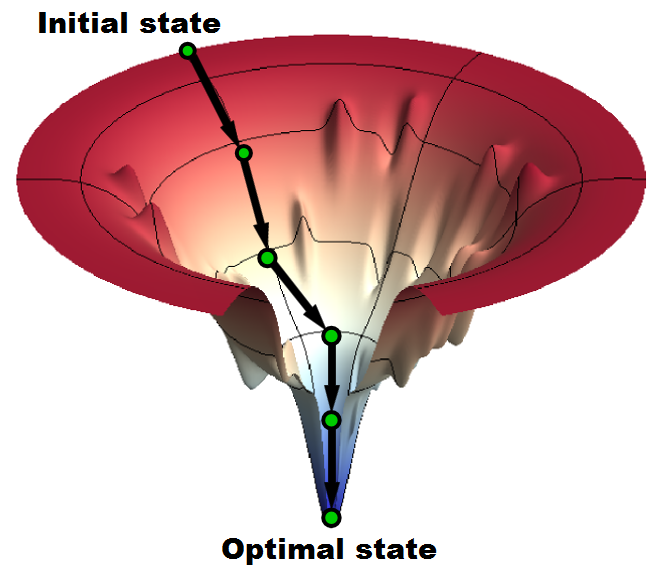
\includegraphics[width=1.8in]{Landscape.png}
%	\caption{\tiny Muhammad ibn Musa al-Khwarizmi (C. 780---850), a Persian scholar, formerly Latinized as Algoritmi}
\end{figure}
\begin{itemize}
	\item Landscape of solution space: 
 	\begin{itemize}
		\item Node: a complete solution. Each node is associated with an objective function value. 
		\item Edge: if two nodes are neighboors, an edge is added to connect them. Here "neighbours" refers to two nodes with small difference. 
	\end{itemize}
	\item Improvement strategy:  start from a rough complete solution, and try to improve it step by step. 
\end{itemize}

    
} 

\frame{
	\frametitle{ {\sc Improvement} strategy }

\begin{figure}
	\begin{tikzpicture}[scale=1, auto,swap]

    \foreach \pos/ \name in {{(0,0)/1},{(0,2)/2}, {(2,2)/3}, {(2,0)/4}} 
        \node[smallvertex,fill=blue!20] (\name) at \pos{$\name$};

     
    % Connect vertices with edges and draw weights
    \foreach \source/ \dest/\weight in {2/1/{1},   1/4/{3}, 3/2/{5}, 4/3/{3}}
        \path[undirectededge] (\source) -- node[weight] {$\weight$} (\dest);
    \foreach \source/ \dest/\weight in  {3/1/{}, 4/2/{}}
        \path[undirectededge] (\source) -- node[weight] {$\weight$} (\dest);
     
     \node at (0+0.6, 0.3) {\small $8$};   
     \node at (0+0.6, 1.7) {\small $7$};   
        
	\end{tikzpicture}
\end{figure}

	\begin{itemize}
		\item Note that a \textcolor{red}{\bf complete solution} can be expressed as a  permutations of the $n$ cities, e.g., $1, 2, 3, 4$.
		\item Let's start from \textcolor{red}{\bf an initial  complete solution}, and try to improve it;
	\end{itemize} 
	
	 
}


\frame{
	\frametitle{ {\sc Improvement} strategy }

%\begin{figure}
%	\begin{tikzpicture}[scale=0.8, auto,swap]
%
%    \foreach \pos/ \name in {{(0,0)/1},{(0,2)/2}, {(2,2)/3}, {(2,0)/4}} 
%        \node[smallvertex,fill=blue!20] (\name) at \pos{$\name$};
%
%     
%    % Connect vertices with edges and draw weights
%    \foreach \source/ \dest/\weight in {2/1/{1},   1/4/{3}, 3/2/{5}, 4/3/{3}}
%        \path[undirectededge] (\source) -- node[weight] {$\weight$} (\dest);
%    \foreach \source/ \dest/\weight in  {3/1/{8}, 4/2/{7}}
%        \path[undirectededge] (\source) -- node[weight] {$\weight$} (\dest);
%        
%	\end{tikzpicture}
%\end{figure}


{\bf function} {\sc GenericImprovement($V, D)$}	
\begin{algorithmic}[1]
\STATE Let $s$ be an initial tour; 
\WHILE{{\tt TRUE} }
	\STATE Select a new tour $s'$ from the \textcolor{red}{\bf neighbourhood} of $s$; 
	\IF{$s'$ is shorter than $s$ }  
		\STATE $s = s'$; 
	\ENDIF
	\IF{stopping($s$)}
		\RETURN{$s$}; 
	\ENDIF
\ENDWHILE
\end{algorithmic}
Here, \textcolor{red}{\bf neighbourhood} is introduced to describe how to change an existing tour into a new one;  
	 
}

\frame{
	\frametitle{But how to define neighbourhood of a tour? } 
	\begin{itemize}
		\item 2-opt strategy: if $s'$ and $s$ differ at only two edges (Note: 1-opt is impossible)
	\end{itemize}

\begin{figure}
	\begin{tikzpicture}[scale=1, auto,swap]

    \foreach \pos/ \name in {{(4,0)/1},{(4,2)/2}, {(6,2)/3}, {(6,0)/4}} 
        \node[smallvertex,fill=blue!20] (\name) at \pos{$\name$};
    
    % Connect vertices with edges and draw weights
    \foreach \source/ \dest/\weight in {2/1/{1},   3/4/{3} }
        \path[undirectededge] (\source) -- node[weight] { } (\dest);
    \foreach \source/ \dest/\weight in  {3/1/{8}, 4/2/{7}}
        \path[undirectededge, red] (\source) -- node[weight] { } (\dest);
 
 	\node[] at (1, -0.5) {$s$}; 

 	\node[] at (5, -0.5) {$s'$}; 
   
   \draw[->, blue, line width=2pt] (2.6, 1) -- (3.4, 1);
 
    \foreach \pos/ \name in {{(0,0)/1},{(0,2)/2}, {(2,2)/3}, {(2,0)/4}} 
        \node[smallvertex,fill=blue!20] (\name) at \pos{$\name$};

    
    % Connect vertices with edges and draw weights
    \foreach \source/ \dest/\weight in {2/1/{1},   3/4/{3} }
        \path[undirectededge] (\source) -- node[weight] { } (\dest);
    \foreach \source/ \dest/\weight in  {4/1/{8}, 3/2/{7}}
        \path[undirectededge, red] (\source) -- node[weight] { } (\dest);
        
 
        
	\end{tikzpicture}
\end{figure}
		
}


\frame{
	\frametitle{An example} 
		
\begin{figure}
	\begin{tikzpicture}[scale=1, auto,swap]

    \foreach \pos/ \name in {{(-2,0)/a},{(2,0)/b}, {(-1,1.6)/e}, {(1,1.6)/c}, {(0,3.2)/d}} 
        \node[smallvertex,fill=blue!20] (\name) at \pos{$\name$};
     
    % Connect vertices with edges and draw weights
     %   \foreach \source/ \dest/\weight in {a/b/{3},   c/a/{4}, e/a/{7}, a/d/{2}, b/c/{4}, b/d/{6}, e/b/{3}, c/d/{5}, c/e/{8}, d/e/{6}}
    \foreach \source/ \dest/\weight in {a/b/{3},   a/c/{4}, e/a/{7}, b/c/{4}, e/b/{3}, c/d/{5}, c/e/{8}, d/e/{6}}
        \path[undirectededge] (\source) -- node[weight] {\small $\weight$} (\dest);
         
    \draw[thick] (a)   to [out=140, in=180] node[above] {2} (d);   
        \draw[thick] (b)   to [out=40, in=0] node[above] {6} (d);   
\end{tikzpicture}
\end{figure}


}

\frame{
	\frametitle{Step 1} 

\begin{figure}
	\begin{tikzpicture}[scale=1, auto,swap]

    \foreach \pos/ \name in {{(-2,0)/a},{(2,0)/b}, {(-1,1.6)/e}, {(1,1.6)/c}, {(0,3.2)/d}} 
        \node[smallvertex,fill=blue!20] (\name) at \pos{$\name$};
     
    % Connect vertices with edges and draw weights
     %   \foreach \source/ \dest/\weight in {a/b/{3},   c/a/{4}, e/a/{7}, a/d/{2}, b/c/{4}, b/d/{6}, e/b/{3}, c/d/{5}, c/e/{8}, d/e/{6}}
    \foreach \source/ \dest/\weight in {a/b/{3},   a/c/{4}, e/a/{7}, b/c/{4}, e/b/{3}, c/d/{5}, c/e/{8}, d/e/{6}}
        \path[undirectededge] (\source) -- node[weight] {\small $\weight$} (\dest);
         
    \draw[thick] (a)   to [out=140, in=180] node[above] {2} (d);   
        \draw[thick] (b)   to [out=40, in=0] node[above] {6} (d);   
        
       \foreach \source/ \dest/\weight in {a/b/,   b/c/,  c/d/, d/e/, e/a/}
        \path[undirectededge, blue] (\source) -- node[weight] {$\weight$} (\dest);


\end{tikzpicture}
\end{figure}


\begin{itemize}
	\item 	Initial complete solution $s$:  $a \rightarrow b\rightarrow c\rightarrow  d\rightarrow  e\rightarrow a $  (distance: 25)
\end{itemize}

}


\frame{
	\frametitle{Step 2: a 2-opt operation improves $s \Rightarrow s'$ } 
	
\begin{figure}
	\begin{tikzpicture}[scale=1, auto,swap]

    \foreach \pos/ \name in {{(-2,0)/a},{(2,0)/b}, {(-1,1.6)/e}, {(1,1.6)/c}, {(0,3.2)/d}} 
        \node[smallvertex,fill=blue!20] (\name) at \pos{$\name$};
     
    % Connect vertices with edges and draw weights
     %   \foreach \source/ \dest/\weight in {a/b/{3},   c/a/{4}, e/a/{7}, a/d/{2}, b/c/{4}, b/d/{6}, e/b/{3}, c/d/{5}, c/e/{8}, d/e/{6}}
    \foreach \source/ \dest/\weight in {a/b/{3},   a/c/{4}, e/a/{7}, b/c/{4}, e/b/{3}, c/d/{5}, c/e/{8}, d/e/{6}}
        \path[undirectededge] (\source) -- node[weight] {\small $\weight$} (\dest);
         
    \draw[thick] (a)   to [out=140, in=180] node[above] {2} (d);   
        \draw[thick] (b)   to [out=40, in=0] node[above] {6} (d);   
        
    \foreach \source/ \dest/\weight in {a/b/,   b/c/,  c/d/, d/e/, e/a/}
        \path[undirectededge, blue] (\source) -- node[weight] {$\weight$} (\dest);

    \foreach \source/ \dest/\weight in { e/c/}
        \path[undirectededge, red] (\source) -- node[weight] {$\weight$} (\dest);
 
         
    \foreach \source/ \dest/\weight in {   d/c/,   e/a/}
        \path[undirectededge, blue] (\source) -- node[weight] {$\weight$} (\dest);


   \draw[thick, red] (a)   to [out=140, in=180] (d);   
 
 \draw[->, line width=3pt, green] (2.7, 1.5) -- (3.3, 1.5); 
 
 \def\dx{6};
 
     \foreach \pos/ \name in {{(-2 + \dx ,0)/a},{(2+ \dx ,0)/b}, {(-1+ \dx ,1.6)/e}, {(1+ \dx ,1.6)/c}, {(0+ \dx ,3.2)/d}} 
        \node[smallvertex,fill=blue!20] (\name) at \pos{$\name$};
     
    % Connect vertices with edges and draw weights
     %   \foreach \source/ \dest/\weight in {a/b/{3},   c/a/{4}, e/a/{7}, a/d/{2}, b/c/{4}, b/d/{6}, e/b/{3}, c/d/{5}, c/e/{8}, d/e/{6}}
    \foreach \source/ \dest/\weight in {a/b/{3},   a/c/{4}, e/a/{7}, b/c/{4}, e/b/{3}, c/d/{5}, c/e/{8}, d/e/{6}}
        \path[undirectededge] (\source) -- node[weight] {\small $\weight$} (\dest);
         
    \draw[thick] (a)   to [out=140, in=180] node[above] {2} (d);   
        \draw[thick] (b)   to [out=40, in=0] node[above] {6} (d);   

    \foreach \source/ \dest/\weight in {a/b/,   b/c/,   d/e/, e/c/}
        \path[undirectededge, blue] (\source) -- node[weight] {$\weight$} (\dest);

    \draw[thick,blue] (a)   to [out=140, in=180] node[above] {2} (d);   



\end{tikzpicture}
\end{figure}
\begin{itemize}
	\item 
Initial  solution $s$:  $a \rightarrow b\rightarrow c\rightarrow  d\rightarrow  e\rightarrow a $  (distance: 25)
	\item 
Improve from $s$ to $s'$: $a \rightarrow b\rightarrow c\rightarrow  e\rightarrow  d\rightarrow a $  (distance: 23)

\end{itemize}
}



\frame{
	\frametitle{Step 3: One more 2-opt operation improves $s' \Rightarrow s''$ } 
	
\begin{figure}
	\begin{tikzpicture}[scale=1, auto,swap]

\def\dx{0};
 
     \foreach \pos/ \name in {{(-2 + \dx ,0)/a},{(2+ \dx ,0)/b}, {(-1+ \dx ,1.6)/e}, {(1+ \dx ,1.6)/c}, {(0+ \dx ,3.2)/d}} 
        \node[smallvertex,fill=blue!20] (\name) at \pos{$\name$};
     
    % Connect vertices with edges and draw weights
     %   \foreach \source/ \dest/\weight in {a/b/{3},   c/a/{4}, e/a/{7}, a/d/{2}, b/c/{4}, b/d/{6}, e/b/{3}, c/d/{5}, c/e/{8}, d/e/{6}}
    \foreach \source/ \dest/\weight in {a/b/{3},   a/c/{4}, e/a/{7}, b/c/{4}, e/b/{3}, c/d/{5}, c/e/{8}, d/e/{6}}
        \path[undirectededge] (\source) -- node[weight] {\small $\weight$} (\dest);
         
    \draw[thick] (a)   to [out=140, in=180] node[above] {2} (d);   
        \draw[thick] (b)   to [out=40, in=0] node[above] {6} (d);   

    \foreach \source/ \dest/\weight in {a/b/,   b/c/,   d/e/, e/c/}
        \path[undirectededge, blue] (\source) -- node[weight] {$\weight$} (\dest);

    \foreach \source/ \dest/\weight in {a/b/,   e/c/}
        \path[undirectededge, blue] (\source) -- node[weight] {$\weight$} (\dest);


  \draw[thick,blue] (a)   to [out=140, in=180] node[above] {2} (d);   


    \foreach \source/ \dest/\weight in {b/e/,  a/c/}
        \path[undirectededge, red] (\source) -- node[weight] {$\weight$} (\dest);


 \draw[->, line width=3pt, green] (2.7, 1.5) -- (3.3, 1.5); 
 
 \def\dx{6};
 
     \foreach \pos/ \name in {{(-2 + \dx ,0)/a},{(2+ \dx ,0)/b}, {(-1+ \dx ,1.6)/e}, {(1+ \dx ,1.6)/c}, {(0+ \dx ,3.2)/d}} 
        \node[smallvertex,fill=blue!20] (\name) at \pos{$\name$};
     
    % Connect vertices with edges and draw weights
     %   \foreach \source/ \dest/\weight in {a/b/{3},   c/a/{4}, e/a/{7}, a/d/{2}, b/c/{4}, b/d/{6}, e/b/{3}, c/d/{5}, c/e/{8}, d/e/{6}}
    \foreach \source/ \dest/\weight in {a/b/{3},   a/c/{4}, e/a/{7}, b/c/{4}, e/b/{3}, c/d/{5}, c/e/{8}, d/e/{6}}
        \path[undirectededge] (\source) -- node[weight] {\small $\weight$} (\dest);
         
    \draw[thick] (a)   to [out=140, in=180] node[above] {2} (d);   
        \draw[thick] (b)   to [out=40, in=0] node[above] {6} (d);   

    \foreach \source/ \dest/\weight in {b/e/,   b/c/,   d/e/, a/c/}
        \path[undirectededge, blue] (\source) -- node[weight] {$\weight$} (\dest);

   \draw[thick, blue] (a)   to [out=140, in=180] node[above] {2} (d);   

 \end{tikzpicture}
\end{figure}
\begin{itemize}

\item A complete solution $s'$: $a \rightarrow b\rightarrow c\rightarrow  e\rightarrow  d\rightarrow a $  (distance: 23)

\item Improve $s'$ to $s''$:  $a \rightarrow c\rightarrow b\rightarrow  e\rightarrow  d\rightarrow a $  (distance: 19)

\item Done! No 2-OPT can be found to improve further. 

\end{itemize}

}

\frame{
	\frametitle{Recent development: Learning 2-OPT heuristics }
	
	 \begin{figure}
	 	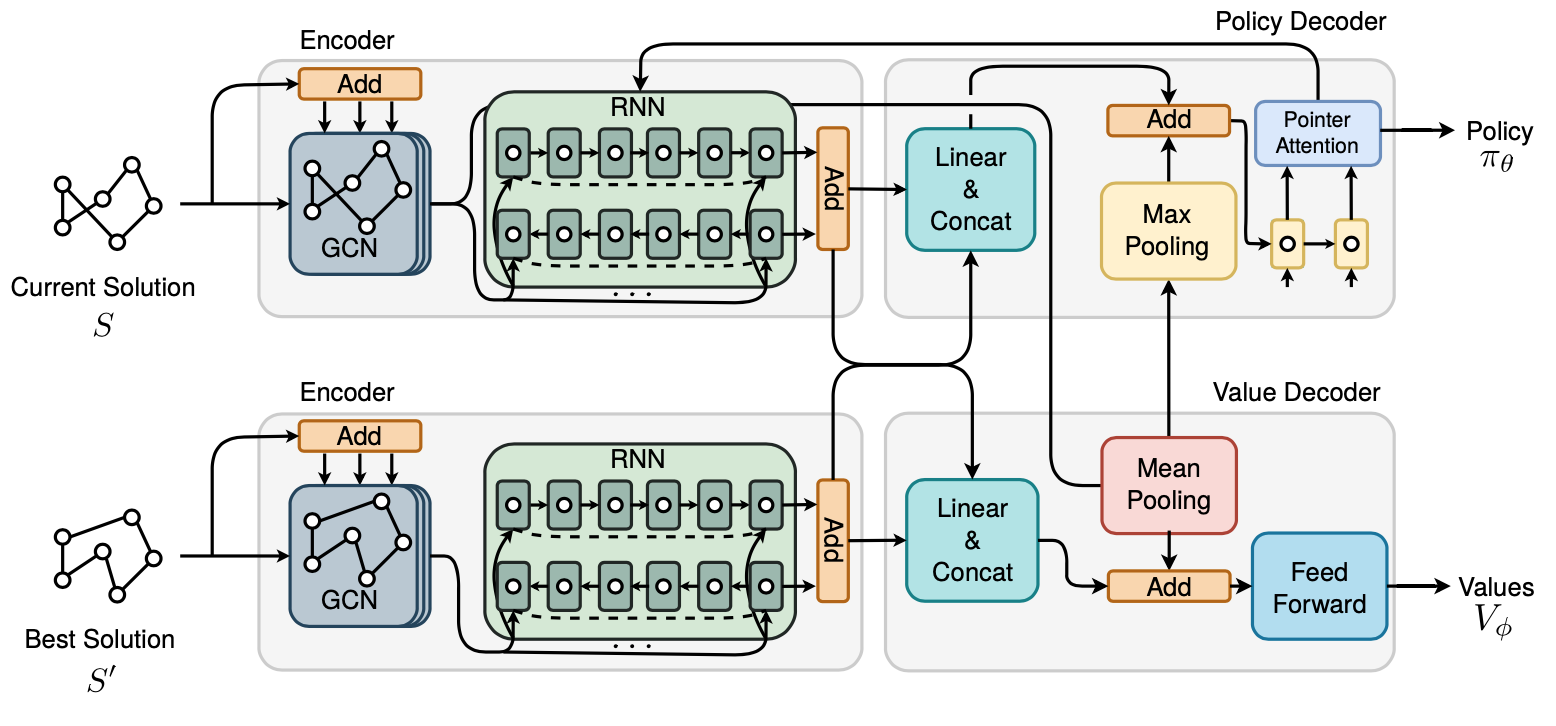
\includegraphics[width=4in]{Lec1-2OPT-NN.png}
	 \end{figure}
	 
	 \begin{itemize}
	 	\item We can run 2-OPT on any  edge-pair. 
		\item How to select an appropriate edge-pair? Using NN and RL [Roberto2020].
		
	 \end{itemize}


}

\frame{
	\frametitle{Extension: 3-OPT and LKH technique }
	
	 \begin{figure}
	 	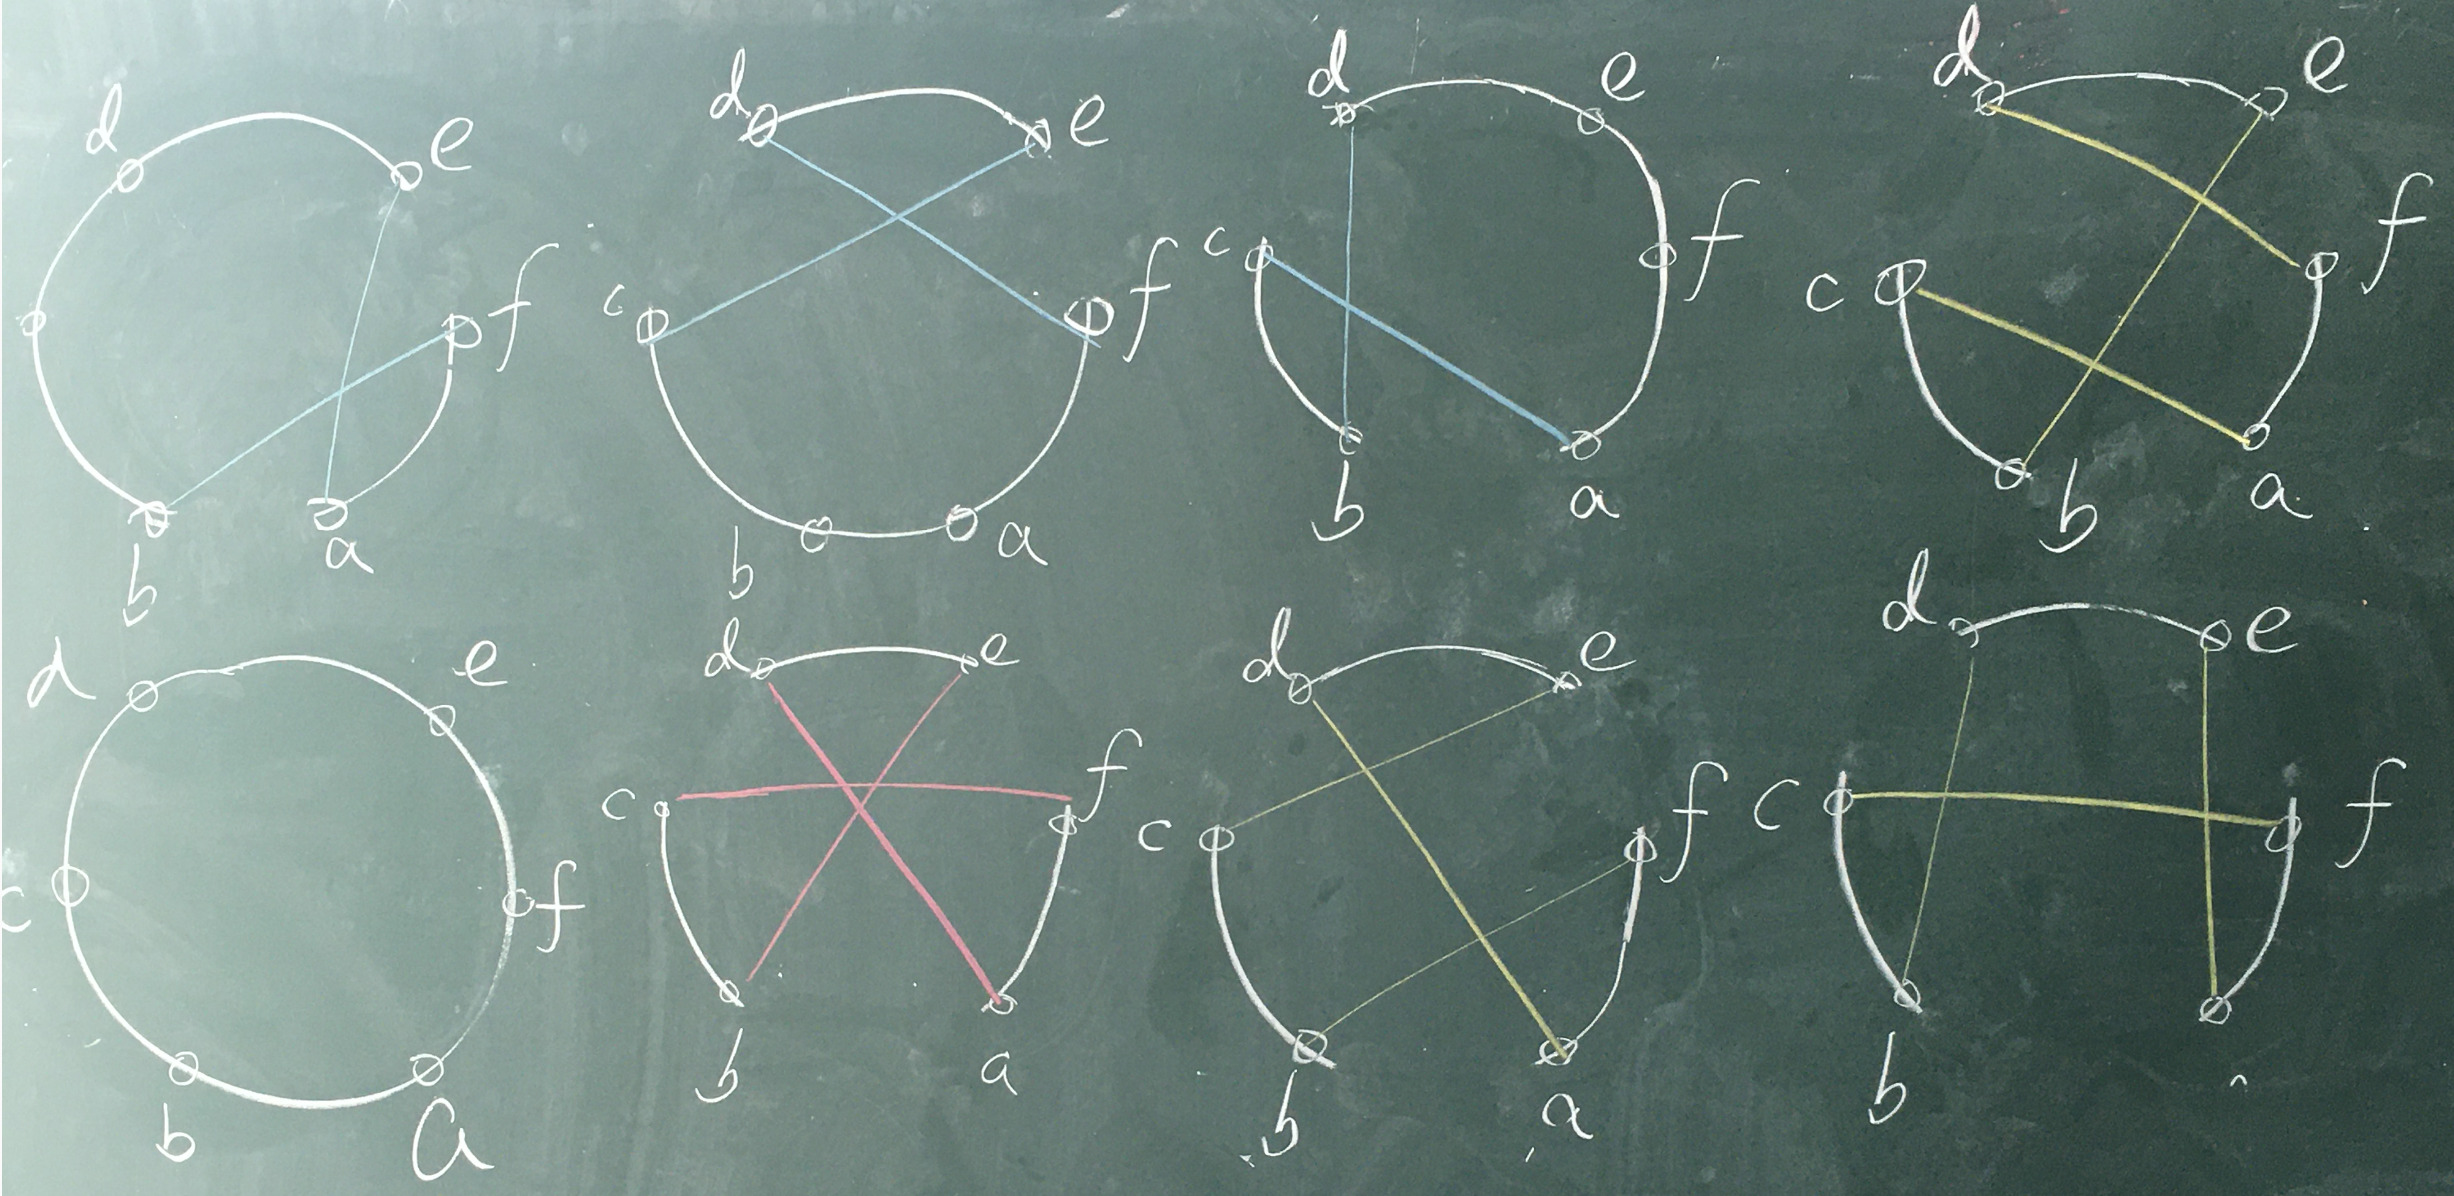
\includegraphics[width=4in]{L1-3OPT.jpg}
	 \end{figure}
	 
	 \begin{itemize}
	 	\item Selecting three edge $(a,b)$, $(c,d)$, and $(e,f)$, and applying $2-OPT$ and $3-OPT$ on them, we will have a total of 7 possible new tours. 
		\item The LK-1 technique uses up to sequential $5-OPT$ as well as  non-sequential $4-OPT$.  
	 \end{itemize}
}


\frame{
\begin{block}{}
{\bf Trial 3: ``Intelligent" enumeration strategy }
\end{block}
}


\frame{
	\frametitle{ Solution form }
	%{\sc Backtracking}: enumerate all possible complete solutions }

	\begin{itemize}
		\item Note that a complete solution can be expressed as a sequence of $n$ edges. Given a certain order of the $m$ edges, a complete solution can be represented as $X = [x_{1}, x_{2}, ..., x_{m}]$, where  $x_{i}=1$ if the edge $i$ was used in the tour, and $x_i = 0$ otherwise. 
		\item For example, the tour $a \rightarrow b\rightarrow c\rightarrow  d\rightarrow  e\rightarrow a $ can be represented as $X=[1, 0, 0, 1, 1, 0, 0, 1, 0, 1]$. 
		\item As every solution is a combination of $m$ items, we can enumerate all possible solutions. 
	\end{itemize} 

\begin{figure}
	\begin{tikzpicture}[scale=0.9, auto,swap]

    \foreach \pos/ \name in {{(-2,0)/a},{(2,0)/b}, {(-1,1.6)/e}, {(1,1.6)/c}, {(0,3.2)/d}} 
        \node[smallvertex,fill=blue!20] (\name) at \pos{$\name$};
     
    % Connect vertices with edges and draw weights
     %   \foreach \source/ \dest/\weight in {a/b/{3},   c/a/{4}, e/a/{7}, a/d/{2}, b/c/{4}, b/d/{6}, e/b/{3}, c/d/{5}, c/e/{8}, d/e/{6}}
    \foreach \source/ \dest/\weight in {a/b/{e_{1}{:}\  3},   a/c/{}, e/a/{e_{5}{:}\  7}, b/c/{e_{4}{:}\  4}, b/e/{}, c/d/{e_{8}{:}\  5}, c/e/{e_{9}{:}\  8}, d/e/{e_{10}{:}\  6}}
        \path[undirectededge] (\source) -- node[weight] {\tiny $\weight$} (\dest);
         
    \draw[thick] (a)   to [out=140, in=180] node[left] {\tiny $e_{3}{:}\  2$} (d);   
        \draw[thick] (b)   to [out=40, in=0] node[right] {\tiny $e_{6}{:}\  6$} (d);   
        
       \foreach \source/ \dest/\weight in {a/b/,   b/c/,  c/d/, d/e/, e/a/}
        \path[undirectededge, blue] (\source) -- node[weight] {$\weight$} (\dest);

	\node[] at (-0.9, 0.3) {\tiny $e_{2}{:}\  4$}; 
	\node[] at (0.9, 0.3) {\tiny $e_{7}{:}\  3$}; 

	%	$e_1=<a, b>, e_2=<a, c>, e_3 = <a, d>, e_4=<b, c>, e_5=<b, d>, e_6 = <b, e>, e_7=<c, d>, e_8=<c, e>, e_9=<d,e>$.  
        
%           \node at (4,3) {\small $e_{1}{:}\  <a, b>$}; 
%           \node at (4,2.6) {\small $e_{2}{:}\  <a, c>$};        
%           \node at (4,2.2) {\small $e_{3}{:}\  <a, d>$};        
%           \node at (4,1.8) {\small $e_{4}{:}\  <b, c>$};        
%           \node at (4,1.4) {\small $e_{5}{:}\  <b, d>$};        
%           \node at (4,1.0) {\small $e_{6}{:}\  <b, e>$};        
%           \node at (4,0.6) {\small $e_{7}{:}\  <c, d>$};        
%           \node at (4,0.2) {\small $e_{8}{:}\  <c, e>$};        
%            \node at (4,-0.2) {\small $e_{9}{:}\  <d, e>$};        
            
\end{tikzpicture}
\end{figure}

} 

\frame{
	\frametitle{Organizing solutions into a partial solution tree}
\begin{figure}
\begin{tikzpicture}[scale=.9, auto,swap]

	\def\x{3.4}; 
	\def\y{\x / 2}; 
	\def\z{\y / 2};
	\def\r{\z / 1.5};
	\def\d{0.1};
	\def\h{1};
	
%layer 1	
    \foreach \pos/\name/\label in {{(0,0)/root/}, {(-\x,-1*\h)/L/}, {(\x,-1*\h)/R/}}  
        \node[tinyvertex,draw=black, fill=white!20] (\name) at \pos {};
%layer 2	
    \def\base{-\x};
    \foreach \pos/\name/\label in {{( \base - \y, -2*\h)/LL/}, {( \base + \y,-2*\h)/LR/}}  
        \node[tinyvertex,draw=black, fill=white!20] (\name) at \pos {};	
    
    \def\base{\x};
    \foreach \pos/\name/\label in {{( \base - \y, -2*\h)/RL/}, {( \base + \y,-2*\h)/RR/}}  
        \node[tinyvertex,draw=black, fill=white!20] (\name) at \pos {};
%layer 3	
%    \def\base{-\x - \y};
%    \foreach \pos/\name/\label in {{( \base - \z, -3*\h)/LLL/}, {( \base + \z,-3*\h)/LLR/}}  
%        \node[tinyvertex,draw=black, fill=white!20] (\name) at \pos {};	      
    \def\base{-\x + \y};
    \foreach \pos/\name/\label in {{( \base - \z, -3*\h)/LRL/}, {( \base + \z,-3*\h)/LRR/}}  
        \node[tinyvertex,draw=black, fill=white!20] (\name) at \pos {};	
    
    \def\base{\x - \y};
    \foreach \pos/\name/\label in {{( \base - \z, -3*\h)/RLL/}, {( \base + \z,-3*\h)/RLR/}}  
        \node[tinyvertex,draw=black, fill=white!20] (\name) at \pos {};	      
        
    \def\base{-\x - \y};
    \foreach \pos/\name/\label in {{( \base + \z, -3*\h)/LLR/}}  
        \node[tinyvertex,draw=black, fill=white!20] (\name) at \pos {};	    

    \def\base{\x + \y};
    \foreach \pos/\name/\label in {{( \base - \z, -3*\h)/RRL/}}  
        \node[tinyvertex,draw=black, fill=white!20] (\name) at \pos {};	    

%    \def\base{\x + \y};
%    \foreach \pos/\name/\label in {{( \base - \z, -3*\h)/RRL/}, {( \base + \z,-3*\h)/RRR/}}  
%        \node[tinyvertex,draw=black, fill=white!20] (\name) at \pos {};	
   
 %layer 4 
%        \def\base{-\x + \y - \z};
%    \foreach \pos/\name/\label in {{( \base - \r, -4*\h)/LRLL/}, {( \base + \r,-4*\h)/LRLR/}}  
%        \node[tinyvertex,draw=black, fill=blue!20] (\name) at \pos {};	  
    \def\base{-\x - \y + \z};
    \foreach \pos/\name/\label in {{( \base + \r, -4*\h)/LLRR/}}  
        \node[tinyvertex,draw=black, fill=white!20] (\name) at \pos {};	  

    \def\base{-\x + \y + \z};
    \foreach \pos/\name/\label in {{( \base + \r, -4*\h)/LRRR/}}  
        \node[tinyvertex,draw=black, fill=white!20] (\name) at \pos {};	  
    \foreach \pos/\name/\label in {{( \base - \r, -4*\h)/LRRL/}}  
        \node[tinyvertex,draw=black, fill=white!20] (\name) at \pos {};	  

%        \node[] at (-\x -\y, -3*\h ) {$\dots$}; 
%        \node[] at (-\x -\y + \z, -4*\h ) {$\dots$}; 

%        \node[] at (-\x +\y - \z, -4*\h ) {$\dots$}; 
%        \node[] at (-\x +\y + \z, -4*\h ) {$\dots$}; 
%        \node[] at (\x -\y + \z, -4*\h ) {$\dots$}; 
                 
    \def\base{\x - \y + \z};
    \foreach \pos/\name/\label in {{( \base - \r, -4*\h)/RLRL/}, {( \base + \r, -4*\h)/RLRR/}}  
        \node[tinyvertex,draw=black, fill=white!20] (\name) at \pos {};	     

    \def\base{\x + \y - \z};
    \foreach \pos/\name/\label in {{( \base - \r, -4*\h)/RRLL/}, {( \base + \r, -4*\h)/RRLR/}}  
        \node[tinyvertex,draw=black, fill=white!20] (\name) at \pos {};	     

   %   \node[] at (\x - \y + \z, -4*\h ) {$\dots$}; 
 %     \node[] at (\x - \y - \z, -4*\h ) {$\dots$}; 

%      \node[] at (\x + \y, -3*\h ) {$\dots$}; 
%      \node[] at (\x + \y - \z, -4*\h ) {$\dots$}; 
   
   
           \def\base{\x - \y - \z};
           \def\r{\z/1.5};
    \foreach \pos/\name/\label in {{( \base - \r, -4*\h)/RLLL/}, {( \base + \r,-4*\h)/RLLR/}}  
        \node[tinyvertex,draw=black,fill=red] (\name) at \pos {};	  

           \def\base{-\x + \y - \z};
           \def\r{\z/1.5};
    \foreach \pos/\name/\label in {{( \base - \r, -4*\h)/LRLL/}, {( \base + \r,-4*\h)/LRLR/}}  
        \node[tinyvertex,draw=black,fill=red] (\name) at \pos {};	  

%%Layer 5 
%           \def\base{\x - \y + \z + \r};
%           \def\s{\z/1.5};
%    \foreach \pos/\name/\label in {{( \base - \s, -5*\h)/RLRRL/}, {( \base + \s,-5*\h)/RLRRR/}}  
%        \node[tinyvertex,draw=black,fill=white!20] (\name) at \pos {};	  
%
%%Layer 6 
%           \def\base{\x - \y + \z + \r + \s};
%           \def\t{\z/1.5};
%    \foreach \pos/\name/\label in {{( \base - \t, -6*\h)/RLRRRL/}, {( \base + \t,-6*\h)/RLRRRR/}}  
%        \node[tinyvertex,draw=black,fill=white!20] (\name) at \pos {};	  
%    \foreach \pos/\name/\label in {{( \base + \t,-6*\h)/RLRRRR/}}  
%        \node[tinyvertex,draw=black,fill=blue!20] (\name) at \pos {};	  

             
    % Connect vertices with edges and draw weights
  	\foreach \source/ \dest /\weight in {root/L/{x_1=1}, R/root/{0}}         
		\path[undirectededge] (\source) -- node[weight] {\tiny{$\weight$} } (\dest);
	%layer 2
	 \foreach \source/ \dest /\weight in {L/LL/{x_2=1}, LR/L/{0}}         
		\path[undirectededge] (\source) -- node[weight] {\tiny{$\weight$} } (\dest);

	 \foreach \source/ \dest /\weight in {R/RL/{1}, RR/R/{0}}         
		\path[undirectededge] (\source) -- node[weight] {\tiny{$\weight$} } (\dest);

	%layer 3
	 \foreach \source/ \dest /\weight in { LL/LLR/{x_3=0}}         
		\path[undirectededge] (\source) -- node[weight] {\tiny{$\weight$} } (\dest);

	 \foreach \source/ \dest /\weight in {LR/LRL/{1}, LRR/LR/{0}}         
		\path[undirectededge] (\source) -- node[weight] {\tiny{$\weight$} } (\dest);
	
	\foreach \source/ \dest /\weight in {RL/RLL/{1}, RLR/RL/{0}}         
		\path[undirectededge] (\source) -- node[weight] {\tiny{$\weight$} } (\dest);

	\foreach \source/ \dest /\weight in {RR/RRL/{1}}         
		\path[undirectededge] (\source) -- node[weight] {\tiny{$\weight$} } (\dest);

%	 \foreach \source/ \dest /\weight in {RR/RRL/{0}, RRR/RR/{1}}         
%		\path[undirectededge] (\source) -- node[weight] {\tiny{$\weight$} } (\dest);
	
	%layer 4 
         \foreach \source/ \dest /\weight in {RLL/RLLL/{1}, RLLR/RLL/{0}}         
		\path[undirectededge] (\source) -- node[weight] {\tiny{$\weight$} } (\dest);
	\foreach \source/ \dest /\weight in {LRL/LRLL/{1}, LRLR/LRL/{0}}         
		\path[undirectededge] (\source) -- node[weight] {\tiny{$\weight$} } (\dest);

         \foreach \source/ \dest /\weight in {LLR/LLRR/{\dots\qquad x_4=0}}         
		\path[undirectededge] (\source) -- node[weight] {\tiny{$\weight$} } (\dest);

         \foreach \source/ \dest /\weight in {LRR/LRRL/{1}, LRRR/LRR/{0}}         
		\path[undirectededge] (\source) -- node[weight] {\tiny{$\weight$} } (\dest);

         \foreach \source/ \dest /\weight in {RLR/RLRL/{1}, RLRR/RLR/{0}}         
		\path[undirectededge] (\source) -- node[weight] {\tiny{$\weight$} } (\dest);

         \foreach \source/ \dest /\weight in {RRL/RRLL/{1}, RRLR/RRL/{0\qquad \dots}}         
		\path[undirectededge] (\source) -- node[weight] {\tiny{$\weight$} } (\dest);

%	%layer 5
%         \foreach \source/ \dest /\weight in {RLRR/RLRRL/{x_5=0}, RLRRR/RLRR/{1}}         
%		\path[undirectededge] (\source) -- node[weight] {\tiny{$\weight$} } (\dest);
%%         \foreach \source/ \dest /\weight in {RRR/RRRL/{0}, RRR/RRRR/{1}}         
%%		\path[undirectededge] (\source) -- node[weight] {\tiny{$\weight$} } (\dest);
%
%	%layer 6
%         \foreach \source/ \dest /\weight in {RLRRR/RLRRRL/{x_6=0}, RLRRRR/RLRRR/{1}}         
%		\path[undirectededge] (\source) -- node[weight] {\tiny{$\weight$} } (\dest);
%         \foreach \source/ \dest /\weight in {RRR/RRRL/{0}, RRR/RRRR/{1}}         
%		\path[undirectededge] (\source) -- node[weight] {\tiny{$\weight$} } (\dest);

	
%label 			
    \foreach \pos/\name/\label in {{(0+\d,0)/root/X=??????????},  {(-\x+\d,-1*\h)/L/1?????????}, {(\x+\d,-1*\h)/R/0?????????}} 
        \node[right] at \pos {\tiny{ $\label$}};
%layer 2	
    \def\base{-\x};
    \foreach \pos/\name/\label in {{( \base + \y +\d,-2*\h)/LR/10????????}}  
        \node[right] at \pos {\tiny{ $\label$}};
    \foreach \pos/\name/\label in {{( \base - \y + \d, -2*\h)/LL/11????????}}  
        \node[right] at \pos {\tiny{ $\label$}};
            
    \def\base{\x};
    \foreach \pos/\name/\label in {{( \base - \y+\d, -2*\h)/RL/01????????}}  
        \node[right] at \pos {\tiny{ $\label$}};
    \foreach \pos/\name/\label in {{( \base + \y+\d,-2*\h)/RR/00????????}}  
        \node[right] at \pos {\tiny{ $\label$}};


%layer 3
    \def\base{-\x - \y};
    \foreach \pos/\name/\label in {{( \base - \z, -3*\h)/LLL/}, {( \base + \z,-3*\h)/LLR/}}  
        \node[right] at \pos {\tiny{$\label$}};	 
             
    \def\base{-\x + \y};
    \foreach \pos/\name/\label in {{( \base - \z, -3*\h)/LRL/101?0?????}, {( \base + \z,-3*\h)/LRR/}}  
        \node[right] at \pos {\tiny{$\label$}};	 
    
    \def\base{\x - \y};
    \foreach \pos/\name/\label in {{( \base - \z, -3*\h)/RLL/}, {( \base + \z,-3*\h)/RLR/}}  
        \node[right] at \pos {\tiny{$\label$}};	 

    \def\base{\x + \y};
    \foreach \pos/\name/\label in {{( \base - \z, -3*\h)/RRL/}, {( \base + \z,-3*\h)/RRR/}}  
        \node[right] at \pos {\tiny{$\label$}};	 
   
  
   
% %layer 4
%         \def\base{-\x + \y - \z};
%    \foreach \pos/\name/\label in {{( \base - \r, -4*\h)/LRLL/[0,1,0,0]}, {( \base + \r,-4*\h)/LRLR/[0,1,0,1]}}  
%        \node[below] at \pos {\tiny{$\label$}};	      
%         
%         \def\base{\x - \y - \z};
%    \foreach \pos/\name/\label in {{( \base - \r, -4*\h)/RLLL/[1,0,0,0]}, {( \base + \r,-4*\h)/RLLR/[1,0,0,1]}}  
%        \node[below] at \pos {\tiny{$\label$}};	      
     
      %layer 3
  %RLR 
%  \def\d{0.3};
%  \node[] at (\x - \y + \z + 0.2, -3*\h + \d ) {\tiny $010?1?????$}; 
  %RLL
 % \node[] at (\x - \y - \z + 0.5, -3*\h ) {\tiny $011?0?????$}; 
    
  %LRR 
%  \def\d{0.3};
%  \node[] at (-\x + \y + \z, -3*\h - \d ) {\tiny $100?1?????$}; 
  %LRL
 % \node[] at (\x - \y - \z + 0.5, -3*\h ) {\tiny $101?0?????$}; 
    
  %layer 4
 %RLLL
  \def\d{0.3};
  \node[red] at (\x - \y - \z - \r - 0.3, -4*\h - \d ) {\tiny $0111001001$}; 
 %RLLR
  \def\d{0.3};
  \node[red] at (\x - \y - \z + \r + 0.3, -4*\h - \d ) {\tiny $0110011010$}; 
 
  %RRLR
  \def\d{0.3};
  \node[] at (\x  + \y - \z + \r , -4*\h - \d ) {\tiny \dots }; 

  
%LRLL
  \def\d{0.3};
  \node[red] at (-\x + \y - \z - \r - 0.3, -4*\h - \d ) {\tiny $1011000011$}; 
 %LRLR
  \def\d{0.3};
  \node[red] at (-\x + \y - \z + \r + 0.3, -4*\h - \d ) {\tiny $1010001110$}; 

  %RRLR
  \def\d{0.3};
  \node[] at (\x + \y - \z - \r , -4*\h - \d ) {\tiny \dots}; 

 
   \end{tikzpicture}
\end{figure}


\begin{itemize}
		\begin{footnotesize}

  \item Partial solution tree: 

	\begin{itemize}
		\begin{footnotesize}
		\item Leaf node: representing \textcolor{red}{\bf a complete solution} associated with an objective function value, e.g., $X=1011000011$ has an objective function value of 23. 
   		\item Internal node: representing \textcolor{red}{\bf a partial solution}, where only a subset of items (in the path from root to the node) are known, e.g., $X=10????????$ refers to tours including  $e_{1} $ but excluding $e_{2}$. 
		%Thus, it also represents \textcolor{red}{\bf a sub-problem} to determine the remainder items, or  \textcolor{red}{\bf a set of complete solutions} of the subtree rooted at this partial solution,  e.g., $X=101?0?????$ represents two nodes in red. 
%			\begin{itemize}
%				\item A partial solution represents a sub-problem. 
%				\item A partial solution represents a set of complete solutions w.r.t. the sub-problem.
%			\end{itemize}
	\end{footnotesize}
	\end{itemize}
	\end{footnotesize}
\end{itemize}
}

\frame{
	\frametitle{Two alternative views of a partial solution} 
\begin{figure}
\begin{tikzpicture}[scale=.9, auto,swap]

	\def\x{3.4}; 
	\def\y{\x / 2}; 
	\def\z{\y / 2};
	\def\r{\z / 1.5};
	\def\d{0.1};
	\def\h{1};
	
%layer 1	
    \foreach \pos/\name/\label in {{(0,0)/root/}, {(-\x,-1*\h)/L/}, {(\x,-1*\h)/R/}}  
        \node[tinyvertex,draw=black, fill=white!20] (\name) at \pos {};
%layer 2	
    \def\base{-\x};
    \foreach \pos/\name/\label in {{( \base - \y, -2*\h)/LL/}, {( \base + \y,-2*\h)/LR/}}  
        \node[tinyvertex,draw=black, fill=white!20] (\name) at \pos {};	
    
    \def\base{\x};
    \foreach \pos/\name/\label in {{( \base - \y, -2*\h)/RL/}, {( \base + \y,-2*\h)/RR/}}  
        \node[tinyvertex,draw=black, fill=white!20] (\name) at \pos {};
%layer 3	
%    \def\base{-\x - \y};
%    \foreach \pos/\name/\label in {{( \base - \z, -3*\h)/LLL/}, {( \base + \z,-3*\h)/LLR/}}  
%        \node[tinyvertex,draw=black, fill=white!20] (\name) at \pos {};	      
    \def\base{-\x + \y};
    \foreach \pos/\name/\label in {{( \base - \z, -3*\h)/LRL/}, {( \base + \z,-3*\h)/LRR/}}  
        \node[tinyvertex,draw=black, fill=white!20] (\name) at \pos {};	
    
    \def\base{\x - \y};
    \foreach \pos/\name/\label in {{( \base - \z, -3*\h)/RLL/}, {( \base + \z,-3*\h)/RLR/}}  
        \node[tinyvertex,draw=black, fill=white!20] (\name) at \pos {};	      
        
    \def\base{-\x - \y};
    \foreach \pos/\name/\label in {{( \base + \z, -3*\h)/LLR/}}  
        \node[tinyvertex,draw=black, fill=white!20] (\name) at \pos {};	    

    \def\base{\x + \y};
    \foreach \pos/\name/\label in {{( \base - \z, -3*\h)/RRL/}}  
        \node[tinyvertex,draw=black, fill=white!20] (\name) at \pos {};	    

%    \def\base{\x + \y};
%    \foreach \pos/\name/\label in {{( \base - \z, -3*\h)/RRL/}, {( \base + \z,-3*\h)/RRR/}}  
%        \node[tinyvertex,draw=black, fill=white!20] (\name) at \pos {};	
   
 %layer 4 
%        \def\base{-\x + \y - \z};
%    \foreach \pos/\name/\label in {{( \base - \r, -4*\h)/LRLL/}, {( \base + \r,-4*\h)/LRLR/}}  
%        \node[tinyvertex,draw=black, fill=blue!20] (\name) at \pos {};	  
    \def\base{-\x - \y + \z};
    \foreach \pos/\name/\label in {{( \base + \r, -4*\h)/LLRR/}}  
        \node[tinyvertex,draw=black, fill=white!20] (\name) at \pos {};	  

    \def\base{-\x + \y + \z};
    \foreach \pos/\name/\label in {{( \base + \r, -4*\h)/LRRR/}}  
        \node[tinyvertex,draw=black, fill=white!20] (\name) at \pos {};	  
    \foreach \pos/\name/\label in {{( \base - \r, -4*\h)/LRRL/}}  
        \node[tinyvertex,draw=black, fill=white!20] (\name) at \pos {};	  

%        \node[] at (-\x -\y, -3*\h ) {$\dots$}; 
%        \node[] at (-\x -\y + \z, -4*\h ) {$\dots$}; 

%        \node[] at (-\x +\y - \z, -4*\h ) {$\dots$}; 
%        \node[] at (-\x +\y + \z, -4*\h ) {$\dots$}; 
%        \node[] at (\x -\y + \z, -4*\h ) {$\dots$}; 
                 
    \def\base{\x - \y + \z};
    \foreach \pos/\name/\label in {{( \base - \r, -4*\h)/RLRL/}, {( \base + \r, -4*\h)/RLRR/}}  
        \node[tinyvertex,draw=black, fill=white!20] (\name) at \pos {};	     

    \def\base{\x + \y - \z};
    \foreach \pos/\name/\label in {{( \base - \r, -4*\h)/RRLL/}, {( \base + \r, -4*\h)/RRLR/}}  
        \node[tinyvertex,draw=black, fill=white!20] (\name) at \pos {};	     

   %   \node[] at (\x - \y + \z, -4*\h ) {$\dots$}; 
 %     \node[] at (\x - \y - \z, -4*\h ) {$\dots$}; 

%      \node[] at (\x + \y, -3*\h ) {$\dots$}; 
%      \node[] at (\x + \y - \z, -4*\h ) {$\dots$}; 
   
   
           \def\base{\x - \y - \z};
           \def\r{\z/1.5};
    \foreach \pos/\name/\label in {{( \base - \r, -4*\h)/RLLL/}, {( \base + \r,-4*\h)/RLLR/}}  
        \node[tinyvertex,draw=black,fill=red] (\name) at \pos {};	  

           \def\base{-\x + \y - \z};
           \def\r{\z/1.5};
    \foreach \pos/\name/\label in {{( \base - \r, -4*\h)/LRLL/}, {( \base + \r,-4*\h)/LRLR/}}  
        \node[tinyvertex,draw=black,fill=red] (\name) at \pos {};	  

%%Layer 5 
%           \def\base{\x - \y + \z + \r};
%           \def\s{\z/1.5};
%    \foreach \pos/\name/\label in {{( \base - \s, -5*\h)/RLRRL/}, {( \base + \s,-5*\h)/RLRRR/}}  
%        \node[tinyvertex,draw=black,fill=white!20] (\name) at \pos {};	  
%
%%Layer 6 
%           \def\base{\x - \y + \z + \r + \s};
%           \def\t{\z/1.5};
%    \foreach \pos/\name/\label in {{( \base - \t, -6*\h)/RLRRRL/}, {( \base + \t,-6*\h)/RLRRRR/}}  
%        \node[tinyvertex,draw=black,fill=white!20] (\name) at \pos {};	  
%    \foreach \pos/\name/\label in {{( \base + \t,-6*\h)/RLRRRR/}}  
%        \node[tinyvertex,draw=black,fill=blue!20] (\name) at \pos {};	  

             
    % Connect vertices with edges and draw weights
  	\foreach \source/ \dest /\weight in {root/L/{x_1=1}, R/root/{0}}         
		\path[undirectededge] (\source) -- node[weight] {\tiny{$\weight$} } (\dest);
	%layer 2
	 \foreach \source/ \dest /\weight in {L/LL/{x_2=1}, LR/L/{0}}         
		\path[undirectededge] (\source) -- node[weight] {\tiny{$\weight$} } (\dest);

	 \foreach \source/ \dest /\weight in {R/RL/{1}, RR/R/{0}}         
		\path[undirectededge] (\source) -- node[weight] {\tiny{$\weight$} } (\dest);

	%layer 3
	 \foreach \source/ \dest /\weight in { LL/LLR/{x_3=0}}         
		\path[undirectededge] (\source) -- node[weight] {\tiny{$\weight$} } (\dest);

	 \foreach \source/ \dest /\weight in {LR/LRL/{1}, LRR/LR/{0}}         
		\path[undirectededge] (\source) -- node[weight] {\tiny{$\weight$} } (\dest);
	
	\foreach \source/ \dest /\weight in {RL/RLL/{1}, RLR/RL/{0}}         
		\path[undirectededge] (\source) -- node[weight] {\tiny{$\weight$} } (\dest);

	\foreach \source/ \dest /\weight in {RR/RRL/{1}}         
		\path[undirectededge] (\source) -- node[weight] {\tiny{$\weight$} } (\dest);

%	 \foreach \source/ \dest /\weight in {RR/RRL/{0}, RRR/RR/{1}}         
%		\path[undirectededge] (\source) -- node[weight] {\tiny{$\weight$} } (\dest);
	
	%layer 4 
         \foreach \source/ \dest /\weight in {RLL/RLLL/{1}, RLLR/RLL/{0}}         
		\path[undirectededge] (\source) -- node[weight] {\tiny{$\weight$} } (\dest);
	\foreach \source/ \dest /\weight in {LRL/LRLL/{1}, LRLR/LRL/{0}}         
		\path[undirectededge] (\source) -- node[weight] {\tiny{$\weight$} } (\dest);

         \foreach \source/ \dest /\weight in {LLR/LLRR/{\dots\qquad x_4=0}}         
		\path[undirectededge] (\source) -- node[weight] {\tiny{$\weight$} } (\dest);

         \foreach \source/ \dest /\weight in {LRR/LRRL/{1}, LRRR/LRR/{0}}         
		\path[undirectededge] (\source) -- node[weight] {\tiny{$\weight$} } (\dest);

         \foreach \source/ \dest /\weight in {RLR/RLRL/{1}, RLRR/RLR/{0}}         
		\path[undirectededge] (\source) -- node[weight] {\tiny{$\weight$} } (\dest);

         \foreach \source/ \dest /\weight in {RRL/RRLL/{1}, RRLR/RRL/{0\qquad \dots}}         
		\path[undirectededge] (\source) -- node[weight] {\tiny{$\weight$} } (\dest);

%	%layer 5
%         \foreach \source/ \dest /\weight in {RLRR/RLRRL/{x_5=0}, RLRRR/RLRR/{1}}         
%		\path[undirectededge] (\source) -- node[weight] {\tiny{$\weight$} } (\dest);
%%         \foreach \source/ \dest /\weight in {RRR/RRRL/{0}, RRR/RRRR/{1}}         
%%		\path[undirectededge] (\source) -- node[weight] {\tiny{$\weight$} } (\dest);
%
%	%layer 6
%         \foreach \source/ \dest /\weight in {RLRRR/RLRRRL/{x_6=0}, RLRRRR/RLRRR/{1}}         
%		\path[undirectededge] (\source) -- node[weight] {\tiny{$\weight$} } (\dest);
%         \foreach \source/ \dest /\weight in {RRR/RRRL/{0}, RRR/RRRR/{1}}         
%		\path[undirectededge] (\source) -- node[weight] {\tiny{$\weight$} } (\dest);

	
%label 			
    \foreach \pos/\name/\label in {{(0+\d,0)/root/X=??????????},  {(-\x+\d,-1*\h)/L/1?????????}, {(\x+\d,-1*\h)/R/0?????????}} 
        \node[right] at \pos {\tiny{ $\label$}};
%layer 2	
    \def\base{-\x};
    \foreach \pos/\name/\label in {{( \base + \y +\d,-2*\h)/LR/10????????}}  
        \node[right] at \pos {\tiny{ $\label$}};
    \foreach \pos/\name/\label in {{( \base - \y + \d, -2*\h)/LL/11????????}}  
        \node[right] at \pos {\tiny{ $\label$}};
            
    \def\base{\x};
    \foreach \pos/\name/\label in {{( \base - \y+\d, -2*\h)/RL/01????????}}  
        \node[right] at \pos {\tiny{ $\label$}};
    \foreach \pos/\name/\label in {{( \base + \y+\d,-2*\h)/RR/00????????}}  
        \node[right] at \pos {\tiny{ $\label$}};


%layer 3
    \def\base{-\x - \y};
    \foreach \pos/\name/\label in {{( \base - \z, -3*\h)/LLL/}, {( \base + \z,-3*\h)/LLR/}}  
        \node[right] at \pos {\tiny{$\label$}};	 
             
    \def\base{-\x + \y};
    \foreach \pos/\name/\label in {{( \base - \z, -3*\h)/LRL/101?0?????}, {( \base + \z,-3*\h)/LRR/}}  
        \node[right] at \pos {\tiny{$\label$}};	 
    
    \def\base{\x - \y};
    \foreach \pos/\name/\label in {{( \base - \z, -3*\h)/RLL/}, {( \base + \z,-3*\h)/RLR/}}  
        \node[right] at \pos {\tiny{$\label$}};	 

    \def\base{\x + \y};
    \foreach \pos/\name/\label in {{( \base - \z, -3*\h)/RRL/}, {( \base + \z,-3*\h)/RRR/}}  
        \node[right] at \pos {\tiny{$\label$}};	 
   
  
   
% %layer 4
%         \def\base{-\x + \y - \z};
%    \foreach \pos/\name/\label in {{( \base - \r, -4*\h)/LRLL/[0,1,0,0]}, {( \base + \r,-4*\h)/LRLR/[0,1,0,1]}}  
%        \node[below] at \pos {\tiny{$\label$}};	      
%         
%         \def\base{\x - \y - \z};
%    \foreach \pos/\name/\label in {{( \base - \r, -4*\h)/RLLL/[1,0,0,0]}, {( \base + \r,-4*\h)/RLLR/[1,0,0,1]}}  
%        \node[below] at \pos {\tiny{$\label$}};	      
     
      %layer 3
  %RLR 
%  \def\d{0.3};
%  \node[] at (\x - \y + \z + 0.2, -3*\h + \d ) {\tiny $010?1?????$}; 
  %RLL
 % \node[] at (\x - \y - \z + 0.5, -3*\h ) {\tiny $011?0?????$}; 
    
  %LRR 
%  \def\d{0.3};
%  \node[] at (-\x + \y + \z, -3*\h - \d ) {\tiny $100?1?????$}; 
  %LRL
 % \node[] at (\x - \y - \z + 0.5, -3*\h ) {\tiny $101?0?????$}; 
    
  %layer 4
 %RLLL
  \def\d{0.3};
  \node[red] at (\x - \y - \z - \r - 0.3, -4*\h - \d ) {\tiny $0111001001$}; 
 %RLLR
  \def\d{0.3};
  \node[red] at (\x - \y - \z + \r + 0.3, -4*\h - \d ) {\tiny $0110011010$}; 
 
  %RRLR
  \def\d{0.3};
  \node[] at (\x  + \y - \z + \r , -4*\h - \d ) {\tiny \dots }; 

  
%LRLL
  \def\d{0.3};
  \node[red] at (-\x + \y - \z - \r - 0.3, -4*\h - \d ) {\tiny $1011000011$}; 
 %LRLR
  \def\d{0.3};
  \node[red] at (-\x + \y - \z + \r + 0.3, -4*\h - \d ) {\tiny $1010001110$}; 

  %RRLR
  \def\d{0.3};
  \node[] at (\x + \y - \z - \r , -4*\h - \d ) {\tiny \dots}; 

 
   \end{tikzpicture}
\end{figure}

\begin{itemize}

 		\begin{footnotesize}
%		\item Only a subset of items has been determined, i.e., $x_1=1$, $x_2 = 0$, $x_3 = 1$, $x_5=0$, corresponding to the path from root to the node. 
		%Leaf node: representing a complete solution associated with an objective function value, e.g., $X=1010001110$. 
   		\item A subproblem: to determine the \textcolor{red}{\bf unknown items}, e.g., $X=10????????$ means to find the shortest tour including $e_{1}$  but excluding $e_{2}$. 
		\item A collection of complete solutions: the leaf nodes of the subtree rooted at this partial solution,  e.g., $X=101?0?????$ represents two nodes in red $1011000011$ and $1010001110$. 
%			\begin{itemize}
%				\item A partial solution represents a sub-problem. 
%				\item A partial solution represents a set of complete solutions w.r.t. the sub-problem.
%			\end{itemize}

	\end{footnotesize}
\end{itemize}
}


\frame{
	\frametitle{Deduction rules for simplification} 
\begin{figure}
\begin{tikzpicture}[scale=.9, auto,swap]

	\def\x{3.4}; 
	\def\y{\x / 2}; 
	\def\z{\y / 2};
	\def\r{\z / 1.5};
	\def\d{0.1};
	\def\h{1};
	
%layer 1	
    \foreach \pos/\name/\label in {{(0,0)/root/}, {(-\x,-1*\h)/L/}, {(\x,-1*\h)/R/}}  
        \node[tinyvertex,draw=black, fill=white!20] (\name) at \pos {};
%layer 2	
    \def\base{-\x};
    \foreach \pos/\name/\label in {{( \base - \y, -2*\h)/LL/}, {( \base + \y,-2*\h)/LR/}}  
        \node[tinyvertex,draw=black, fill=white!20] (\name) at \pos {};	
    
    \def\base{\x};
    \foreach \pos/\name/\label in {{( \base - \y, -2*\h)/RL/}, {( \base + \y,-2*\h)/RR/}}  
        \node[tinyvertex,draw=black, fill=white!20] (\name) at \pos {};
%layer 3	
%    \def\base{-\x - \y};
%    \foreach \pos/\name/\label in {{( \base - \z, -3*\h)/LLL/}, {( \base + \z,-3*\h)/LLR/}}  
%        \node[tinyvertex,draw=black, fill=white!20] (\name) at \pos {};	      
    \def\base{-\x + \y};
    \foreach \pos/\name/\label in {{( \base - \z, -3*\h)/LRL/}, {( \base + \z,-3*\h)/LRR/}}  
        \node[tinyvertex,draw=black, fill=white!20] (\name) at \pos {};	
    
    \def\base{\x - \y};
    \foreach \pos/\name/\label in {{( \base - \z, -3*\h)/RLL/}, {( \base + \z,-3*\h)/RLR/}}  
        \node[tinyvertex,draw=black, fill=white!20] (\name) at \pos {};	      
        
    \def\base{-\x - \y};
    \foreach \pos/\name/\label in {{( \base + \z, -3*\h)/LLR/}}  
        \node[tinyvertex,draw=black, fill=white!20] (\name) at \pos {};	    

    \def\base{\x + \y};
    \foreach \pos/\name/\label in {{( \base - \z, -3*\h)/RRL/}}  
        \node[tinyvertex,draw=black, fill=white!20] (\name) at \pos {};	    

%    \def\base{\x + \y};
%    \foreach \pos/\name/\label in {{( \base - \z, -3*\h)/RRL/}, {( \base + \z,-3*\h)/RRR/}}  
%        \node[tinyvertex,draw=black, fill=white!20] (\name) at \pos {};	
   
 %layer 4 
%        \def\base{-\x + \y - \z};
%    \foreach \pos/\name/\label in {{( \base - \r, -4*\h)/LRLL/}, {( \base + \r,-4*\h)/LRLR/}}  
%        \node[tinyvertex,draw=black, fill=blue!20] (\name) at \pos {};	  
    \def\base{-\x - \y + \z};
    \foreach \pos/\name/\label in {{( \base + \r, -4*\h)/LLRR/}}  
        \node[tinyvertex,draw=black, fill=white!20] (\name) at \pos {};	  

    \def\base{-\x + \y + \z};
    \foreach \pos/\name/\label in {{( \base + \r, -4*\h)/LRRR/}}  
        \node[tinyvertex,draw=black, fill=white!20] (\name) at \pos {};	  
    \foreach \pos/\name/\label in {{( \base - \r, -4*\h)/LRRL/}}  
        \node[tinyvertex,draw=black, fill=white!20] (\name) at \pos {};	  

%        \node[] at (-\x -\y, -3*\h ) {$\dots$}; 
%        \node[] at (-\x -\y + \z, -4*\h ) {$\dots$}; 

%        \node[] at (-\x +\y - \z, -4*\h ) {$\dots$}; 
%        \node[] at (-\x +\y + \z, -4*\h ) {$\dots$}; 
%        \node[] at (\x -\y + \z, -4*\h ) {$\dots$}; 
                 
    \def\base{\x - \y + \z};
    \foreach \pos/\name/\label in {{( \base - \r, -4*\h)/RLRL/}, {( \base + \r, -4*\h)/RLRR/}}  
        \node[tinyvertex,draw=black, fill=white!20] (\name) at \pos {};	     

    \def\base{\x + \y - \z};
    \foreach \pos/\name/\label in {{( \base - \r, -4*\h)/RRLL/}, {( \base + \r, -4*\h)/RRLR/}}  
        \node[tinyvertex,draw=black, fill=white!20] (\name) at \pos {};	     

   %   \node[] at (\x - \y + \z, -4*\h ) {$\dots$}; 
 %     \node[] at (\x - \y - \z, -4*\h ) {$\dots$}; 

%      \node[] at (\x + \y, -3*\h ) {$\dots$}; 
%      \node[] at (\x + \y - \z, -4*\h ) {$\dots$}; 
   
   
           \def\base{\x - \y - \z};
           \def\r{\z/1.5};
    \foreach \pos/\name/\label in {{( \base - \r, -4*\h)/RLLL/}, {( \base + \r,-4*\h)/RLLR/}}  
        \node[tinyvertex,draw=black,fill=red] (\name) at \pos {};	  

           \def\base{-\x + \y - \z};
           \def\r{\z/1.5};
    \foreach \pos/\name/\label in {{( \base - \r, -4*\h)/LRLL/}, {( \base + \r,-4*\h)/LRLR/}}  
        \node[tinyvertex,draw=black,fill=red] (\name) at \pos {};	  

%%Layer 5 
%           \def\base{\x - \y + \z + \r};
%           \def\s{\z/1.5};
%    \foreach \pos/\name/\label in {{( \base - \s, -5*\h)/RLRRL/}, {( \base + \s,-5*\h)/RLRRR/}}  
%        \node[tinyvertex,draw=black,fill=white!20] (\name) at \pos {};	  
%
%%Layer 6 
%           \def\base{\x - \y + \z + \r + \s};
%           \def\t{\z/1.5};
%    \foreach \pos/\name/\label in {{( \base - \t, -6*\h)/RLRRRL/}, {( \base + \t,-6*\h)/RLRRRR/}}  
%        \node[tinyvertex,draw=black,fill=white!20] (\name) at \pos {};	  
%    \foreach \pos/\name/\label in {{( \base + \t,-6*\h)/RLRRRR/}}  
%        \node[tinyvertex,draw=black,fill=blue!20] (\name) at \pos {};	  

             
    % Connect vertices with edges and draw weights
  	\foreach \source/ \dest /\weight in {root/L/{x_1=1}, R/root/{0}}         
		\path[undirectededge] (\source) -- node[weight] {\tiny{$\weight$} } (\dest);
	%layer 2
	 \foreach \source/ \dest /\weight in {L/LL/{x_2=1}, LR/L/{0}}         
		\path[undirectededge] (\source) -- node[weight] {\tiny{$\weight$} } (\dest);

	 \foreach \source/ \dest /\weight in {R/RL/{1}, RR/R/{0}}         
		\path[undirectededge] (\source) -- node[weight] {\tiny{$\weight$} } (\dest);

	%layer 3
	 \foreach \source/ \dest /\weight in { LL/LLR/{x_3=0}}         
		\path[undirectededge] (\source) -- node[weight] {\tiny{$\weight$} } (\dest);

	 \foreach \source/ \dest /\weight in {LR/LRL/{1}, LRR/LR/{0}}         
		\path[undirectededge] (\source) -- node[weight] {\tiny{$\weight$} } (\dest);
	
	\foreach \source/ \dest /\weight in {RL/RLL/{1}, RLR/RL/{0}}         
		\path[undirectededge] (\source) -- node[weight] {\tiny{$\weight$} } (\dest);

	\foreach \source/ \dest /\weight in {RR/RRL/{1}}         
		\path[undirectededge] (\source) -- node[weight] {\tiny{$\weight$} } (\dest);

%	 \foreach \source/ \dest /\weight in {RR/RRL/{0}, RRR/RR/{1}}         
%		\path[undirectededge] (\source) -- node[weight] {\tiny{$\weight$} } (\dest);
	
	%layer 4 
         \foreach \source/ \dest /\weight in {RLL/RLLL/{1}, RLLR/RLL/{0}}         
		\path[undirectededge] (\source) -- node[weight] {\tiny{$\weight$} } (\dest);
	\foreach \source/ \dest /\weight in {LRL/LRLL/{1}, LRLR/LRL/{0}}         
		\path[undirectededge] (\source) -- node[weight] {\tiny{$\weight$} } (\dest);

         \foreach \source/ \dest /\weight in {LLR/LLRR/{\dots\qquad x_4=0}}         
		\path[undirectededge] (\source) -- node[weight] {\tiny{$\weight$} } (\dest);

         \foreach \source/ \dest /\weight in {LRR/LRRL/{1}, LRRR/LRR/{0}}         
		\path[undirectededge] (\source) -- node[weight] {\tiny{$\weight$} } (\dest);

         \foreach \source/ \dest /\weight in {RLR/RLRL/{1}, RLRR/RLR/{0}}         
		\path[undirectededge] (\source) -- node[weight] {\tiny{$\weight$} } (\dest);

         \foreach \source/ \dest /\weight in {RRL/RRLL/{1}, RRLR/RRL/{0\qquad \dots}}         
		\path[undirectededge] (\source) -- node[weight] {\tiny{$\weight$} } (\dest);

%	%layer 5
%         \foreach \source/ \dest /\weight in {RLRR/RLRRL/{x_5=0}, RLRRR/RLRR/{1}}         
%		\path[undirectededge] (\source) -- node[weight] {\tiny{$\weight$} } (\dest);
%%         \foreach \source/ \dest /\weight in {RRR/RRRL/{0}, RRR/RRRR/{1}}         
%%		\path[undirectededge] (\source) -- node[weight] {\tiny{$\weight$} } (\dest);
%
%	%layer 6
%         \foreach \source/ \dest /\weight in {RLRRR/RLRRRL/{x_6=0}, RLRRRR/RLRRR/{1}}         
%		\path[undirectededge] (\source) -- node[weight] {\tiny{$\weight$} } (\dest);
%         \foreach \source/ \dest /\weight in {RRR/RRRL/{0}, RRR/RRRR/{1}}         
%		\path[undirectededge] (\source) -- node[weight] {\tiny{$\weight$} } (\dest);

	
%label 			
    \foreach \pos/\name/\label in {{(0+\d,0)/root/X=??????????},  {(-\x+\d,-1*\h)/L/1?????????}, {(\x+\d,-1*\h)/R/0?????????}} 
        \node[right] at \pos {\tiny{ $\label$}};
%layer 2	
    \def\base{-\x};
    \foreach \pos/\name/\label in {{( \base + \y +\d,-2*\h)/LR/10????????}}  
        \node[right] at \pos {\tiny{ $\label$}};
    \foreach \pos/\name/\label in {{( \base - \y + \d, -2*\h)/LL/11????????}}  
        \node[right] at \pos {\tiny{ $\label$}};
            
    \def\base{\x};
    \foreach \pos/\name/\label in {{( \base - \y+\d, -2*\h)/RL/01????????}}  
        \node[right] at \pos {\tiny{ $\label$}};
    \foreach \pos/\name/\label in {{( \base + \y+\d,-2*\h)/RR/00????????}}  
        \node[right] at \pos {\tiny{ $\label$}};


%layer 3
    \def\base{-\x - \y};
    \foreach \pos/\name/\label in {{( \base - \z, -3*\h)/LLL/}, {( \base + \z,-3*\h)/LLR/}}  
        \node[right] at \pos {\tiny{$\label$}};	 
             
    \def\base{-\x + \y};
    \foreach \pos/\name/\label in {{( \base - \z, -3*\h)/LRL/101?0?????}, {( \base + \z,-3*\h)/LRR/}}  
        \node[right] at \pos {\tiny{$\label$}};	 
    
    \def\base{\x - \y};
    \foreach \pos/\name/\label in {{( \base - \z, -3*\h)/RLL/}, {( \base + \z,-3*\h)/RLR/}}  
        \node[right] at \pos {\tiny{$\label$}};	 

    \def\base{\x + \y};
    \foreach \pos/\name/\label in {{( \base - \z, -3*\h)/RRL/}, {( \base + \z,-3*\h)/RRR/}}  
        \node[right] at \pos {\tiny{$\label$}};	 
   
  
   
% %layer 4
%         \def\base{-\x + \y - \z};
%    \foreach \pos/\name/\label in {{( \base - \r, -4*\h)/LRLL/[0,1,0,0]}, {( \base + \r,-4*\h)/LRLR/[0,1,0,1]}}  
%        \node[below] at \pos {\tiny{$\label$}};	      
%         
%         \def\base{\x - \y - \z};
%    \foreach \pos/\name/\label in {{( \base - \r, -4*\h)/RLLL/[1,0,0,0]}, {( \base + \r,-4*\h)/RLLR/[1,0,0,1]}}  
%        \node[below] at \pos {\tiny{$\label$}};	      
     
      %layer 3
  %RLR 
%  \def\d{0.3};
%  \node[] at (\x - \y + \z + 0.2, -3*\h + \d ) {\tiny $010?1?????$}; 
  %RLL
 % \node[] at (\x - \y - \z + 0.5, -3*\h ) {\tiny $011?0?????$}; 
    
  %LRR 
%  \def\d{0.3};
%  \node[] at (-\x + \y + \z, -3*\h - \d ) {\tiny $100?1?????$}; 
  %LRL
 % \node[] at (\x - \y - \z + 0.5, -3*\h ) {\tiny $101?0?????$}; 
    
  %layer 4
 %RLLL
  \def\d{0.3};
  \node[red] at (\x - \y - \z - \r - 0.3, -4*\h - \d ) {\tiny $0111001001$}; 
 %RLLR
  \def\d{0.3};
  \node[red] at (\x - \y - \z + \r + 0.3, -4*\h - \d ) {\tiny $0110011010$}; 
 
  %RRLR
  \def\d{0.3};
  \node[] at (\x  + \y - \z + \r , -4*\h - \d ) {\tiny \dots }; 

  
%LRLL
  \def\d{0.3};
  \node[red] at (-\x + \y - \z - \r - 0.3, -4*\h - \d ) {\tiny $1011000011$}; 
 %LRLR
  \def\d{0.3};
  \node[red] at (-\x + \y - \z + \r + 0.3, -4*\h - \d ) {\tiny $1010001110$}; 

  %RRLR
  \def\d{0.3};
  \node[] at (\x + \y - \z - \r , -4*\h - \d ) {\tiny \dots}; 

 
   \end{tikzpicture}
\end{figure}

\begin{itemize}
%		\begin{footnotesize}

  \item Note that the following deduction rules were applied for simplification. 
	\begin{itemize}
			\begin{footnotesize}
		\item An edge $(i, j)$ should be included in the tour if the removal of this edge leads to less than two edges incident to $i$ or $j$, e.g., $x_8=1$ in $X=1010001110$. 
		\item An edge $(i, j)$ should be excluded from the tour if the addition of this edge leads to more than two edges incident to $i$ or $j$, or leads to a  small circuit, e.g., $x_5 = 0$ in $X=101?0?????$. 
%			\begin{itemize}
%				\item A partial solution represents a sub-problem. 
%				\item A partial solution represents a set of complete solutions w.r.t. the sub-problem.
%			\end{itemize}
	\end{footnotesize}
	\end{itemize}
%	\end{footnotesize}
\end{itemize}
}


\frame{
	\frametitle{Enumerate all complete solutions: Backtrack algorithm}
{\bf function} {\sc GenericBacktrack}	
\begin{small}
\begin{algorithmic}[1]
\STATE{Let $A = \{X_0\}$. //Start with the root node $X_{0} = ??...?$. Here,  $A$ denotes the active set of nodes that are unexplored}
\STATE{$best\_so\_far = \infty$};
\WHILE{$A \neq NULL$ }
	\STATE \textcolor{red}{\bf Choose} and remove a node $X$ from $A$;
	\STATE 	Select an undetermined item in $X$, numerate this item, and thus \textcolor{red}{\bf expand} $X$ into nodes $X_1, X_2, ..., X_k$;
	\FOR{$i=1$ to $k$}
		\IF {$X_i$ represents a complete solution}
			\STATE Update $best\_so\_far$ if $X_{i}$ has better objective function value;
		\ELSE
			\STATE Insert $X_i$ into $A$; //$X_{i}$ needs to be explored further; 
		\ENDIF
%\IF { \textcolor{red}{\bf lowerbound$(P_i) \leq best\_so\_far$}  }
%\STATE insert $P_i$ into $A$;
%\ENDIF
	\ENDFOR
\ENDWHILE
\RETURN{$best\_so\_far$};
\end{algorithmic}
\end{small}

}	



\frame{
	\frametitle{An example: Step 1}
\begin{figure}
\begin{tikzpicture}[scale=0.85, auto,swap]

%   \def\dx{0};
%   \def\dy{1.1}
%    \foreach \pos/ \name in {{(-1.5+\dx,0+\dy)/a},{(1.5+\dx,0+\dy)/b}, {(-0.8+\dx,1.3+\dy)/e}, {(0.8+\dx,1.3+\dy)/c}, {(0+\dx,2.6+\dy)/d}} 
%        \node[smallvertex,fill=blue!20] (\name) at \pos{$\name$};
%     
%    % Connect vertices with edges and draw weights
%     %   \foreach \source/ \dest/\weight in {a/b/{3},   c/a/{4}, e/a/{7}, a/d/{2}, b/c/{4}, b/d/{6}, e/b/{3}, c/d/{5}, c/e/{8}, d/e/{6}}
%    \foreach \source/ \dest/\weight in {a/b/{3},   a/c/{}, e/a/{7}, b/c/{4}, e/b/{}, c/d/{5}, c/e/{8}, d/e/{6}}
%        \path[undirectededge] (\source) -- node[weight] {\tiny $\weight$} (\dest);
%  
%   \node[] at (-0.7+\dx, 0.3+\dy) {\tiny 4}; 
%   \node[] at (0.7+\dx, 0.3+\dy) {\tiny 3}; 
%       
%    \draw[thick] (a)   to [out=140, in=180] node[above] {\tiny 2} (d);   
%    \draw[thick] (b)   to [out=40, in=0] node[above] {\tiny 6} (d);   
% 
   \def\dx{0};
   \def\dy{1.1} 
    \foreach \pos/ \name in {{(-1.8+\dx,0+\dy)/a},{(1.8+\dx,0+\dy)/b}, {(-0.9+\dx,1.3+\dy)/e}, {(0.9+\dx,1.3+\dy)/c}, {(0+\dx,2.6+\dy)/d}}         
    	\node[smallvertex,fill=blue!20] (\name) at \pos{$\name$};
     
    % Connect vertices with edges and draw weights
     %   \foreach \source/ \dest/\weight in {a/b/{3},   c/a/{4}, e/a/{7}, a/d/{2}, b/c/{4}, b/d/{6}, e/b/{3}, c/d/{5}, c/e/{8}, d/e/{6}}
    \foreach \source/ \dest/\weight in {a/b/{e_1{:}\ 3},   a/c/{}, e/a/{e_{5}{:}\  7}, b/c/{e_{4}{:}\  4}, b/e/{}, c/d/, c/e/{e_{9}{:}\  8}, d/e/}
        \path[undirectededge] (\source) -- node[weight] {\tiny $\weight$} (\dest);
         
    \draw[thick] (a)   to [out=140, in=180] node[left] {\tiny $e_{3}{:}\  2$} (d);   
        \draw[thick] (b)   to [out=40, in=0] node[right] {\tiny $e_{6}{:}\  6$} (d);   
        
       \foreach \source/ \dest/\weight in {a/b/,   b/c/,  c/d/, d/e/, e/a/}
        \path[undirectededge] (\source) -- node[weight] {$\weight$} (\dest);

   \node[] at (-0.7+\dx, 0.3+\dy) {\tiny $e_{2}{:}\  4$}; 
   \node[] at (0.7+\dx, 0.3+\dy) {\tiny $e_{7}{:}\  3$}; 
  \node[] at (-0.9+\dx, 2.0+\dy) {\tiny $e_{10}{:}\  6$}; 
  \node[] at (0.9+\dx, 2.0+\dy) {\tiny $e_{8}{:}\  5$}; 

 
%Tree

	\def\x{3.4}; 
	\def\y{\x / 2}; 
	\def\z{\y / 2};
	\def\r{\z / 1};
	\def\d{0.1};
	\def\h{1};

% Label
\node[ultra thick] at (-4.4, 0.5) {\small Partial Solution Tree}; 
\node[blue, ultra thick] at (3.8, 1.5) {\small $A=\{X_0\}$}; 
\node[blue, ultra thick] at (3.8, 1.0) {\small $best\_so\_far=+\infty$}; 
	
%   \node at (-\x-\y-\z, -\h * 0.5)  {\tiny $x_1=1/0$};  
%   \node at (-\x-\y-\z, -\h * 1.5)  {\tiny $x_2=1/0$};  
%   \node at (-\x-\y-\z, -\h * 2.5)  {\tiny $x_3=1/0$};  
%   \node at (-\x-\y-\z, -\h * 3.5)  {\tiny $x_4=1/0$};  

%layer 1	
    \foreach \pos/\name/\label in {{(0,0)/root/}}  
        \node[tinyvertex,draw=black, fill=white!20] (\name) at \pos {};

%P0 right
 \def\d{0.3};
  \node[] at ( + 1.4, 0  ) {\tiny  $X=??????????$}; 
  \node[] at ( + 1.9,   -\d) {\tiny  $X_0 $}; 


  
   \end{tikzpicture}
\end{figure}

\begin{itemize}
	\item Initially, the partial solution tree has only one root node, i.e., the original problem $X_0$. The value $best\_so\_far$ is set as $+\infty$. 
\end{itemize}
}

\frame{
	\frametitle{Step 2}
\begin{figure}
\begin{tikzpicture}[scale=0.85, auto,swap]

   \def\dx{0};
   \def\dy{1.1} 
    \foreach \pos/ \name in {{(-1.8+\dx,0+\dy)/a},{(1.8+\dx,0+\dy)/b}, {(-0.9+\dx,1.3+\dy)/e}, {(0.9+\dx,1.3+\dy)/c}, {(0+\dx,2.6+\dy)/d}}         
    	\node[smallvertex,fill=blue!20] (\name) at \pos{$\name$};
     
    % Connect vertices with edges and draw weights
     %   \foreach \source/ \dest/\weight in {a/b/{3},   c/a/{4}, e/a/{7}, a/d/{2}, b/c/{4}, b/d/{6}, e/b/{3}, c/d/{5}, c/e/{8}, d/e/{6}}
    \foreach \source/ \dest/\weight in {a/b/{e_1{:}\ 3},   a/c/{}, e/a/{e_{5}{:}\  7}, b/c/{e_{4}{:}\  4}, b/e/{}, c/d/, c/e/{e_{9}{:}\  8}, d/e/}
        \path[undirectededge] (\source) -- node[weight] {\tiny $\weight$} (\dest);
         
    \draw[thick] (a)   to [out=140, in=180] node[left] {\tiny $e_{3}{:}\  2$} (d);   
        \draw[thick] (b)   to [out=40, in=0] node[right] {\tiny $e_{6}{:}\  6$} (d);   
        
       \foreach \source/ \dest/\weight in {a/b/,   b/c/,  c/d/, d/e/, e/a/}
        \path[undirectededge] (\source) -- node[weight] {$\weight$} (\dest);

   \node[] at (-0.7+\dx, 0.3+\dy) {\tiny $e_{2}{:}\  4$}; 
   \node[] at (0.7+\dx, 0.3+\dy) {\tiny $e_{7}{:}\  3$}; 
  \node[] at (-0.9+\dx, 2.0+\dy) {\tiny $e_{10}{:}\  6$}; 
  \node[] at (0.9+\dx, 2.0+\dy) {\tiny $e_{8}{:}\  5$}; 
 
%Tree

	\def\x{3.4}; 
	\def\y{\x / 2}; 
	\def\z{\y / 2};
	\def\r{\z / 1};
	\def\d{0.1};
	\def\h{1};

% Label
\node[ultra thick] at (-4.4, 0.5) {\small Partial Solution Tree}; 
\node[blue, ultra thick] at (3.7, 1.5) {\small $A=\{X_1, X_2\}$}; 
\node[blue, ultra thick] at (3.8, 1.0) {\small $best\_so\_far=+\infty$}; 

   \node at (-\x-\y-\z, -\h * 0.5)  {\tiny $x_1=1/0$};  

%layer 1	
    \foreach \pos/\name/\label in {{(0,0)/root/}, {(-\x,-1*\h)/L/}, {(\x,-1*\h)/R/}}  
        \node[tinyvertex,draw=black, fill=white!20] (\name) at \pos {};

             
    % Connect vertices with edges and draw weights
  	\foreach \source/ \dest /\weight in {root/L/{x_1=1}, R/root/{0}}         
		\path[undirectededge] (\source) -- node[weight] { } (\dest);

	\def\d{0.3};
%P2 right
  \node[] at (\x  + 1.2, -1*\h  ) {\tiny  $0?????????$}; 
  \node[] at (\x  + 1.2, -1*\h  -\d) {\tiny  $X_{2} $}; 

%P1 right
  \node[] at (-\x  + 1.2, -1*\h  ) {\tiny  $1?????????$}; 
  \node[] at (-\x  + 1.2, -1*\h  -\d) {\tiny  $X_{1}$}; 

%P0 right
  \node[] at ( + 1.4, 0  ) {\tiny  $X=??????????$}; 
  \node[] at ( + 1.9,   -\d) {\tiny  $X_0 $}; 

   \end{tikzpicture}
\end{figure}

\begin{itemize}
	\item $X_0$ is decomposed into two subproblems $X_1$ and $X_2$. 
	We then expand  $X_1$ at the next step.  
%	\item Here, we adopt a rule to choose the subproblem with the smallest lower bound with the hope to find the optimal solution as soon as possible. 
\end{itemize}

}




\frame{
	\frametitle{Step 3}
\begin{figure}
\begin{tikzpicture}[scale=0.85, auto,swap]

   \def\dx{0};
   \def\dy{1.1} 
    \foreach \pos/ \name in {{(-1.8+\dx,0+\dy)/a},{(1.8+\dx,0+\dy)/b}, {(-0.9+\dx,1.3+\dy)/e}, {(0.9+\dx,1.3+\dy)/c}, {(0+\dx,2.6+\dy)/d}}         
    	\node[smallvertex,fill=blue!20] (\name) at \pos{$\name$};
     
    % Connect vertices with edges and draw weights
     %   \foreach \source/ \dest/\weight in {a/b/{3},   c/a/{4}, e/a/{7}, a/d/{2}, b/c/{4}, b/d/{6}, e/b/{3}, c/d/{5}, c/e/{8}, d/e/{6}}
    \foreach \source/ \dest/\weight in {a/b/{e_1{:}\ 3},   a/c/{}, e/a/{e_{5}{:}\  7}, b/c/{e_{4}{:}\  4}, b/e/{}, c/d/, c/e/{e_{9}{:}\  8}, d/e/}
        \path[undirectededge] (\source) -- node[weight] {\tiny $\weight$} (\dest);
         
    \draw[thick] (a)   to [out=140, in=180] node[left] {\tiny $e_{3}{:}\  2$} (d);   
        \draw[thick] (b)   to [out=40, in=0] node[right] {\tiny $e_{6}{:}\  6$} (d);   
        
       \foreach \source/ \dest/\weight in {a/b/,   b/c/,  c/d/, d/e/, e/a/}
        \path[undirectededge] (\source) -- node[weight] {$\weight$} (\dest);

   \node[] at (-0.7+\dx, 0.3+\dy) {\tiny $e_{2}{:}\  4$}; 
   \node[] at (0.7+\dx, 0.3+\dy) {\tiny $e_{7}{:}\  3$}; 
  \node[] at (-0.9+\dx, 2.0+\dy) {\tiny $e_{10}{:}\  6$}; 
  \node[] at (0.9+\dx, 2.0+\dy) {\tiny $e_{8}{:}\  5$}; 
 
 
%Tree

	\def\x{3.4}; 
	\def\y{\x / 2}; 
	\def\z{\y / 2};
	\def\r{\z / 1};
	\def\d{0.3};
	\def\h{1};

% Label
\node[ultra thick] at (-4.4, 0.5) {\small Partial Solution Tree}; 
\node[blue, ultra thick] at (3.7, 1.5) {\small $A=\{X_2, X_3, X_4\}$}; 
\node[blue, ultra thick] at (3.8, 1.0) {\small $best\_so\_far=+\infty$}; 

	
   \node at (-\x-\y-\z, -\h * 0.5)  {\tiny $x_1=1/0$};  
   \node at (-\x-\y-\z, -\h * 1.5)  {\tiny $x_2=1/0$};  
 
%layer 1	
    \foreach \pos/\name/\label in {{(0,0)/root/}, {(-\x,-1*\h)/L/}, {(\x,-1*\h)/R/}}  
        \node[tinyvertex,draw=black, fill=white!20] (\name) at \pos {};
%layer 2	
    \def\base{-\x};
    \foreach \pos/\name/\label in {{( \base - \y, -2*\h)/LL/}, {( \base + \y,-2*\h)/LR/}}  
        \node[tinyvertex,draw=black, fill=white!20] (\name) at \pos {};	
    
 
          
    % Connect vertices with edges and draw weights
  	\foreach \source/ \dest /\weight in {root/L/{x_1=1}, R/root/{0}}         
		\path[undirectededge] (\source) -- node[weight] { } (\dest);
	%layer 2
	 \foreach \source/ \dest /\weight in {L/LL/{x_2=1}, LR/L/{0}}         
		\path[undirectededge] (\source) -- node[weight] { } (\dest);

	

%P3 right
  \node[] at (-\x - \y + 1, -2*\h  ) {\tiny  $110?0?????$}; 
  \node[] at (-\x - \y + 1, -2*\h  -\d) {\tiny  $X_{3} $}; 

%P4 right
  \node[] at (-\x + \y + 1, -2*\h  ) {\tiny  $10????????$}; 
  \node[] at (-\x + \y + 1, -2*\h  -\d) {\tiny  $X_{4} $}; 

%P2 right
  \node[] at (\x  + 1.2, -1*\h  ) {\tiny  $0?????????$}; 
  \node[] at (\x  + 1.2, -1*\h  -\d) {\tiny  $X_{2} $}; 

%P1 right
  \node[] at (-\x  + 1.2, -1*\h  ) {\tiny  $1?????????$}; 
  \node[] at (-\x  + 1.2, -1*\h  -\d) {\tiny  $X_{1} $}; 

%P0 right
  \node[] at ( + 1.4, 0  ) {\tiny  $X=??????????$}; 
  \node[] at ( + 1.9,   -\d) {\tiny  $X_0 $}; 

  
   \end{tikzpicture}
\end{figure}

\begin{itemize}
	\item At this stage $X_3$ was selected for expansion. 
\end{itemize}
}


\frame{
	\frametitle{Step 4}
\begin{figure}
\begin{tikzpicture}[scale=0.85, auto,swap]

%   \def\dx{0};
%   \def\dy{1.1} 
%    \foreach \pos/ \name in {{(-1.8+\dx,0+\dy)/a},{(1.8+\dx,0+\dy)/b}, {(-0.9+\dx,1.3+\dy)/e}, {(0.9+\dx,1.3+\dy)/c}, {(0+\dx,2.6+\dy)/d}}         
%    	\node[smallvertex,fill=blue!20] (\name) at \pos{$\name$};
%     
%    % Connect vertices with edges and draw weights
%     %   \foreach \source/ \dest/\weight in {a/b/{3},   c/a/{4}, e/a/{7}, a/d/{2}, b/c/{4}, b/d/{6}, e/b/{3}, c/d/{5}, c/e/{8}, d/e/{6}}
%    \foreach \source/ \dest/\weight in {a/b/{e_1{:}\ 3},   a/c/{}, e/a/{e_{5}{:}\  7}, b/c/{e_{4}{:}\  4}, b/e/{}, c/d/, c/e/{e_{9}{:}\  8}, d/e/}
%        \path[undirectededge] (\source) -- node[weight] {\tiny $\weight$} (\dest);
%         
%    \draw[thick] (a)   to [out=140, in=180] node[left] {\tiny $e_{3}{:}\  2$} (d);   
%        \draw[thick] (b)   to [out=40, in=0] node[right] {\tiny $e_{6}{:}\  6$} (d);   
%        
%       \foreach \source/ \dest/\weight in {a/b/,   b/c/,  c/d/, d/e/, e/a/}
%        \path[undirectededge] (\source) -- node[weight] {$\weight$} (\dest);
%
%   \node[] at (-0.7+\dx, 0.3+\dy) {\tiny $e_{2}{:}\  4$}; 
%   \node[] at (0.7+\dx, 0.3+\dy) {\tiny $e_{7}{:}\  3$}; 
%  \node[] at (-0.9+\dx, 2.0+\dy) {\tiny $e_{10}{:}\  6$}; 
%  \node[] at (0.9+\dx, 2.0+\dy) {\tiny $e_{8}{:}\  5$}; 
% 
 
%Tree

	\def\x{3.4}; 
	\def\y{\x / 2}; 
	\def\z{\y / 2};
	\def\r{\z / 1};
	\def\d{0.3};
	\def\h{1};

% Label
%\node[ultra thick] at (-4.4, 0.5) {\small Partial Solution Tree}; 
%\node[blue, ultra thick] at (4.0, 1.5) {\small $A=\{X_2, X_3, X_5, X_6\}$}; 
%\node[blue, ultra thick] at (4.0, 1.0) {\small $best\_so\_far=+\infty$}; 

	
   \node at (-\x-\y-\z-0.5, -\h * 0.5)  {\tiny $x_1=1/0$};  
   \node at (-\x-\y-\z-0.5, -\h * 1.5)  {\tiny $x_2=1/0$};  
   \node at (-\x-\y-\z-0.5, -\h * 2.5)  {\tiny $x_3=1/0$};  
%   \node at (-\x-\y-\z, -\h * 3.5)  {\tiny $x_4=1/0$};  

%layer 1	
    \foreach \pos/\name/\label in {{(0,0)/root/}, {(-\x,-1*\h)/L/}, {(\x,-1*\h)/R/}}  
        \node[tinyvertex,draw=black, fill=white!20] (\name) at \pos {};
%layer 2	
    \def\base{-\x};
    \foreach \pos/\name/\label in {{( \base - \y, -2*\h)/LL/}, {( \base + \y,-2*\h)/LR/}}  
        \node[tinyvertex,draw=black, fill=white!20] (\name) at \pos {};	
    
%layer 3	
    \def\base{-\x - \y};
    \foreach \pos/\name/\label in {{( \base - \z, -3*\h)/LLL/}, {( \base + \z,-3*\h)/LLR/}}  
        \node[tinyvertex,draw=black, fill=white!20] (\name) at \pos {};	      
%    \def\base{-\x + \y};
%    \foreach \pos/\name/\label in {{( \base - \z, -3*\h)/LRL/}, {( \base + \z,-3*\h)/LRR/}}  
%        \node[tinyvertex,draw=black, fill=white!20] (\name) at \pos {};	
    
             
    % Connect vertices with edges and draw weights
  	\foreach \source/ \dest /\weight in {root/L/{x_1=1}, R/root/{0}}         
		\path[undirectededge] (\source) -- node[weight] { } (\dest);
	%layer 2
	 \foreach \source/ \dest /\weight in {L/LL/{x_2=1}, LR/L/{0}}         
		\path[undirectededge] (\source) -- node[weight] { } (\dest);

	%layer 3
	 \foreach \source/ \dest /\weight in {LL/LLL/{x_3=1}, LLR/LL/{0}}         
		\path[undirectededge] (\source) -- node[weight] { } (\dest);
	


%P3 right
  \node[] at (-\x - \y + 1, -2*\h  ) {\tiny  $110?0?????$}; 
  \node[] at (-\x - \y + 1, -2*\h  -\d) {\tiny  $X_{3}$}; 

%P4 right
  \node[] at (-\x + \y + 1, -2*\h  ) {\tiny  $10????????$}; 
  \node[] at (-\x + \y + 1, -2*\h  -\d) {\tiny  $X_{4}$}; 

%P2 right
  \node[] at (\x  + 1.0, -1*\h  ) {\tiny  $0?????????$}; 
  \node[] at (\x  + 1.0, -1*\h  -\d) {\tiny  $X_{2}$}; 

%P1 right
  \node[] at (-\x  + 1.2, -1*\h  ) {\tiny  $1?????????$}; 
  \node[] at (-\x  + 1.2, -1*\h  -\d) {\tiny  $X_{1}$}; 

%P0 right
  \node[] at ( + 1.4, 0  ) {\tiny  $X=??????????$}; 
  \node[] at ( + 1.9,   -\d) {\tiny  $X_0$}; 

%P6 below
  \node[] at (-\x - \y +\z, -3*\h - \d ) {\tiny  $11000?????$}; 
  \node[] at (-\x - \y +\z, -3*\h - \d -\d) {\tiny  $X_{6} $}; 

%P5 below
  \node[] at (-\x - \y -\z, -3*\h - \d ) {\tiny  $11100?????$ \textcolor{red}{\bf X}}; 
  \node[] at (-\x - \y -\z, -3*\h  -\d -\d) {\tiny  $X_{5}$}; 

   \end{tikzpicture}
\end{figure}

\begin{itemize}
	\item In this way all possible complete solutions can be enumerated step by step,  and it is unnecessary to store the whole tree in memory, thus reducing space requirement. 
	\item Note that some internal nodes, say $X_5$,  can be removed as the corresponding edges cannot form a valid tour. 
	\item Theoretically speaking it will take exponential time to enumerate all possible complete solutions. 
	\item Question: can we make the enumeration efficient? 
\end{itemize}
}




\frame{
	\frametitle{Speeding up enumeration process by pruning branches}
%\begin{figure}
%\begin{tikzpicture}[scale=1., auto,swap]
%    % Draw a 7,11 network
%    % First we draw the vertices
%    \foreach \pos/\name/\label in {{(0,0)/root/}, 
%    {(-3,-1)/L/}, {(3,-1)/R/}, 
%    {(-4.5,-2)/LL/}, {(-1.5, -2)/LR/18}, {(1.5, -2)/RL/11}, {(4.5, -2)/RR/25}, 
%    {(-5.2, -3)/LLL/21}, {(-3.8, -3)/LLR/17},{(-2.2, -3)/LRL/21}, {(-0.8, -3)/LRR/17},
%    {(5.2, -3)/RRR/21}, {(3.8, -3)/RRL/17},{(2.2, -3)/RLR/21}, {(0.8, -3)/RLL/17}}
%        \node[smallvertex,draw=black, fill=white!20] (\name) at \pos {};
%
%    \foreach \pos/\name/\label in {   {(-5.2, -3)/LLL/21}, {(-3.8, -3)/LLR/17},{(-2.2, -3)/LRL/21}, {(-0.8, -3)/LRR/17},
%    {(5.2, -3)/RRR/21}, {(3.8, -3)/RRL/17},{(2.2, -3)/RLR/21}, {(0.8, -3)/RLL/17}}
%        \node[smallvertex,draw=black, fill=blue!20] (\name) at \pos {};
%
%    \foreach \pos/\name/\label in {{(0.1,0)/root/X=[?,?,?]}, 
%    {(-2.9,-1)/L/X=[1,?,?]}, {(3.1,-1)/R/X=[0,?,?]}, 
%    {(-4.4,-2)/LL/X=[1,1,?]}, {(-1.4, -2)/LR/X=[1,0,?]}, {(1.6, -2)/RL/X=[0,1,?]}, {(4.6, -2)/RR/X=[0,0,?]}, 
%    {(-5.1, -3)/LLL/}, {(-3.7, -3)/LLR/},{(-2.1, -3)/LRL/}, {(-0.7, -3)/LRR/},
%    {(5.3, -3)/RRR/}, {(3.9, -3)/RRL/},{(2.3, -3)/RLR/}, {(0.9, -3)/RLL/}}
%        \node[right] at \pos {\tiny $\label$};
%    
%        \foreach \pos/\name/\label in {    {(-5.1, -3.1)/LLL/X=[1,1,1]}, {(-3.7, -3.1)/LLR/X=[1,1,0]},{(-2.1, -3.1)/LRL/X=[1,0,1]}, {(-0.7, -3.1)/LRR/X=[1,0,0]},
%    {(5.3, -3.1)/RRR/X=[0,0,0]}, {(3.9, -3.1)/RRL/X=[0,0,1]},{(2.3, -3.1)/RLR/X=[0,1,0]}, {(0.9, -3.1)/RLL/X=[0,1,1]}}
%        \node[below] at \pos {\tiny $\label$};
%         
%    % Connect vertices with edges and draw weights
%  \foreach \source/ \dest /\weight in {root/L/{\tiny x_1=1}, R/root/{\tiny x_1=0}, L/LL/{\tiny x_2=1}, LR/L/{\tiny x_2=0}, R/RL/{}, R/RR/{}, LL/LLL/{}, LL/LLR/{},LR/LRL/{},LR/LRR/{}, RL/RLL/{}, RL/RLR/{}, RR/RRL/{}, RR/RRR/{}}
%        \path[undirectededge] (\source) -- node[ weight] {$\weight$} (\dest);
%%       \draw[dashed, ->] (0,0) arc  (120:60:2);
% 
%   \end{tikzpicture}
%\end{figure}
\begin{itemize}
	\item Basic idea: to speed-up enumerating process, a feasible way is to prune  branches at some internal nodes with ``low quality". That is, \textcolor{red}{\bf partial solutions can be exploited to exclude some complete solutions}. The representatives of this strategy include greedy method and branch-and-bound. 
	\item Note that only  complete solutions are associated with objective function value. Thus, how to estimate quality of a partial solution? 
		\begin{itemize}
			\item In greedy approaches, \textcolor{red}{\bf heuristic functions} are used to estimate objective function value for a partial solution. 
			\item In branch-and-bound approaches, \textcolor{red}{\bf lower bound functions} are used to calculate the lower bound of objective function value of a partial solution, i.e., the objective function value of all complete solutions represented by this partial solution. 
		\end{itemize}
\end{itemize}

}


\frame{
	\frametitle{Calculate lower bound for partial solution: an example} 

\begin{figure}
	\begin{tikzpicture}[scale=0.9, auto,swap]

    \foreach \pos/ \name in {{(-2,0)/a},{(2,0)/b}, {(-1,1.6)/e}, {(1,1.6)/c}, {(0,3.2)/d}} 
        \node[smallvertex,fill=blue!20] (\name) at \pos{$\name$};
     
    % Connect vertices with edges and draw weights
     %   \foreach \source/ \dest/\weight in {a/b/{3},   c/a/{4}, e/a/{7}, a/d/{2}, b/c/{4}, b/d/{6}, e/b/{3}, c/d/{5}, c/e/{8}, d/e/{6}}
    \foreach \source/ \dest/\weight in {a/b/{e_{1}{:}\  3},   a/c/{}, e/a/{e_{5}{:}\  7}, b/c/{e_{4}{:}\  4}, b/e/{}, c/d/{e_{8}{:}\  5}, c/e/{e_{9}{:}\  8}, d/e/{e_{10}{:}\  6}}
        \path[undirectededge] (\source) -- node[weight] {\tiny $\weight$} (\dest);
         
    \draw[thick] (a)   to [out=140, in=180] node[left] {\tiny $e_{3}{:}\  2$} (d);   
        \draw[thick] (b)   to [out=40, in=0] node[right] {\tiny $e_{6}{:}\  6$} (d);   
        
       \foreach \source/ \dest/\weight in {a/b/,   b/c/,  c/d/, d/e/, e/a/}
        \path[undirectededge] (\source) -- node[weight] {$\weight$} (\dest);

	\node[] at (-0.9, 0.3) {\tiny $e_{2}{:}\  4$}; 
	\node[] at (0.9, 0.3) {\tiny $e_{7}{:}\  3$}; 

	%	$e_1=<a, b>, e_2=<a, c>, e_3 = <a, d>, e_4=<b, c>, e_5=<b, d>, e_6 = <b, e>, e_7=<c, d>, e_8=<c, e>, e_9=<d,e>$.  
        
%           \node at (4,3) {\small $e_{1}{:}\  <a, b>$}; 
%           \node at (4,2.6) {\small $e_{2}{:}\  <a, c>$};        
%           \node at (4,2.2) {\small $e_{3}{:}\  <a, d>$};        
%           \node at (4,1.8) {\small $e_{4}{:}\  <b, c>$};        
%           \node at (4,1.4) {\small $e_{5}{:}\  <b, d>$};        
%           \node at (4,1.0) {\small $e_{6}{:}\  <b, e>$};        
%           \node at (4,0.6) {\small $e_{7}{:}\  <c, d>$};        
%           \node at (4,0.2) {\small $e_{8}{:}\  <c, e>$};        
%            \node at (4,-0.2) {\small $e_{9}{:}\  <d, e>$};        

\end{tikzpicture}
\end{figure}
\begin{itemize}
\item 
For the partial solution $X=??????????$, we estimate the shortest tour as below: 
\begin{itemize}
	\item For each city, we select the shortest two adjacent edges; 
	\item The sum of these $2n$ edges is less than or equal to 2 times the optimal tour;
	\item Thus, we can give a lower bound as $\frac{1}{2}(5+6+8+7+9)=17.5$.   
\end{itemize}
\item 
Similarly, the lower bound for the partial solution $X=10????????$ was estimated as $\frac{1}{2}(5+6+9+7+9)=18$.

\end{itemize}
}

\frame{
	\frametitle{``Intelligent'' enumeration }
{\bf function} {\sc IntelligentBacktrack}	
\begin{small}
\begin{algorithmic}[1]
\STATE{Let $A = \{X_0\}$. // Start with the root node $X_0=??...?$. Here $A$ denotes the active set of nodes that are unexplored.}
\STATE{$best\_so\_far = \infty$};
\WHILE{$A \neq NULL$ }
	\STATE \textcolor{red}{\bf Choose} a node $X\in A$ \textcolor{red}{\bf with lower bound less than} \textcolor{red}{$best\_so\_far$}, and remove $X$ from $A$;
	\STATE Select an undetermined item in $X$, numerate this item, and thus \textcolor{red}{\bf expand} $X$ into nodes $X_1, X_2, ..., X_k$;
	\FOR{$i=1$ to $k$}
		\IF{$X_i$  represents a complete solution }
			\STATE Update $best\_so\_far$ if $X_{i}$ has better objective function value; 
		\ELSE
			\IF{\textcolor{red}{\bf lowerbound$(X_i) \leq best\_so\_far$}  }
				\STATE \textcolor{red}{Insert $X_i$ into $A$;} //$X_i$ needs to be explored further
			\ENDIF
		\ENDIF
	\ENDFOR
\ENDWHILE
\RETURN{$best\_so\_far$};
\end{algorithmic}
\end{small}
}	


\frame{
	\frametitle{An example: Step 1}
\begin{figure}
\begin{tikzpicture}[scale=0.85, auto,swap]

%   \def\dx{0};
%   \def\dy{1.1}
%    \foreach \pos/ \name in {{(-1.5+\dx,0+\dy)/a},{(1.5+\dx,0+\dy)/b}, {(-0.8+\dx,1.3+\dy)/e}, {(0.8+\dx,1.3+\dy)/c}, {(0+\dx,2.6+\dy)/d}} 
%        \node[smallvertex,fill=blue!20] (\name) at \pos{$\name$};
%     
%    % Connect vertices with edges and draw weights
%     %   \foreach \source/ \dest/\weight in {a/b/{3},   c/a/{4}, e/a/{7}, a/d/{2}, b/c/{4}, b/d/{6}, e/b/{3}, c/d/{5}, c/e/{8}, d/e/{6}}
%    \foreach \source/ \dest/\weight in {a/b/{3},   a/c/{}, e/a/{7}, b/c/{4}, e/b/{}, c/d/{5}, c/e/{8}, d/e/{6}}
%        \path[undirectededge] (\source) -- node[weight] {\tiny $\weight$} (\dest);
%  
%   \node[] at (-0.7+\dx, 0.3+\dy) {\tiny 4}; 
%   \node[] at (0.7+\dx, 0.3+\dy) {\tiny 3}; 
%       
%    \draw[thick] (a)   to [out=140, in=180] node[above] {\tiny 2} (d);   
%    \draw[thick] (b)   to [out=40, in=0] node[above] {\tiny 6} (d);   
% 
   \def\dx{0};
   \def\dy{1.1} 
    \foreach \pos/ \name in {{(-1.8+\dx,0+\dy)/a},{(1.8+\dx,0+\dy)/b}, {(-0.9+\dx,1.3+\dy)/e}, {(0.9+\dx,1.3+\dy)/c}, {(0+\dx,2.6+\dy)/d}}         
    	\node[smallvertex,fill=blue!20] (\name) at \pos{$\name$};
     
    % Connect vertices with edges and draw weights
     %   \foreach \source/ \dest/\weight in {a/b/{3},   c/a/{4}, e/a/{7}, a/d/{2}, b/c/{4}, b/d/{6}, e/b/{3}, c/d/{5}, c/e/{8}, d/e/{6}}
    \foreach \source/ \dest/\weight in {a/b/{e_1{:}\ 3},   a/c/{}, e/a/{e_{5}{:}\  7}, b/c/{e_{4}{:}\  4}, b/e/{}, c/d/, c/e/{e_{9}{:}\  8}, d/e/}
        \path[undirectededge] (\source) -- node[weight] {\tiny $\weight$} (\dest);
         
    \draw[thick] (a)   to [out=140, in=180] node[left] {\tiny $e_{3}{:}\  2$} (d);   
        \draw[thick] (b)   to [out=40, in=0] node[right] {\tiny $e_{6}{:}\  6$} (d);   
        
       \foreach \source/ \dest/\weight in {a/b/,   b/c/,  c/d/, d/e/, e/a/}
        \path[undirectededge] (\source) -- node[weight] {$\weight$} (\dest);

   \node[] at (-0.7+\dx, 0.3+\dy) {\tiny $e_{2}{:}\  4$}; 
   \node[] at (0.7+\dx, 0.3+\dy) {\tiny $e_{7}{:}\  3$}; 
  \node[] at (-0.9+\dx, 2.0+\dy) {\tiny $e_{10}{:}\  6$}; 
  \node[] at (0.9+\dx, 2.0+\dy) {\tiny $e_{8}{:}\  5$}; 

 
%Tree

	\def\x{3.4}; 
	\def\y{\x / 2}; 
	\def\z{\y / 2};
	\def\r{\z / 1};
	\def\d{0.1};
	\def\h{1};

% Label
\node[ultra thick] at (-4.4, 0.5) {\small Partial Solution Tree}; 
\node[blue, ultra thick] at (3.8, 1.5) {\small $A=\{X_0\}$}; 
\node[blue, ultra thick] at (3.8, 1.0) {\small $best\_so\_far=+\infty$}; 
	
%   \node at (-\x-\y-\z, -\h * 0.5)  {\tiny $x_1=1/0$};  
%   \node at (-\x-\y-\z, -\h * 1.5)  {\tiny $x_2=1/0$};  
%   \node at (-\x-\y-\z, -\h * 2.5)  {\tiny $x_3=1/0$};  
%   \node at (-\x-\y-\z, -\h * 3.5)  {\tiny $x_4=1/0$};  

%layer 1	
    \foreach \pos/\name/\label in {{(0,0)/root/}}  
        \node[tinyvertex,draw=black, fill=white!20] (\name) at \pos {};

%P0 right
 \def\d{0.3};
  \node[] at ( + 1.4, 0  ) {\tiny  $X=??????????$}; 
  \node[] at ( + 1.9,   -\d) {\tiny  $X_0 \textcolor{blue}{(17.5)}$}; 


  
   \end{tikzpicture}
\end{figure}

\begin{itemize}
	\item Initially, the partial solution tree has only one root node, i.e., the original problem $X_0$ (lower bound:  17.5). The value $best\_so\_far$ is set as $+\infty$. 
\end{itemize}
}

\frame{
	\frametitle{Step 2}
\begin{figure}
\begin{tikzpicture}[scale=0.85, auto,swap]

   \def\dx{0};
   \def\dy{1.1} 
    \foreach \pos/ \name in {{(-1.8+\dx,0+\dy)/a},{(1.8+\dx,0+\dy)/b}, {(-0.9+\dx,1.3+\dy)/e}, {(0.9+\dx,1.3+\dy)/c}, {(0+\dx,2.6+\dy)/d}}         
    	\node[smallvertex,fill=blue!20] (\name) at \pos{$\name$};
     
    % Connect vertices with edges and draw weights
     %   \foreach \source/ \dest/\weight in {a/b/{3},   c/a/{4}, e/a/{7}, a/d/{2}, b/c/{4}, b/d/{6}, e/b/{3}, c/d/{5}, c/e/{8}, d/e/{6}}
    \foreach \source/ \dest/\weight in {a/b/{e_1{:}\ 3},   a/c/{}, e/a/{e_{5}{:}\  7}, b/c/{e_{4}{:}\  4}, b/e/{}, c/d/, c/e/{e_{9}{:}\  8}, d/e/}
        \path[undirectededge] (\source) -- node[weight] {\tiny $\weight$} (\dest);
         
    \draw[thick] (a)   to [out=140, in=180] node[left] {\tiny $e_{3}{:}\  2$} (d);   
        \draw[thick] (b)   to [out=40, in=0] node[right] {\tiny $e_{6}{:}\  6$} (d);   
        
       \foreach \source/ \dest/\weight in {a/b/,   b/c/,  c/d/, d/e/, e/a/}
        \path[undirectededge] (\source) -- node[weight] {$\weight$} (\dest);

   \node[] at (-0.7+\dx, 0.3+\dy) {\tiny $e_{2}{:}\  4$}; 
   \node[] at (0.7+\dx, 0.3+\dy) {\tiny $e_{7}{:}\  3$}; 
  \node[] at (-0.9+\dx, 2.0+\dy) {\tiny $e_{10}{:}\  6$}; 
  \node[] at (0.9+\dx, 2.0+\dy) {\tiny $e_{8}{:}\  5$}; 
 
%Tree

	\def\x{3.4}; 
	\def\y{\x / 2}; 
	\def\z{\y / 2};
	\def\r{\z / 1};
	\def\d{0.1};
	\def\h{1};

% Label
\node[ultra thick] at (-4.4, 0.5) {\small Partial Solution Tree}; 
\node[blue, ultra thick] at (3.7, 1.5) {\small $A=\{X_1, X_2\}$}; 
\node[blue, ultra thick] at (3.8, 1.0) {\small $best\_so\_far=+\infty$}; 

   \node at (-\x-\y-\z, -\h * 0.5)  {\tiny $x_1=1/0$};  

%layer 1	
    \foreach \pos/\name/\label in {{(0,0)/root/}, {(-\x,-1*\h)/L/}, {(\x,-1*\h)/R/}}  
        \node[tinyvertex,draw=black, fill=white!20] (\name) at \pos {};

             
    % Connect vertices with edges and draw weights
  	\foreach \source/ \dest /\weight in {root/L/{x_1=1}, R/root/{0}}         
		\path[undirectededge] (\source) -- node[weight] { } (\dest);

	\def\d{0.3};
%P2 right
  \node[] at (\x  + 1.2, -1*\h  ) {\tiny  $0?????????$}; 
  \node[] at (\x  + 1.2, -1*\h  -\d) {\tiny  $X_{2} \textcolor{blue}{(18.5)}$}; 

%P1 right
  \node[] at (-\x  + 1.2, -1*\h  ) {\tiny  $1?????????$}; 
  \node[] at (-\x  + 1.2, -1*\h  -\d) {\tiny  $X_{1} \textcolor{blue}{(17.5)}$}; 

%P0 right
  \node[] at ( + 1.4, 0  ) {\tiny  $X=??????????$}; 
  \node[] at ( + 1.9,   -\d) {\tiny  $X_0 \textcolor{blue}{(17.5)}$}; 

   \end{tikzpicture}
\end{figure}

\begin{itemize}
	\item $X_0$ is decomposed into two subproblems $X_1$ and $X_2$, and lower bounds of these two subproblems are estimated accordingly. 
	\item As $X_1$ has a smaller lower bound than $X_2$, $X_1$ will be chosen to expand at the next step.  
	\item Here, we adopt a rule to choose the subproblem with the smallest lower bound with the hope to find the optimal solution as soon as possible. 
\end{itemize}

}




\frame{
	\frametitle{Step 3}
\begin{figure}
\begin{tikzpicture}[scale=0.85, auto,swap]

   \def\dx{0};
   \def\dy{1.1} 
    \foreach \pos/ \name in {{(-1.8+\dx,0+\dy)/a},{(1.8+\dx,0+\dy)/b}, {(-0.9+\dx,1.3+\dy)/e}, {(0.9+\dx,1.3+\dy)/c}, {(0+\dx,2.6+\dy)/d}}         
    	\node[smallvertex,fill=blue!20] (\name) at \pos{$\name$};
     
    % Connect vertices with edges and draw weights
     %   \foreach \source/ \dest/\weight in {a/b/{3},   c/a/{4}, e/a/{7}, a/d/{2}, b/c/{4}, b/d/{6}, e/b/{3}, c/d/{5}, c/e/{8}, d/e/{6}}
    \foreach \source/ \dest/\weight in {a/b/{e_1{:}\ 3},   a/c/{}, e/a/{e_{5}{:}\  7}, b/c/{e_{4}{:}\  4}, b/e/{}, c/d/, c/e/{e_{9}{:}\  8}, d/e/}
        \path[undirectededge] (\source) -- node[weight] {\tiny $\weight$} (\dest);
         
    \draw[thick] (a)   to [out=140, in=180] node[left] {\tiny $e_{3}{:}\  2$} (d);   
        \draw[thick] (b)   to [out=40, in=0] node[right] {\tiny $e_{6}{:}\  6$} (d);   
        
       \foreach \source/ \dest/\weight in {a/b/,   b/c/,  c/d/, d/e/, e/a/}
        \path[undirectededge] (\source) -- node[weight] {$\weight$} (\dest);

   \node[] at (-0.7+\dx, 0.3+\dy) {\tiny $e_{2}{:}\  4$}; 
   \node[] at (0.7+\dx, 0.3+\dy) {\tiny $e_{7}{:}\  3$}; 
  \node[] at (-0.9+\dx, 2.0+\dy) {\tiny $e_{10}{:}\  6$}; 
  \node[] at (0.9+\dx, 2.0+\dy) {\tiny $e_{8}{:}\  5$}; 
 
 
%Tree

	\def\x{3.4}; 
	\def\y{\x / 2}; 
	\def\z{\y / 2};
	\def\r{\z / 1};
	\def\d{0.3};
	\def\h{1};

% Label
\node[ultra thick] at (-4.4, 0.5) {\small Partial Solution Tree}; 
\node[blue, ultra thick] at (3.7, 1.5) {\small $A=\{X_2, X_3, X_4\}$}; 
\node[blue, ultra thick] at (3.8, 1.0) {\small $best\_so\_far=+\infty$}; 

	
   \node at (-\x-\y-\z, -\h * 0.5)  {\tiny $x_1=1/0$};  
   \node at (-\x-\y-\z, -\h * 1.5)  {\tiny $x_2=1/0$};  
 
%layer 1	
    \foreach \pos/\name/\label in {{(0,0)/root/}, {(-\x,-1*\h)/L/}, {(\x,-1*\h)/R/}}  
        \node[tinyvertex,draw=black, fill=white!20] (\name) at \pos {};
%layer 2	
    \def\base{-\x};
    \foreach \pos/\name/\label in {{( \base - \y, -2*\h)/LL/}, {( \base + \y,-2*\h)/LR/}}  
        \node[tinyvertex,draw=black, fill=white!20] (\name) at \pos {};	
    
 
          
    % Connect vertices with edges and draw weights
  	\foreach \source/ \dest /\weight in {root/L/{x_1=1}, R/root/{0}}         
		\path[undirectededge] (\source) -- node[weight] { } (\dest);
	%layer 2
	 \foreach \source/ \dest /\weight in {L/LL/{x_2=1}, LR/L/{0}}         
		\path[undirectededge] (\source) -- node[weight] { } (\dest);

	

%P3 right
  \node[] at (-\x - \y + 1, -2*\h  ) {\tiny  $110?0?????$}; 
  \node[] at (-\x - \y + 1, -2*\h  -\d) {\tiny  $X_{3} \textcolor{blue}{(20.5)}$}; 

%P4 right
  \node[] at (-\x + \y + 1, -2*\h  ) {\tiny  $10????????$}; 
  \node[] at (-\x + \y + 1, -2*\h  -\d) {\tiny  $X_{4} \textcolor{blue}{(18)}$}; 

%P2 right
  \node[] at (\x  + 1.2, -1*\h  ) {\tiny  $0?????????$}; 
  \node[] at (\x  + 1.2, -1*\h  -\d) {\tiny  $X_{2} \textcolor{blue}{(18.5)}$}; 

%P1 right
  \node[] at (-\x  + 1.2, -1*\h  ) {\tiny  $1?????????$}; 
  \node[] at (-\x  + 1.2, -1*\h  -\d) {\tiny  $X_{1} \textcolor{blue}{(17.5)}$}; 

%P0 right
  \node[] at ( + 1.4, 0  ) {\tiny  $X=??????????$}; 
  \node[] at ( + 1.9,   -\d) {\tiny  $X_0 \textcolor{blue}{(17.5)}$}; 

  
   \end{tikzpicture}
\end{figure}

\begin{itemize}
	\item $X_4$ has the smallest lower bound; thus, it will be chosen for expansion. 
\end{itemize}

}


\frame{
	\frametitle{Step 4}
\begin{figure}
\begin{tikzpicture}[scale=0.85, auto,swap]

   \def\dx{0};
   \def\dy{1.1} 
    \foreach \pos/ \name in {{(-1.8+\dx,0+\dy)/a},{(1.8+\dx,0+\dy)/b}, {(-0.9+\dx,1.3+\dy)/e}, {(0.9+\dx,1.3+\dy)/c}, {(0+\dx,2.6+\dy)/d}}         
    	\node[smallvertex,fill=blue!20] (\name) at \pos{$\name$};
     
    % Connect vertices with edges and draw weights
     %   \foreach \source/ \dest/\weight in {a/b/{3},   c/a/{4}, e/a/{7}, a/d/{2}, b/c/{4}, b/d/{6}, e/b/{3}, c/d/{5}, c/e/{8}, d/e/{6}}
    \foreach \source/ \dest/\weight in {a/b/{e_1{:}\ 3},   a/c/{}, e/a/{e_{5}{:}\  7}, b/c/{e_{4}{:}\  4}, b/e/{}, c/d/, c/e/{e_{9}{:}\  8}, d/e/}
        \path[undirectededge] (\source) -- node[weight] {\tiny $\weight$} (\dest);
         
    \draw[thick] (a)   to [out=140, in=180] node[left] {\tiny $e_{3}{:}\  2$} (d);   
        \draw[thick] (b)   to [out=40, in=0] node[right] {\tiny $e_{6}{:}\  6$} (d);   
        
       \foreach \source/ \dest/\weight in {a/b/,   b/c/,  c/d/, d/e/, e/a/}
        \path[undirectededge] (\source) -- node[weight] {$\weight$} (\dest);

   \node[] at (-0.7+\dx, 0.3+\dy) {\tiny $e_{2}{:}\  4$}; 
   \node[] at (0.7+\dx, 0.3+\dy) {\tiny $e_{7}{:}\  3$}; 
  \node[] at (-0.9+\dx, 2.0+\dy) {\tiny $e_{10}{:}\  6$}; 
  \node[] at (0.9+\dx, 2.0+\dy) {\tiny $e_{8}{:}\  5$}; 
 
 
%Tree

	\def\x{3.4}; 
	\def\y{\x / 2}; 
	\def\z{\y / 2};
	\def\r{\z / 1};
	\def\d{0.3};
	\def\h{1};

% Label
\node[ultra thick] at (-4.4, 0.5) {\small Partial Solution Tree}; 
\node[blue, ultra thick] at (4.0, 1.5) {\small $A=\{X_2, X_3, X_5, X_6\}$}; 
\node[blue, ultra thick] at (4.0, 1.0) {\small $best\_so\_far=+\infty$}; 

	
   \node at (-\x-\y-\z, -\h * 0.5)  {\tiny $x_1=1/0$};  
   \node at (-\x-\y-\z, -\h * 1.5)  {\tiny $x_2=1/0$};  
   \node at (-\x-\y-\z, -\h * 2.5)  {\tiny $x_3=1/0$};  
%   \node at (-\x-\y-\z, -\h * 3.5)  {\tiny $x_4=1/0$};  

%layer 1	
    \foreach \pos/\name/\label in {{(0,0)/root/}, {(-\x,-1*\h)/L/}, {(\x,-1*\h)/R/}}  
        \node[tinyvertex,draw=black, fill=white!20] (\name) at \pos {};
%layer 2	
    \def\base{-\x};
    \foreach \pos/\name/\label in {{( \base - \y, -2*\h)/LL/}, {( \base + \y,-2*\h)/LR/}}  
        \node[tinyvertex,draw=black, fill=white!20] (\name) at \pos {};	
    
%layer 3	
%    \def\base{-\x - \y};
%    \foreach \pos/\name/\label in {{( \base - \z, -3*\h)/LLL/}, {( \base + \z,-3*\h)/LLR/}}  
%        \node[tinyvertex,draw=black, fill=white!20] (\name) at \pos {};	      
    \def\base{-\x + \y};
    \foreach \pos/\name/\label in {{( \base - \z, -3*\h)/LRL/}, {( \base + \z,-3*\h)/LRR/}}  
        \node[tinyvertex,draw=black, fill=white!20] (\name) at \pos {};	
    
             
    % Connect vertices with edges and draw weights
  	\foreach \source/ \dest /\weight in {root/L/{x_1=1}, R/root/{0}}         
		\path[undirectededge] (\source) -- node[weight] { } (\dest);
	%layer 2
	 \foreach \source/ \dest /\weight in {L/LL/{x_2=1}, LR/L/{0}}         
		\path[undirectededge] (\source) -- node[weight] { } (\dest);

	%layer 3
	 \foreach \source/ \dest /\weight in {LR/LRL/{x_3=1}, LRR/LR/{0}}         
		\path[undirectededge] (\source) -- node[weight] { } (\dest);
	


%P3 right
  \node[] at (-\x - \y + 1, -2*\h  ) {\tiny  $110?0?????$}; 
  \node[] at (-\x - \y + 1, -2*\h  -\d) {\tiny  $X_{3} \textcolor{blue}{(20.5)}$}; 

%P4 right
  \node[] at (-\x + \y + 1, -2*\h  ) {\tiny  $10????????$}; 
  \node[] at (-\x + \y + 1, -2*\h  -\d) {\tiny  $X_{4} \textcolor{blue}{(18)}$}; 

%P2 right
  \node[] at (\x  + 1.2, -1*\h  ) {\tiny  $0?????????$}; 
  \node[] at (\x  + 1.2, -1*\h  -\d) {\tiny  $X_{2} \textcolor{blue}{(18.5)}$}; 

%P1 right
  \node[] at (-\x  + 1.2, -1*\h  ) {\tiny  $1?????????$}; 
  \node[] at (-\x  + 1.2, -1*\h  -\d) {\tiny  $X_{1} \textcolor{blue}{(17.5)}$}; 

%P0 right
  \node[] at ( + 1.4, 0  ) {\tiny  $X=??????????$}; 
  \node[] at ( + 1.9,   -\d) {\tiny  $X_0 \textcolor{blue}{(17.5)}$}; 

%P6 below
  \node[] at (-\x + \y +\z, -3*\h - \d ) {\tiny  $100?1?????$}; 
  \node[] at (-\x + \y +\z, -3*\h - \d -\d) {\tiny  $X_{6} \textcolor{blue}{(23)}$}; 

%P5 below
  \node[] at (-\x + \y -\z, -3*\h - \d ) {\tiny  $101?0?????$}; 
  \node[] at (-\x + \y -\z, -3*\h  -\d -\d) {\tiny  $X_{5} \textcolor{blue}{(18)}$}; 

   \end{tikzpicture}
\end{figure}

\begin{itemize}
	\item $X_{5}$ has the smallest lower bound; thus, it will be chosen for expansion. 
\end{itemize}
}


\frame{
	\frametitle{Step 5}
\begin{figure}
\begin{tikzpicture}[scale=0.8, auto,swap]

   \def\dx{0};
   \def\dy{1.1} 
    \foreach \pos/ \name in {{(-1.8+\dx,0+\dy)/a},{(1.8+\dx,0+\dy)/b}, {(-0.9+\dx,1.3+\dy)/e}, {(0.9+\dx,1.3+\dy)/c}, {(0+\dx,2.6+\dy)/d}}         
    	\node[smallvertex,fill=blue!20] (\name) at \pos{$\name$};
     
    % Connect vertices with edges and draw weights
     %   \foreach \source/ \dest/\weight in {a/b/{3},   c/a/{4}, e/a/{7}, a/d/{2}, b/c/{4}, b/d/{6}, e/b/{3}, c/d/{5}, c/e/{8}, d/e/{6}}
    \foreach \source/ \dest/\weight in {a/b/{e_1{:}\ 3},   a/c/{}, e/a/{e_{5}{:}\  7}, b/c/{e_{4}{:}\  4}, b/e/{}, c/d/, c/e/{e_{9}{:}\  8}, d/e/}
        \path[undirectededge] (\source) -- node[weight] {\tiny $\weight$} (\dest);
         
    \draw[thick] (a)   to [out=140, in=180] node[left] {\tiny $e_{3}{:}\  2$} (d);   
        \draw[thick] (b)   to [out=40, in=0] node[right] {\tiny $e_{6}{:}\  6$} (d);   
        
       \foreach \source/ \dest/\weight in {a/b/,   b/c/,  c/d/, d/e/, e/a/}
        \path[undirectededge] (\source) -- node[weight] {$\weight$} (\dest);

   \node[] at (-0.7+\dx, 0.3+\dy) {\tiny $e_{2}{:}\  4$}; 
   \node[] at (0.7+\dx, 0.3+\dy) {\tiny $e_{7}{:}\  3$}; 
  \node[] at (-0.9+\dx, 2.0+\dy) {\tiny $e_{10}{:}\  6$}; 
  \node[] at (0.9+\dx, 2.0+\dy) {\tiny $e_{8}{:}\  5$}; 
 
 
%Tree

	\def\x{3.4}; 
	\def\y{\x / 2}; 
	\def\z{\y / 2};
	\def\r{\z / 1};
	\def\d{0.3};
	\def\h{1};

% Label
\node[ultra thick] at (-4.4, 0.5) {\small Partial Solution Tree}; 
\node[blue, ultra thick] at (4, 1.5) {\small $A=\{X_2, X_{3}, X_6 \}$}; 
\node[blue, ultra thick] at (4, 1.0) {\small $best\_so\_far=21$}; 
	
   \node at (-\x-\y-\z, -\h * 0.5)  {\tiny $x_1=1/0$};  
   \node at (-\x-\y-\z, -\h * 1.5)  {\tiny $x_2=1/0$};  
   \node at (-\x-\y-\z, -\h * 2.5)  {\tiny $x_3=1/0$};  
   \node at (-\x-\y-\z, -\h * 3.5)  {\tiny $x_4=1/0$};  

%layer 1	
    \foreach \pos/\name/\label in {{(0,0)/root/}, {(-\x,-1*\h)/L/}, {(\x,-1*\h)/R/}}  
        \node[tinyvertex,draw=black, fill=white!20] (\name) at \pos {};
%layer 2	
    \def\base{-\x};
    \foreach \pos/\name/\label in {{( \base - \y, -2*\h)/LL/}, {( \base + \y,-2*\h)/LR/}}  
        \node[tinyvertex,draw=black, fill=white!20] (\name) at \pos {};	
    
%layer 3	
    \def\base{-\x + \y};
    \foreach \pos/\name/\label in {{( \base - \z, -3*\h)/LRL/}, {( \base + \z,-3*\h)/LRR/}}  
        \node[tinyvertex,draw=black, fill=white!20] (\name) at \pos {};	
    
 %layer 4 
                 
           \def\base{-\x + \y - \z};
           \def\r{\z/1.5};
    \foreach \pos/\name/\label in {{( \base - \r, -4*\h)/LRLL/}, {( \base + \r,-4*\h)/LRLR/}}  
        \node[tinyvertex,draw=black,fill=red] (\name) at \pos {};	  

             
    % Connect vertices with edges and draw weights
  	\foreach \source/ \dest /\weight in {root/L/{x_1=1}, R/root/{0}}         
		\path[undirectededge] (\source) -- node[weight] { } (\dest);
	%layer 2
	 \foreach \source/ \dest /\weight in {L/LL/{x_2=1}, LR/L/{0}}         
		\path[undirectededge] (\source) -- node[weight] { } (\dest);

	%layer 3
	 \foreach \source/ \dest /\weight in {LR/LRL/{x_3=1}, LRR/LR/{0}}         
		\path[undirectededge] (\source) -- node[weight] { } (\dest);
	
	%layer 4 
	\foreach \source/ \dest /\weight in {LRL/LRLL/{x_4=1}, LRLR/LRL/{0}}         
		\path[undirectededge] (\source) -- node[weight] { } (\dest);
	
  
  %layer 4
   
%LRLL
  \def\d{0.3};
  \node[red] at (-\x + \y - \z - \r - 0.3, -4*\h - \d ) {\tiny   $1011000011$}; 
    \node[red] at (-\x + \y - \z - \r - 0.3, -4*\h - \d  -\d) {\tiny  $X_{7} (23)$}; 

 %LRLR
  \def\d{0.3};
  \node[red] at (-\x + \y - \z + \r + 0.3, -4*\h - \d ) {\tiny  $1010001110$}; 
  \node[red] at (-\x + \y - \z + \r + 0.3, -4*\h - \d -\d) {\tiny  $X_{8} (21)$}; 

%P3 right
  \node[] at (-\x - \y + 1, -2*\h  ) {\tiny  $110?0?????$}; 
  \node[] at (-\x - \y + 1, -2*\h  -\d) {\tiny  $X_{3} \textcolor{blue}{(20.5)}$ \textcolor{red}{\bf X}}; 

%P4 right
  \node[] at (-\x + \y + 1, -2*\h  ) {\tiny  $10????????$}; 
  \node[] at (-\x + \y + 1, -2*\h  -\d) {\tiny  $X_{4} \textcolor{blue}{(18)}$}; 

%P2 right
  \node[] at (\x  + 1.2, -1*\h  ) {\tiny  $0?????????$}; 
  \node[] at (\x  + 1.2, -1*\h  -\d) {\tiny  $X_{2} \textcolor{blue}{(18.5)}$}; 

%P1 right
  \node[] at (-\x  + 1.2, -1*\h  ) {\tiny  $1?????????$}; 
  \node[] at (-\x  + 1.2, -1*\h  -\d) {\tiny  $X_{1} \textcolor{blue}{(17.5)}$}; 

%P0 right
  \node[] at ( + 1.4, 0  ) {\tiny  $X=??????????$}; 
  \node[] at ( + 1.9,   -\d) {\tiny  $X_0 \textcolor{blue}{(17.5)}$}; 

%P6 below
  \node[] at (-\x + \y +\z, -3*\h - \d ) {\tiny  $100?1?????$}; 
  \node[] at (-\x + \y +\z, -3*\h - \d -\d) {\tiny  $X_{6} \textcolor{blue}{(23)}$ \textcolor{red}{\bf X}}; 

%P5 left
  \node[] at (-\x + \y -\z - 1, -3*\h  ) {\tiny  $101?0?????$}; 
  \node[] at (-\x + \y -\z - 1, -3*\h  -\d) {\tiny  $X_{5} \textcolor{blue}{(18)}$}; 

   
  
   \end{tikzpicture}
\end{figure}

 \begin{footnotesize}
 {
 \setstretch{0.1}
Two complete solutions, $X_7$ and $X_8$, are obtained, and $best\_so\_far$ is updated as $21$. $X_3$ and $X_6$ should be removed, and $X_2$ will be chosen for expansion. 
 }
 \end{footnotesize}

}


\frame{
	\frametitle{Step 6}
\begin{figure}
\begin{tikzpicture}[scale=0.8, auto,swap]

   \def\dx{0};
   \def\dy{1.1} 
    \foreach \pos/ \name in {{(-1.8+\dx,0+\dy)/a},{(1.8+\dx,0+\dy)/b}, {(-0.9+\dx,1.3+\dy)/e}, {(0.9+\dx,1.3+\dy)/c}, {(0+\dx,2.6+\dy)/d}}         
    	\node[smallvertex,fill=blue!20] (\name) at \pos{$\name$};
     
    % Connect vertices with edges and draw weights
     %   \foreach \source/ \dest/\weight in {a/b/{3},   c/a/{4}, e/a/{7}, a/d/{2}, b/c/{4}, b/d/{6}, e/b/{3}, c/d/{5}, c/e/{8}, d/e/{6}}
    \foreach \source/ \dest/\weight in {a/b/{e_1{:}\ 3},   a/c/{}, e/a/{e_{5}{:}\  7}, b/c/{e_{4}{:}\  4}, b/e/{}, c/d/, c/e/{e_{9}{:}\  8}, d/e/}
        \path[undirectededge] (\source) -- node[weight] {\tiny $\weight$} (\dest);
         
    \draw[thick] (a)   to [out=140, in=180] node[left] {\tiny $e_{3}{:}\  2$} (d);   
        \draw[thick] (b)   to [out=40, in=0] node[right] {\tiny $e_{6}{:}\  6$} (d);   
        
       \foreach \source/ \dest/\weight in {a/b/,   b/c/,  c/d/, d/e/, e/a/}
        \path[undirectededge] (\source) -- node[weight] {$\weight$} (\dest);

   \node[] at (-0.7+\dx, 0.3+\dy) {\tiny $e_{2}{:}\  4$}; 
   \node[] at (0.7+\dx, 0.3+\dy) {\tiny $e_{7}{:}\  3$}; 
  \node[] at (-0.9+\dx, 2.0+\dy) {\tiny $e_{10}{:}\  6$}; 
  \node[] at (0.9+\dx, 2.0+\dy) {\tiny $e_{8}{:}\  5$}; 
 
 
%Tree

	\def\x{3.4}; 
	\def\y{\x / 2}; 
	\def\z{\y / 2};
	\def\r{\z / 1};
	\def\d{0.3};
	\def\h{1};

% Label
\node[ultra thick] at (-4.4, 0.5) {\small Partial Solution Tree}; 
\node[blue, ultra thick] at (4, 1.5) {\small $A=\{X_9 \}$}; 
\node[blue, ultra thick] at (4, 1.0) {\small $best\_so\_far=21$}; 
	
   \node at (-\x-\y-\z, -\h * 0.5)  {\tiny $x_1=1/0$};  
   \node at (-\x-\y-\z, -\h * 1.5)  {\tiny $x_2=1/0$};  
   \node at (-\x-\y-\z, -\h * 2.5)  {\tiny $x_3=1/0$};  
   \node at (-\x-\y-\z, -\h * 3.5)  {\tiny $x_4=1/0$};  

%layer 1	
    \foreach \pos/\name/\label in {{(0,0)/root/}, {(-\x,-1*\h)/L/}, {(\x,-1*\h)/R/}}  
        \node[tinyvertex,draw=black, fill=white!20] (\name) at \pos {};
%layer 2	
    \def\base{-\x};
    \foreach \pos/\name/\label in {{( \base - \y, -2*\h)/LL/}, {( \base + \y,-2*\h)/LR/}}  
        \node[tinyvertex,draw=black, fill=white!20] (\name) at \pos {};	
    
    \def\base{\x};
    \foreach \pos/\name/\label in {{( \base - \y, -2*\h)/RL/}, {( \base + \y,-2*\h)/RR/}}  
        \node[tinyvertex,draw=black, fill=white!20] (\name) at \pos {};
%layer 3	
%    \def\base{-\x - \y};
%    \foreach \pos/\name/\label in {{( \base - \z, -3*\h)/LLL/}, {( \base + \z,-3*\h)/LLR/}}  
%        \node[tinyvertex,draw=black, fill=white!20] (\name) at \pos {};	      
    \def\base{-\x + \y};
    \foreach \pos/\name/\label in {{( \base - \z, -3*\h)/LRL/}, {( \base + \z,-3*\h)/LRR/}}  
        \node[tinyvertex,draw=black, fill=white!20] (\name) at \pos {};	
    
%    \def\base{\x + \y};
%    \foreach \pos/\name/\label in {{( \base - \z, -3*\h)/RRL/}, {( \base + \z,-3*\h)/RRR/}}  
%        \node[tinyvertex,draw=black, fill=white!20] (\name) at \pos {};	
   
 %layer 4 
   

           \def\base{-\x + \y - \z};
           \def\r{\z/1.5};
    \foreach \pos/\name/\label in {{( \base - \r, -4*\h)/LRLL/}, {( \base + \r,-4*\h)/LRLR/}}  
        \node[tinyvertex,draw=black,fill=red] (\name) at \pos {};	  

             
    % Connect vertices with edges and draw weights
  	\foreach \source/ \dest /\weight in {root/L/{x_1=1}, R/root/{0}}         
		\path[undirectededge] (\source) -- node[weight] { } (\dest);
	%layer 2
	 \foreach \source/ \dest /\weight in {L/LL/{x_2=1}, LR/L/{0}}         
		\path[undirectededge] (\source) -- node[weight] { } (\dest);

	 \foreach \source/ \dest /\weight in {R/RL/{1}, RR/R/{0}}         
		\path[undirectededge] (\source) -- node[weight] { } (\dest);

	%layer 3
	 \foreach \source/ \dest /\weight in {LR/LRL/{x_3=1}, LRR/LR/{0}}         
		\path[undirectededge] (\source) -- node[weight] { } (\dest);
	
	%layer 4 
	\foreach \source/ \dest /\weight in {LRL/LRLL/{x_4=1}, LRLR/LRL/{0}}         
		\path[undirectededge] (\source) -- node[weight] { } (\dest);
	
    
  %layer 4

%LRLL
  \def\d{0.3};
  \node[red] at (-\x + \y - \z - \r - 0.3, -4*\h - \d ) {\tiny   $1011000011$}; 
    \node[red] at (-\x + \y - \z - \r - 0.3, -4*\h - \d  -\d) {\tiny  $X_{7} (23)$}; 

 %LRLR
  \def\d{0.3};
  \node[red] at (-\x + \y - \z + \r + 0.3, -4*\h - \d ) {\tiny  $1010001110$}; 
  \node[red] at (-\x + \y - \z + \r + 0.3, -4*\h - \d -\d) {\tiny  $X_{8} (21)$}; 

%P10 right
  \node[] at (\x + \y + 1, -2*\h ) {\tiny  $001?1?????$}; 
  \node[] at (\x + \y + 1, -2*\h -\d) {\tiny  $X_{10} \textcolor{blue}{(21)}$ \textcolor{red}{\bf X}}; 

%P9 right 
  \node[] at (\x - \y + 1, -2*\h  ) {\tiny  $01????????$}; 
  \node[] at (\x - \y + 1, -2*\h -\d) {\tiny  $X_{9} \textcolor{blue}{(18.5)}$}; 

%P3 right
  \node[] at (-\x - \y + 1, -2*\h  ) {\tiny  $110?0?????$}; 
  \node[] at (-\x - \y + 1, -2*\h  -\d) {\tiny  $X_{3} \textcolor{blue}{(20.5)}$ \textcolor{red}{\bf X}}; 

%P4 right
  \node[] at (-\x + \y + 1, -2*\h  ) {\tiny  $10????????$}; 
  \node[] at (-\x + \y + 1, -2*\h  -\d) {\tiny  $X_{4} \textcolor{blue}{(18)}$}; 

%P2 right
  \node[] at (\x  + 1.2, -1*\h  ) {\tiny  $0?????????$}; 
  \node[] at (\x  + 1.2, -1*\h  -\d) {\tiny  $X_{2} \textcolor{blue}{(18.5)}$}; 

%P1 right
  \node[] at (-\x  + 1.2, -1*\h  ) {\tiny  $1?????????$}; 
  \node[] at (-\x  + 1.2, -1*\h  -\d) {\tiny  $X_{1} \textcolor{blue}{(17.5)}$}; 

%P0 right
  \node[] at ( + 1.4, 0  ) {\tiny  $X=??????????$}; 
  \node[] at ( + 1.9,   -\d) {\tiny  $X_0 \textcolor{blue}{(17.5)}$}; 

%P6 below
  \node[] at (-\x + \y +\z, -3*\h - \d ) {\tiny  $100?1?????$}; 
  \node[] at (-\x + \y +\z, -3*\h - \d -\d) {\tiny  $X_{6} \textcolor{blue}{(23)}$ \textcolor{red}{\bf X}}; 

%P5 left
  \node[] at (-\x + \y -\z - 1, -3*\h  ) {\tiny  $101?0?????$}; 
  \node[] at (-\x + \y -\z - 1, -3*\h  -\d) {\tiny  $X_{5} \textcolor{blue}{(18)}$}; 

   
  
   \end{tikzpicture}
\end{figure}
 \begin{small}
   $X_{10}$ should not be added into $A$, and $X_9$ is chosen for expansion. 
 \end{small}
}

\frame{
	\frametitle{Step 7}
\begin{figure}
\begin{tikzpicture}[scale=0.8, auto,swap]

   \def\dx{0};
   \def\dy{1.1} 
    \foreach \pos/ \name in {{(-1.8+\dx,0+\dy)/a},{(1.8+\dx,0+\dy)/b}, {(-0.9+\dx,1.3+\dy)/e}, {(0.9+\dx,1.3+\dy)/c}, {(0+\dx,2.6+\dy)/d}}         
    	\node[smallvertex,fill=blue!20] (\name) at \pos{$\name$};
     
    % Connect vertices with edges and draw weights
     %   \foreach \source/ \dest/\weight in {a/b/{3},   c/a/{4}, e/a/{7}, a/d/{2}, b/c/{4}, b/d/{6}, e/b/{3}, c/d/{5}, c/e/{8}, d/e/{6}}
    \foreach \source/ \dest/\weight in {a/b/{e_1{:}\ 3},   a/c/{}, e/a/{e_{5}{:}\  7}, b/c/{e_{4}{:}\  4}, b/e/{}, c/d/, c/e/{e_{9}{:}\  8}, d/e/}
        \path[undirectededge] (\source) -- node[weight] {\tiny $\weight$} (\dest);
         
    \draw[thick] (a)   to [out=140, in=180] node[left] {\tiny $e_{3}{:}\  2$} (d);   
        \draw[thick] (b)   to [out=40, in=0] node[right] {\tiny $e_{6}{:}\  6$} (d);   
        
       \foreach \source/ \dest/\weight in {a/b/,   b/c/,  c/d/, d/e/, e/a/}
        \path[undirectededge] (\source) -- node[weight] {$\weight$} (\dest);

   \node[] at (-0.7+\dx, 0.3+\dy) {\tiny $e_{2}{:}\  4$}; 
   \node[] at (0.7+\dx, 0.3+\dy) {\tiny $e_{7}{:}\  3$}; 
  \node[] at (-0.9+\dx, 2.0+\dy) {\tiny $e_{10}{:}\  6$}; 
  \node[] at (0.9+\dx, 2.0+\dy) {\tiny $e_{8}{:}\  5$}; 
 
 
%Tree

	\def\x{3.4}; 
	\def\y{\x / 2}; 
	\def\z{\y / 2};
	\def\r{\z / 1};
	\def\d{0.3};
	\def\h{1};

% Label
\node[ultra thick] at (-4.4, 0.5) {\small Partial Solution Tree}; 
\node[blue, ultra thick] at (4, 1.5) {\small $A=\{X_{11} \}$}; 
\node[blue, ultra thick] at (4, 1.0) {\small $best\_so\_far=21$}; 
	
   \node at (-\x-\y-\z, -\h * 0.5)  {\tiny $x_1=1/0$};  
   \node at (-\x-\y-\z, -\h * 1.5)  {\tiny $x_2=1/0$};  
   \node at (-\x-\y-\z, -\h * 2.5)  {\tiny $x_3=1/0$};  
   \node at (-\x-\y-\z, -\h * 3.5)  {\tiny $x_4=1/0$};  

%layer 1	
    \foreach \pos/\name/\label in {{(0,0)/root/}, {(-\x,-1*\h)/L/}, {(\x,-1*\h)/R/}}  
        \node[tinyvertex,draw=black, fill=white!20] (\name) at \pos {};
%layer 2	
    \def\base{-\x};
    \foreach \pos/\name/\label in {{( \base - \y, -2*\h)/LL/}, {( \base + \y,-2*\h)/LR/}}  
        \node[tinyvertex,draw=black, fill=white!20] (\name) at \pos {};	
    
    \def\base{\x};
    \foreach \pos/\name/\label in {{( \base - \y, -2*\h)/RL/}, {( \base + \y,-2*\h)/RR/}}  
        \node[tinyvertex,draw=black, fill=white!20] (\name) at \pos {};
%layer 3	
%    \def\base{-\x - \y};
%    \foreach \pos/\name/\label in {{( \base - \z, -3*\h)/LLL/}, {( \base + \z,-3*\h)/LLR/}}  
%        \node[tinyvertex,draw=black, fill=white!20] (\name) at \pos {};	      
    \def\base{-\x + \y};
    \foreach \pos/\name/\label in {{( \base - \z, -3*\h)/LRL/}, {( \base + \z,-3*\h)/LRR/}}  
        \node[tinyvertex,draw=black, fill=white!20] (\name) at \pos {};	
    
    \def\base{\x - \y};
    \foreach \pos/\name/\label in {{( \base - \z, -3*\h)/RLL/}, {( \base + \z,-3*\h)/RLR/}}  
        \node[tinyvertex,draw=black, fill=white!20] (\name) at \pos {};	      
%    \def\base{\x + \y};
%    \foreach \pos/\name/\label in {{( \base - \z, -3*\h)/RRL/}, {( \base + \z,-3*\h)/RRR/}}  
%        \node[tinyvertex,draw=black, fill=white!20] (\name) at \pos {};	
   
 %layer 4 
   
           \def\base{-\x + \y - \z};
           \def\r{\z/1.5};
    \foreach \pos/\name/\label in {{( \base - \r, -4*\h)/LRLL/}, {( \base + \r,-4*\h)/LRLR/}}  
        \node[tinyvertex,draw=black,fill=red] (\name) at \pos {};	  


        
    % Connect vertices with edges and draw weights
  	\foreach \source/ \dest /\weight in {root/L/{x_1=1}, R/root/{0}}         
		\path[undirectededge] (\source) -- node[weight] { } (\dest);
	%layer 2
	 \foreach \source/ \dest /\weight in {L/LL/{x_2=1}, LR/L/{0}}         
		\path[undirectededge] (\source) -- node[weight] { } (\dest);

	 \foreach \source/ \dest /\weight in {R/RL/{1}, RR/R/{0}}         
		\path[undirectededge] (\source) -- node[weight] { } (\dest);

	%layer 3
%	 \foreach \source/ \dest /\weight in {LL/LLL/{x_3=0}, LLR/LL/{1}}         
%		\path[undirectededge] (\source) -- node[weight] {\tiny{$\weight$} } (\dest);

	 \foreach \source/ \dest /\weight in {LR/LRL/{x_3=1}, LRR/LR/{0}}         
		\path[undirectededge] (\source) -- node[weight] { } (\dest);
	
	\foreach \source/ \dest /\weight in {RL/RLL/{1}, RLR/RL/{0}}         
		\path[undirectededge] (\source) -- node[weight] { } (\dest);

	%layer 4 
	\foreach \source/ \dest /\weight in {LRL/LRLL/{x_4=1}, LRLR/LRL/{0}}         
		\path[undirectededge] (\source) -- node[weight] { } (\dest);
	
    
  %layer 4
  
%LRLL
  \def\d{0.3};
  \node[red] at (-\x + \y - \z - \r - 0.3, -4*\h - \d ) {\tiny   $1011000011$}; 
    \node[red] at (-\x + \y - \z - \r - 0.3, -4*\h - \d  -\d) {\tiny  $X_{7} (23)$}; 

 %LRLR
  \def\d{0.3};
  \node[red] at (-\x + \y - \z + \r + 0.3, -4*\h - \d ) {\tiny  $1010001110$}; 
  \node[red] at (-\x + \y - \z + \r + 0.3, -4*\h - \d -\d) {\tiny  $X_{8} (21)$}; 

%P10 right
  \node[] at (\x + \y + 1, -2*\h ) {\tiny  $001?1?????$}; 
  \node[] at (\x + \y + 1, -2*\h -\d) {\tiny  $X_{10} \textcolor{blue}{(21)}$ \textcolor{red}{\bf X}}; 

%P9 right 
  \node[] at (\x - \y + 1, -2*\h  ) {\tiny  $01????????$}; 
  \node[] at (\x - \y + 1, -2*\h -\d) {\tiny  $X_{9} \textcolor{blue}{(18.5)}$}; 


%P11 right
  \node[] at (\x - \y -\z + 0.85, -3*\h  ) {\tiny  $011?0?????$}; 
  \node[] at (\x - \y -\z + 0.85, -3*\h  -\d) {\tiny  $X_{11} \textcolor{blue}{(18.5)}$}; 

%P12 right
  \node[] at (\x - \y +\z + 1, -3*\h  ) {\tiny  $010?1?????$}; 
  \node[] at (\x - \y +\z + 1, -3*\h  -\d) {\tiny  $X_{12} \textcolor{blue}{(23.5)}$ \textcolor{red}{\bf X}}; 

%P3 right
  \node[] at (-\x - \y + 1, -2*\h  ) {\tiny  $110?0?????$}; 
  \node[] at (-\x - \y + 1, -2*\h  -\d) {\tiny  $X_{3} \textcolor{blue}{(20.5)}$ \textcolor{red}{\bf X}}; 

%P4 right
  \node[] at (-\x + \y + 1, -2*\h  ) {\tiny  $10????????$}; 
  \node[] at (-\x + \y + 1, -2*\h  -\d) {\tiny  $X_{4} \textcolor{blue}{(18)}$}; 

%P2 right
  \node[] at (\x  + 1.2, -1*\h  ) {\tiny  $0?????????$}; 
  \node[] at (\x  + 1.2, -1*\h  -\d) {\tiny  $X_{2} \textcolor{blue}{(18.5)}$}; 

%P1 right
  \node[] at (-\x  + 1.2, -1*\h  ) {\tiny  $1?????????$}; 
  \node[] at (-\x  + 1.2, -1*\h  -\d) {\tiny  $X_{1} \textcolor{blue}{(17.5)}$}; 

%P0 right
  \node[] at ( + 1.4, 0  ) {\tiny  $X=??????????$}; 
  \node[] at ( + 1.9,   -\d) {\tiny  $X_0 \textcolor{blue}{(17.5)}$}; 

%P6 below
  \node[] at (-\x + \y +\z, -3*\h - \d ) {\tiny  $100?1?????$}; 
  \node[] at (-\x + \y +\z, -3*\h - \d -\d) {\tiny  $X_{6} \textcolor{blue}{(23)}$ \textcolor{red}{\bf X}}; 

%P5 left
  \node[] at (-\x + \y -\z - 1, -3*\h  ) {\tiny  $101?0?????$}; 
  \node[] at (-\x + \y -\z - 1, -3*\h  -\d) {\tiny  $X_{5} \textcolor{blue}{(18)}$}; 

   
  
   \end{tikzpicture}
\end{figure}

\begin{small}
  $X_{12}$ should not be added into $A$, and $X_{11}$ will be expanded. 
\end{small}

}

\frame{
	\frametitle{Final step}
\begin{figure}
\begin{tikzpicture}[scale=0.8, auto,swap]

    \def\dx{0};
   \def\dy{0.9} 
    \foreach \pos/ \name in {{(-1.8+\dx,0+\dy)/a},{(1.8+\dx,0+\dy)/b}, {(-0.9+\dx,1.3+\dy)/e}, {(0.9+\dx,1.3+\dy)/c}, {(0+\dx,2.6+\dy)/d}}         
    	\node[smallvertex,fill=blue!20] (\name) at \pos{$\name$};
     
    % Connect vertices with edges and draw weights
     %   \foreach \source/ \dest/\weight in {a/b/{3},   c/a/{4}, e/a/{7}, a/d/{2}, b/c/{4}, b/d/{6}, e/b/{3}, c/d/{5}, c/e/{8}, d/e/{6}}
    \foreach \source/ \dest/\weight in {a/b/{e_1{:}\ 3},   a/c/{}, e/a/{e_{5}{:}\  7}, b/c/{e_{4}{:}\  4}, b/e/{}, c/d/, c/e/{e_{9}{:}\  8}, d/e/}
        \path[undirectededge] (\source) -- node[weight] {\tiny $\weight$} (\dest);
         
    \draw[thick] (a)   to [out=140, in=180] node[left] {\tiny $e_{3}{:}\  2$} (d);   
        \draw[thick] (b)   to [out=40, in=0] node[right] {\tiny $e_{6}{:}\  6$} (d);   
        
       \foreach \source/ \dest/\weight in {a/b/,   b/c/,  c/d/, d/e/, e/a/}
        \path[undirectededge, blue] (\source) -- node[weight] {$\weight$} (\dest);

   \node[] at (-0.7+\dx, 0.3+\dy) {\tiny $e_{2}{:}\  4$}; 
   \node[] at (0.7+\dx, 0.3+\dy) {\tiny $e_{7}{:}\  3$}; 
  \node[] at (-0.9+\dx, 2.0+\dy) {\tiny $e_{10}{:}\  6$}; 
  \node[] at (0.9+\dx, 2.0+\dy) {\tiny $e_{8}{:}\  5$}; 
 
%Tree

	\def\x{3.4}; 
	\def\y{\x / 2}; 
	\def\z{\y / 2};
	\def\r{\z / 1};
	\def\d{0.3};
	\def\h{1};

% Label
\node[ultra thick] at (-4.4, 0.5) {\small Partial Solution Tree}; 
\node[blue, ultra thick] at (4, 1.5) {\small $A=\{\}$}; 
\node[blue, ultra thick] at (4, 1.0) {\small $best\_so\_far=19$}; 
	
   \node at (-\x-\y-\z, -\h * 0.5)  {\tiny $x_1=1/0$};  
   \node at (-\x-\y-\z, -\h * 1.5)  {\tiny $x_2=1/0$};  
   \node at (-\x-\y-\z, -\h * 2.5)  {\tiny $x_3=1/0$};  
   \node at (-\x-\y-\z, -\h * 3.5)  {\tiny $x_4=1/0$};  

%layer 1	
    \foreach \pos/\name/\label in {{(0,0)/root/}, {(-\x,-1*\h)/L/}, {(\x,-1*\h)/R/}}  
        \node[tinyvertex,draw=black, fill=white!20] (\name) at \pos {};
%layer 2	
    \def\base{-\x};
    \foreach \pos/\name/\label in {{( \base - \y, -2*\h)/LL/}, {( \base + \y,-2*\h)/LR/}}  
        \node[tinyvertex,draw=black, fill=white!20] (\name) at \pos {};	
    
    \def\base{\x};
    \foreach \pos/\name/\label in {{( \base - \y, -2*\h)/RL/}, {( \base + \y,-2*\h)/RR/}}  
        \node[tinyvertex,draw=black, fill=white!20] (\name) at \pos {};
%layer 3	
%    \def\base{-\x - \y};
%    \foreach \pos/\name/\label in {{( \base - \z, -3*\h)/LLL/}, {( \base + \z,-3*\h)/LLR/}}  
%        \node[tinyvertex,draw=black, fill=white!20] (\name) at \pos {};	      
    \def\base{-\x + \y};
    \foreach \pos/\name/\label in {{( \base - \z, -3*\h)/LRL/}, {( \base + \z,-3*\h)/LRR/}}  
        \node[tinyvertex,draw=black, fill=white!20] (\name) at \pos {};	
    
    \def\base{\x - \y};
    \foreach \pos/\name/\label in {{( \base - \z, -3*\h)/RLL/}, {( \base + \z,-3*\h)/RLR/}}  
        \node[tinyvertex,draw=black, fill=white!20] (\name) at \pos {};	      
%    \def\base{\x + \y};
%    \foreach \pos/\name/\label in {{( \base - \z, -3*\h)/RRL/}, {( \base + \z,-3*\h)/RRR/}}  
%        \node[tinyvertex,draw=black, fill=white!20] (\name) at \pos {};	
   
 %layer 4 
        \def\base{-\x + \y - \z};
%    \foreach \pos/\name/\label in {{( \base - \r, -4*\h)/LRLL/}, {( \base + \r,-4*\h)/LRLR/}}  
%        \node[tinyvertex,draw=black, fill=blue!20] (\name) at \pos {};	  

%        \node[] at (-\x -\y, -3*\h ) {$\dots$}; 
%        \node[] at (-\x -\y + \z, -4*\h ) {$\dots$}; 

%        \node[] at (-\x +\y - \z, -4*\h ) {$\dots$}; 
%        \node[] at (-\x +\y + \z, -4*\h ) {$\dots$}; 
%        \node[] at (\x -\y + \z, -4*\h ) {$\dots$}; 
                 
        \def\base{\x - \y - \z};
%    \foreach \pos/\name/\label in {{( \base - \r, -4*\h)/RLLL/}, {( \base + \r, -4*\h)/RLLR/}}  
%        \node[tinyvertex,draw=black, fill=blue!20] (\name) at \pos {};	     

   %   \node[] at (\x - \y + \z, -4*\h ) {$\dots$}; 
 %     \node[] at (\x - \y - \z, -4*\h ) {$\dots$}; 

%      \node[] at (\x + \y, -3*\h ) {$\dots$}; 
%      \node[] at (\x + \y - \z, -4*\h ) {$\dots$}; 
   
   
           \def\base{\x - \y - \z};
           \def\r{\z/1.5};
    \foreach \pos/\name/\label in {{( \base - \r, -4*\h)/RLLL/}, {( \base + \r,-4*\h)/RLLR/}}  
        \node[tinyvertex,draw=black,fill=red] (\name) at \pos {};	  

           \def\base{-\x + \y - \z};
           \def\r{\z/1.5};
    \foreach \pos/\name/\label in {{( \base - \r, -4*\h)/LRLL/}, {( \base + \r,-4*\h)/LRLR/}}  
        \node[tinyvertex,draw=black,fill=red] (\name) at \pos {};	  

%%Layer 5 
%           \def\base{\x - \y + \z + \r};
%           \def\s{\z/1.5};
%    \foreach \pos/\name/\label in {{( \base - \s, -5*\h)/RLRRL/}, {( \base + \s,-5*\h)/RLRRR/}}  
%        \node[tinyvertex,draw=black,fill=white!20] (\name) at \pos {};	  
%
%%Layer 6 
%           \def\base{\x - \y + \z + \r + \s};
%           \def\t{\z/1.5};
%    \foreach \pos/\name/\label in {{( \base - \t, -6*\h)/RLRRRL/}, {( \base + \t,-6*\h)/RLRRRR/}}  
%        \node[tinyvertex,draw=black,fill=white!20] (\name) at \pos {};	  
%    \foreach \pos/\name/\label in {{( \base + \t,-6*\h)/RLRRRR/}}  
%        \node[tinyvertex,draw=black,fill=blue!20] (\name) at \pos {};	  

             
    % Connect vertices with edges and draw weights
  	\foreach \source/ \dest /\weight in {root/L/{x_1=1}, R/root/{0}}         
		\path[undirectededge] (\source) -- node[weight] { } (\dest);
	%layer 2
	 \foreach \source/ \dest /\weight in {L/LL/{x_2=1}, LR/L/{0}}         
		\path[undirectededge] (\source) -- node[weight] { } (\dest);

	 \foreach \source/ \dest /\weight in {R/RL/{1}, RR/R/{0}}         
		\path[undirectededge] (\source) -- node[weight] { } (\dest);

	%layer 3
%	 \foreach \source/ \dest /\weight in {LL/LLL/{x_3=0}, LLR/LL/{1}}         
%		\path[undirectededge] (\source) -- node[weight] {\tiny{$\weight$} } (\dest);

	 \foreach \source/ \dest /\weight in {LR/LRL/{x_3=1}, LRR/LR/{0}}         
		\path[undirectededge] (\source) -- node[weight] { } (\dest);
	
	\foreach \source/ \dest /\weight in {RL/RLL/{1}, RLR/RL/{0}}         
		\path[undirectededge] (\source) -- node[weight] { } (\dest);

%	 \foreach \source/ \dest /\weight in {RR/RRL/{0}, RRR/RR/{1}}         
%		\path[undirectededge] (\source) -- node[weight] {\tiny{$\weight$} } (\dest);
	
	%layer 4 
         \foreach \source/ \dest /\weight in {RLL/RLLL/{1}, RLLR/RLL/{0}}         
		\path[undirectededge] (\source) -- node[weight] { } (\dest);
	\foreach \source/ \dest /\weight in {LRL/LRLL/{x_4=1}, LRLR/LRL/{0}}         
		\path[undirectededge] (\source) -- node[weight] { } (\dest);
	
%         \foreach \source/ \dest /\weight in {RRR/RRRL/{0}, RRR/RRRR/{1}}         
%		\path[undirectededge] (\source) -- node[weight] {\tiny{$\weight$} } (\dest);
%	%layer 5
%         \foreach \source/ \dest /\weight in {RLRR/RLRRL/{x_5=0}, RLRRR/RLRR/{1}}         
%		\path[undirectededge] (\source) -- node[weight] {\tiny{$\weight$} } (\dest);
%%         \foreach \source/ \dest /\weight in {RRR/RRRL/{0}, RRR/RRRR/{1}}         
%%		\path[undirectededge] (\source) -- node[weight] {\tiny{$\weight$} } (\dest);
%
%	%layer 6
%         \foreach \source/ \dest /\weight in {RLRRR/RLRRRL/{x_6=0}, RLRRRR/RLRRR/{1}}         
%		\path[undirectededge] (\source) -- node[weight] {\tiny{$\weight$} } (\dest);
%         \foreach \source/ \dest /\weight in {RRR/RRRL/{0}, RRR/RRRR/{1}}         
%		\path[undirectededge] (\source) -- node[weight] {\tiny{$\weight$} } (\dest);

	
%%label 			
%    \foreach \pos/\name/\label in {{(0+\d,0)/root/{X_0\textcolor{blue}{(17.5)}: X=??????????} },  {(-\x+\d,-1*\h)/L/{X_1\textcolor{blue}{(17.5)}: 1?????????}}, {(\x+\d,-1*\h)/R/{X_2\textcolor{blue}{(18.5)}: 0?????????}}} 
%        \node[right] at \pos {\tiny{ }};
%%layer 2	
%    \def\base{-\x};
%    \foreach \pos/\name/\label in {{( \base + \y +\d,-2*\h)/LR/{X_{4}\textcolor{blue}{(18)}: 10????????}}}  
%        \node[right] at \pos {\tiny{ }};
%    \foreach \pos/\name/\label in {{( \base - \y + \d, -2*\h)/LL/{X_3\textcolor{blue}{(20.5)}: 11????????}}}  
%        \node[below] at \pos {\tiny{ }};
%            
%    \def\base{\x};
%    \foreach \pos/\name/\label in {{( \base - \y+\d, -2*\h)/RL/{X_9\textcolor{blue}{(18.5)}: 01????????}}}  
%        \node[right] at \pos {\tiny{ }};
%    \foreach \pos/\name/\label in {{( \base + \y+\d,-2*\h)/RR/{X_{10}\textcolor{blue}{(21)}: 00????????}}}  
%        \node[below] at \pos {\tiny{ }};
%
%
%%layer 3
%    \def\base{-\x - \y};
%    \foreach \pos/\name/\label in {{( \base - \z, -3*\h)/LLL/}, {( \base + \z,-3*\h)/LLR/}}  
%        \node[right] at \pos {\tiny{$\label$}};	 
%             
%    \def\base{-\x + \y};
%    \foreach \pos/\name/\label in {{( \base - \z, -3*\h)/LRL/}, {( \base + \z,-3*\h)/LRR/}}  
%        \node[right] at \pos {\tiny{$\label$}};	 
%    
%    \def\base{\x - \y};
%    \foreach \pos/\name/\label in {{( \base - \z, -3*\h)/RLL/}, {( \base + \z,-3*\h)/RLR/}}  
%        \node[right] at \pos {\tiny{$\label$}};	 
%
%    \def\base{\x + \y};
%    \foreach \pos/\name/\label in {{( \base - \z, -3*\h)/RRL/}, {( \base + \z,-3*\h)/RRR/}}  
%        \node[right] at \pos {\tiny{$\label$}};	 
%     
   
 %layer 4
%         \def\base{-\x + \y - \z};
%    \foreach \pos/\name/\label in {{( \base - \r, -4*\h)/LRLL/[0,1,0,0]}, {( \base + \r,-4*\h)/LRLR/[0,1,0,1]}}  
%        \node[below] at \pos {\tiny{$\label$}};	      
%         
%         \def\base{\x - \y - \z};
%    \foreach \pos/\name/\label in {{( \base - \r, -4*\h)/RLLL/[1,0,0,0]}, {( \base + \r,-4*\h)/RLLR/[1,0,0,1]}}  
%        \node[below] at \pos {\tiny{$\label$}};	      
%     
      %layer 3
%  %RLR 
%  \def\d{0.3};
%  \node[] at (\x - \y + \z, -3*\h - \d ) {\tiny $X_{12}\textcolor{blue}{(23.5)}$: $010?1?????$}; 
%  %RLL
% % \node[] at (\x - \y - \z + 0.5, -3*\h ) {\tiny $011?0?????$}; 
%    
%  %LRR 
%  \def\d{0.3};
%  \node[] at (-\x + \y + \z, -3*\h - \d ) {\tiny  $X_{6}\textcolor{blue}{(23)}$: $100?1?????$}; 
  %LRL
 % \node[] at (\x - \y - \z + 0.5, -3*\h ) {\tiny $101?0?????$}; 
    
  %layer 4
 %RLLL
  \def\d{0.3};
  \node[red] at (\x - \y - \z - \r - 0.3, -4*\h - \d ) {\tiny   $0111001001$}; 
  \node[red] at (\x - \y - \z - \r - 0.3, -4*\h - \d - \d) {\tiny  $X_{13} (19)$}; 

 %RLLR
  \def\d{0.3};
  \node[red] at (\x - \y - \z + \r + 0.3, -4*\h - \d ) {\tiny  $0110011010$}; 
  \node[red] at (\x - \y - \z + \r + 0.3, -4*\h - \d -\d ) {\tiny  $X_{14} (23)$}; 
  
%LRLL
  \def\d{0.3};
  \node[red] at (-\x + \y - \z - \r - 0.3, -4*\h - \d ) {\tiny   $1011000011$}; 
    \node[red] at (-\x + \y - \z - \r - 0.3, -4*\h - \d  -\d) {\tiny  $X_{7} (23)$}; 

 %LRLR
  \def\d{0.3};
  \node[red] at (-\x + \y - \z + \r + 0.3, -4*\h - \d ) {\tiny  $1010001110$}; 
  \node[red] at (-\x + \y - \z + \r + 0.3, -4*\h - \d -\d) {\tiny  $X_{8} (21)$}; 

%P10 right
  \node[] at (\x + \y + 1, -2*\h ) {\tiny  $001?1?????$}; 
  \node[] at (\x + \y + 1, -2*\h -\d) {\tiny  $X_{10} \textcolor{blue}{(21)}$ \textcolor{red}{\bf X}}; 

%P9 right 
  \node[] at (\x - \y + 1, -2*\h  ) {\tiny  $01????????$}; 
  \node[] at (\x - \y + 1, -2*\h -\d) {\tiny  $X_{9} \textcolor{blue}{(18.5)}$}; 

%P11 right
  \node[] at (\x - \y -\z + 0.85, -3*\h  ) {\tiny  $011?0?????$}; 
  \node[] at (\x - \y -\z + 0.85, -3*\h  -\d) {\tiny  $X_{11} \textcolor{blue}{(18.5)}$}; 

%P12 right
  \node[] at (\x - \y +\z + 1, -3*\h  ) {\tiny  $010?1?????$}; 
  \node[] at (\x - \y +\z + 1, -3*\h  -\d) {\tiny  $X_{12} \textcolor{blue}{(23.5)}$ \textcolor{red}{\bf X}}; 

%P3 right
  \node[] at (-\x - \y + 1, -2*\h  ) {\tiny  $110?0?????$}; 
  \node[] at (-\x - \y + 1, -2*\h  -\d) {\tiny  $X_{3} \textcolor{blue}{(20.5)}$ \textcolor{red}{\bf X}}; 

%P4 right
  \node[] at (-\x + \y + 1, -2*\h  ) {\tiny  $10????????$}; 
  \node[] at (-\x + \y + 1, -2*\h  -\d) {\tiny  $X_{4} \textcolor{blue}{(18)}$}; 

%P2 right
  \node[] at (\x  + 1.2, -1*\h  ) {\tiny  $0?????????$}; 
  \node[] at (\x  + 1.2, -1*\h  -\d) {\tiny  $X_{2} \textcolor{blue}{(18.5)}$}; 

%P1 right
  \node[] at (-\x  + 1.2, -1*\h  ) {\tiny  $1?????????$}; 
  \node[] at (-\x  + 1.2, -1*\h  -\d) {\tiny  $X_{1} \textcolor{blue}{(17.5)}$}; 

%P0 right
  \node[] at ( + 1.4, 0  ) {\tiny  $X=??????????$}; 
  \node[] at ( + 1.9,   -\d) {\tiny  $X_0 \textcolor{blue}{(17.5)}$}; 

%P6 below
  \node[] at (-\x + \y +\z, -3*\h - \d ) {\tiny  $100?1?????$}; 
  \node[] at (-\x + \y +\z, -3*\h - \d -\d) {\tiny  $X_{6} \textcolor{blue}{(23)}$ \textcolor{red}{\bf X}}; 

%P5 left
  \node[] at (-\x + \y -\z - 1, -3*\h  ) {\tiny  $101?0?????$}; 
  \node[] at (-\x + \y -\z - 1, -3*\h  -\d) {\tiny  $X_{5} \textcolor{blue}{(18)}$}; 

    
   \end{tikzpicture}
\end{figure}

\begin{small}
 	Note: the tree was pruned to contain only 15 nodes, making the algorithm efficient.
\end{small}

}


%
%\frame{
%	\frametitle{Enumerating all possible solutions: partial solution tree}
%\begin{figure}
%\begin{tikzpicture}[scale=.9, auto,swap]
%
%	\def\x{3.4}; 
%	\def\y{\x / 2}; 
%	\def\z{\y / 2};
%	\def\r{\z / 1};
%	\def\d{0.1};
%	\def\h{1};
%	
%%layer 1	
%    \foreach \pos/\name/\label in {{(0,0)/root/}, {(-\x,-1*\h)/L/}, {(\x,-1*\h)/R/}}  
%        \node[tinyvertex,draw=black, fill=white!20] (\name) at \pos {};
%%layer 2	
%    \def\base{-\x};
%    \foreach \pos/\name/\label in {{( \base - \y, -2*\h)/LL/}, {( \base + \y,-2*\h)/LR/}}  
%        \node[tinyvertex,draw=black, fill=white!20] (\name) at \pos {};	
%    
%    \def\base{\x};
%    \foreach \pos/\name/\label in {{( \base - \y, -2*\h)/RL/}, {( \base + \y,-2*\h)/RR/}}  
%        \node[tinyvertex,draw=black, fill=white!20] (\name) at \pos {};
%%layer 3	
%%    \def\base{-\x - \y};
%%    \foreach \pos/\name/\label in {{( \base - \z, -3*\h)/LLL/}, {( \base + \z,-3*\h)/LLR/}}  
%%        \node[tinyvertex,draw=black, fill=white!20] (\name) at \pos {};	      
%    \def\base{-\x + \y};
%    \foreach \pos/\name/\label in {{( \base - \z, -3*\h)/LRL/}, {( \base + \z,-3*\h)/LRR/}}  
%        \node[tinyvertex,draw=black, fill=white!20] (\name) at \pos {};	
%    
%    \def\base{\x - \y};
%    \foreach \pos/\name/\label in {{( \base - \z, -3*\h)/RLL/}, {( \base + \z,-3*\h)/RLR/}}  
%        \node[tinyvertex,draw=black, fill=white!20] (\name) at \pos {};	      
%%    \def\base{\x + \y};
%%    \foreach \pos/\name/\label in {{( \base - \z, -3*\h)/RRL/}, {( \base + \z,-3*\h)/RRR/}}  
%%        \node[tinyvertex,draw=black, fill=white!20] (\name) at \pos {};	
%   
% %layer 4 
%        \def\base{-\x + \y - \z};
%%    \foreach \pos/\name/\label in {{( \base - \r, -4*\h)/LRLL/}, {( \base + \r,-4*\h)/LRLR/}}  
%%        \node[tinyvertex,draw=black, fill=blue!20] (\name) at \pos {};	  
%
%        \node[] at (-\x -\y, -3*\h ) {$\dots$}; 
%%        \node[] at (-\x -\y + \z, -4*\h ) {$\dots$}; 
%
%%        \node[] at (-\x +\y - \z, -4*\h ) {$\dots$}; 
%        \node[] at (-\x +\y + \z, -4*\h ) {$\dots$}; 
%        \node[] at (\x -\y + \z, -4*\h ) {$\dots$}; 
%                 
%        \def\base{\x - \y - \z};
%%    \foreach \pos/\name/\label in {{( \base - \r, -4*\h)/RLLL/}, {( \base + \r, -4*\h)/RLLR/}}  
%%        \node[tinyvertex,draw=black, fill=blue!20] (\name) at \pos {};	     
%
%   %   \node[] at (\x - \y + \z, -4*\h ) {$\dots$}; 
% %     \node[] at (\x - \y - \z, -4*\h ) {$\dots$}; 
%
%      \node[] at (\x + \y, -3*\h ) {$\dots$}; 
%%      \node[] at (\x + \y - \z, -4*\h ) {$\dots$}; 
%   
%   
%           \def\base{\x - \y - \z};
%           \def\r{\z/1.5};
%    \foreach \pos/\name/\label in {{( \base - \r, -4*\h)/RLLL/}, {( \base + \r,-4*\h)/RLLR/}}  
%        \node[tinyvertex,draw=black,fill=red] (\name) at \pos {};	  
%
%           \def\base{-\x + \y - \z};
%           \def\r{\z/1.5};
%    \foreach \pos/\name/\label in {{( \base - \r, -4*\h)/LRLL/}, {( \base + \r,-4*\h)/LRLR/}}  
%        \node[tinyvertex,draw=black,fill=red] (\name) at \pos {};	  
%
%%%Layer 5 
%%           \def\base{\x - \y + \z + \r};
%%           \def\s{\z/1.5};
%%    \foreach \pos/\name/\label in {{( \base - \s, -5*\h)/RLRRL/}, {( \base + \s,-5*\h)/RLRRR/}}  
%%        \node[tinyvertex,draw=black,fill=white!20] (\name) at \pos {};	  
%%
%%%Layer 6 
%%           \def\base{\x - \y + \z + \r + \s};
%%           \def\t{\z/1.5};
%%    \foreach \pos/\name/\label in {{( \base - \t, -6*\h)/RLRRRL/}, {( \base + \t,-6*\h)/RLRRRR/}}  
%%        \node[tinyvertex,draw=black,fill=white!20] (\name) at \pos {};	  
%%    \foreach \pos/\name/\label in {{( \base + \t,-6*\h)/RLRRRR/}}  
%%        \node[tinyvertex,draw=black,fill=blue!20] (\name) at \pos {};	  
%
%             
%    % Connect vertices with edges and draw weights
%  	\foreach \source/ \dest /\weight in {root/L/{x_1=1}, R/root/{0}}         
%		\path[undirectededge] (\source) -- node[weight] {\tiny{$\weight$} } (\dest);
%	%layer 2
%	 \foreach \source/ \dest /\weight in {L/LL/{x_2=1}, LR/L/{0}}         
%		\path[undirectededge] (\source) -- node[weight] {\tiny{$\weight$} } (\dest);
%
%	 \foreach \source/ \dest /\weight in {R/RL/{1}, RR/R/{0}}         
%		\path[undirectededge] (\source) -- node[weight] {\tiny{$\weight$} } (\dest);
%
%	%layer 3
%%	 \foreach \source/ \dest /\weight in {LL/LLL/{x_3=0}, LLR/LL/{1}}         
%%		\path[undirectededge] (\source) -- node[weight] {\tiny{$\weight$} } (\dest);
%
%	 \foreach \source/ \dest /\weight in {LR/LRL/{x_3=1}, LRR/LR/{0}}         
%		\path[undirectededge] (\source) -- node[weight] {\tiny{$\weight$} } (\dest);
%	
%	\foreach \source/ \dest /\weight in {RL/RLL/{1}, RLR/RL/{0}}         
%		\path[undirectededge] (\source) -- node[weight] {\tiny{$\weight$} } (\dest);
%
%%	 \foreach \source/ \dest /\weight in {RR/RRL/{0}, RRR/RR/{1}}         
%%		\path[undirectededge] (\source) -- node[weight] {\tiny{$\weight$} } (\dest);
%	
%	%layer 4 
%         \foreach \source/ \dest /\weight in {RLL/RLLL/{1}, RLLR/RLL/{0}}         
%		\path[undirectededge] (\source) -- node[weight] {\tiny{$\weight$} } (\dest);
%	\foreach \source/ \dest /\weight in {LRL/LRLL/{x_4=1}, LRLR/LRL/{0}}         
%		\path[undirectededge] (\source) -- node[weight] {\tiny{$\weight$} } (\dest);
%	
%%         \foreach \source/ \dest /\weight in {RRR/RRRL/{0}, RRR/RRRR/{1}}         
%%		\path[undirectededge] (\source) -- node[weight] {\tiny{$\weight$} } (\dest);
%%	%layer 5
%%         \foreach \source/ \dest /\weight in {RLRR/RLRRL/{x_5=0}, RLRRR/RLRR/{1}}         
%%		\path[undirectededge] (\source) -- node[weight] {\tiny{$\weight$} } (\dest);
%%%         \foreach \source/ \dest /\weight in {RRR/RRRL/{0}, RRR/RRRR/{1}}         
%%%		\path[undirectededge] (\source) -- node[weight] {\tiny{$\weight$} } (\dest);
%%
%%	%layer 6
%%         \foreach \source/ \dest /\weight in {RLRRR/RLRRRL/{x_6=0}, RLRRRR/RLRRR/{1}}         
%%		\path[undirectededge] (\source) -- node[weight] {\tiny{$\weight$} } (\dest);
%%         \foreach \source/ \dest /\weight in {RRR/RRRL/{0}, RRR/RRRR/{1}}         
%%		\path[undirectededge] (\source) -- node[weight] {\tiny{$\weight$} } (\dest);
%
%	
%%label 			
%    \foreach \pos/\name/\label in {{(0+\d,0)/root/X=??????????},  {(-\x+\d,-1*\h)/L/1?????????}, {(\x+\d,-1*\h)/R/0?????????}} 
%        \node[right] at \pos {\tiny{ $\label$}};
%%layer 2	
%    \def\base{-\x};
%    \foreach \pos/\name/\label in {{( \base + \y +\d,-2*\h)/LR/10????????}}  
%        \node[right] at \pos {\tiny{ $\label$}};
%    \foreach \pos/\name/\label in {{( \base - \y + \d, -2*\h)/LL/11????????}}  
%        \node[below] at \pos {\tiny{ $\label$}};
%            
%    \def\base{\x};
%    \foreach \pos/\name/\label in {{( \base - \y+\d, -2*\h)/RL/01????????}}  
%        \node[right] at \pos {\tiny{ $\label$}};
%    \foreach \pos/\name/\label in {{( \base + \y+\d,-2*\h)/RR/00????????}}  
%        \node[below] at \pos {\tiny{ $\label$}};
%
%
%%layer 3
%    \def\base{-\x - \y};
%    \foreach \pos/\name/\label in {{( \base - \z, -3*\h)/LLL/}, {( \base + \z,-3*\h)/LLR/}}  
%        \node[right] at \pos {\tiny{$\label$}};	 
%             
%    \def\base{-\x + \y};
%    \foreach \pos/\name/\label in {{( \base - \z, -3*\h)/LRL/101?0?????}, {( \base + \z,-3*\h)/LRR/}}  
%        \node[left] at \pos {\tiny{$\label$}};	 
%    
%    \def\base{\x - \y};
%    \foreach \pos/\name/\label in {{( \base - \z, -3*\h)/RLL/}, {( \base + \z,-3*\h)/RLR/}}  
%        \node[right] at \pos {\tiny{$\label$}};	 
%
%    \def\base{\x + \y};
%    \foreach \pos/\name/\label in {{( \base - \z, -3*\h)/RRL/}, {( \base + \z,-3*\h)/RRR/}}  
%        \node[right] at \pos {\tiny{$\label$}};	 
%     
%   
%% %layer 4
%%         \def\base{-\x + \y - \z};
%%    \foreach \pos/\name/\label in {{( \base - \r, -4*\h)/LRLL/[0,1,0,0]}, {( \base + \r,-4*\h)/LRLR/[0,1,0,1]}}  
%%        \node[below] at \pos {\tiny{$\label$}};	      
%%         
%%         \def\base{\x - \y - \z};
%%    \foreach \pos/\name/\label in {{( \base - \r, -4*\h)/RLLL/[1,0,0,0]}, {( \base + \r,-4*\h)/RLLR/[1,0,0,1]}}  
%%        \node[below] at \pos {\tiny{$\label$}};	      
%     
%      %layer 3
%  %RLR 
%  \def\d{0.3};
%  \node[] at (\x - \y + \z, -3*\h - \d ) {\tiny $010?1?????$}; 
%  %RLL
% % \node[] at (\x - \y - \z + 0.5, -3*\h ) {\tiny $011?0?????$}; 
%    
%  %LRR 
%  \def\d{0.3};
%  \node[] at (-\x + \y + \z, -3*\h - \d ) {\tiny $100?1?????$}; 
%  %LRL
% % \node[] at (\x - \y - \z + 0.5, -3*\h ) {\tiny $101?0?????$}; 
%    
%  %layer 4
% %RLLL
%  \def\d{0.3};
%  \node[red] at (\x - \y - \z - \r - 0.3, -4*\h - \d ) {\tiny $0111001001$}; 
% %RLLR
%  \def\d{0.3};
%  \node[red] at (\x - \y - \z + \r + 0.3, -4*\h - \d ) {\tiny $0110011010$}; 
%  
%%LRLL
%  \def\d{0.3};
%  \node[red] at (-\x + \y - \z - \r - 0.3, -4*\h - \d ) {\tiny $1010001110$}; 
% %LRLR
%  \def\d{0.3};
%  \node[red] at (-\x + \y - \z + \r + 0.3, -4*\h - \d ) {\tiny $1010001110$}; 
%
% 
%   \end{tikzpicture}
%\end{figure}
%
%
%\begin{itemize}
%  \item Partial solution tree: 
%	\begin{itemize}
%		\item Leaf node: complete solution. Each complete solution is associated with an objective function value. 
%   		\item Internal node: partial solution. In a partial solution, only a subset of items were determined; thus, it also represents a sub-problem to determine the remainder items. An alternative view is that a partial solution represents \textcolor{red}{\bf a set of complete solutions} of the subtree rooted at this partial solution. 
%%			\begin{itemize}
%%				\item A partial solution represents a sub-problem. 
%%				\item A partial solution represents a set of complete solutions w.r.t. the sub-problem.
%%			\end{itemize}
%	\end{itemize}
%\end{itemize}
%}
%
%
%\frame{
%	\frametitle{A partial solution corresponds to a sub-problem} 
%\begin{figure}
%\begin{tikzpicture}[scale=.9, auto,swap]
%
%	\def\x{3.4}; 
%	\def\y{\x / 2}; 
%	\def\z{\y / 2};
%	\def\r{\z / 1};
%	\def\d{0.1};
%	\def\h{1};
%	
%%layer 1	
%    \foreach \pos/\name/\label in {{(0,0)/root/}, {(-\x,-1*\h)/L/}, {(\x,-1*\h)/R/}}  
%        \node[tinyvertex,draw=black, fill=white!20] (\name) at \pos {};
%%layer 2	
%    \def\base{-\x};
%    \foreach \pos/\name/\label in {{( \base - \y, -2*\h)/LL/}, {( \base + \y,-2*\h)/LR/}}  
%        \node[tinyvertex,draw=black, fill=white!20] (\name) at \pos {};	
%    
%    \def\base{\x};
%    \foreach \pos/\name/\label in {{( \base - \y, -2*\h)/RL/}, {( \base + \y,-2*\h)/RR/}}  
%        \node[tinyvertex,draw=black, fill=white!20] (\name) at \pos {};
%%layer 3	
%%    \def\base{-\x - \y};
%%    \foreach \pos/\name/\label in {{( \base - \z, -3*\h)/LLL/}, {( \base + \z,-3*\h)/LLR/}}  
%%        \node[tinyvertex,draw=black, fill=white!20] (\name) at \pos {};	      
%    \def\base{-\x + \y};
%    \foreach \pos/\name/\label in {{( \base - \z, -3*\h)/LRL/}, {( \base + \z,-3*\h)/LRR/}}  
%        \node[tinyvertex,draw=black, fill=white!20] (\name) at \pos {};	
%    
%    \def\base{\x - \y};
%    \foreach \pos/\name/\label in {{( \base - \z, -3*\h)/RLL/}, {( \base + \z,-3*\h)/RLR/}}  
%        \node[tinyvertex,draw=black, fill=white!20] (\name) at \pos {};	      
%%    \def\base{\x + \y};
%%    \foreach \pos/\name/\label in {{( \base - \z, -3*\h)/RRL/}, {( \base + \z,-3*\h)/RRR/}}  
%%        \node[tinyvertex,draw=black, fill=white!20] (\name) at \pos {};	
%   
% %layer 4 
%        \def\base{-\x + \y - \z};
%%    \foreach \pos/\name/\label in {{( \base - \r, -4*\h)/LRLL/}, {( \base + \r,-4*\h)/LRLR/}}  
%%        \node[tinyvertex,draw=black, fill=blue!20] (\name) at \pos {};	  
%
%        \node[] at (-\x -\y, -3*\h ) {$\dots$}; 
%%        \node[] at (-\x -\y + \z, -4*\h ) {$\dots$}; 
%
%%        \node[] at (-\x +\y - \z, -4*\h ) {$\dots$}; 
%        \node[] at (-\x +\y + \z, -4*\h ) {$\dots$}; 
%        \node[] at (\x -\y + \z, -4*\h ) {$\dots$}; 
%                 
%        \def\base{\x - \y - \z};
%%    \foreach \pos/\name/\label in {{( \base - \r, -4*\h)/RLLL/}, {( \base + \r, -4*\h)/RLLR/}}  
%%        \node[tinyvertex,draw=black, fill=blue!20] (\name) at \pos {};	     
%
%   %   \node[] at (\x - \y + \z, -4*\h ) {$\dots$}; 
% %     \node[] at (\x - \y - \z, -4*\h ) {$\dots$}; 
%
%      \node[] at (\x + \y, -3*\h ) {$\dots$}; 
%%      \node[] at (\x + \y - \z, -4*\h ) {$\dots$}; 
%   
%   
%           \def\base{\x - \y - \z};
%           \def\r{\z/1.5};
%    \foreach \pos/\name/\label in {{( \base - \r, -4*\h)/RLLL/}, {( \base + \r,-4*\h)/RLLR/}}  
%        \node[tinyvertex,draw=black,fill=red] (\name) at \pos {};	  
%
%           \def\base{-\x + \y - \z};
%           \def\r{\z/1.5};
%    \foreach \pos/\name/\label in {{( \base - \r, -4*\h)/LRLL/}, {( \base + \r,-4*\h)/LRLR/}}  
%        \node[tinyvertex,draw=black,fill=red] (\name) at \pos {};	  
%
%%%Layer 5 
%%           \def\base{\x - \y + \z + \r};
%%           \def\s{\z/1.5};
%%    \foreach \pos/\name/\label in {{( \base - \s, -5*\h)/RLRRL/}, {( \base + \s,-5*\h)/RLRRR/}}  
%%        \node[tinyvertex,draw=black,fill=white!20] (\name) at \pos {};	  
%%
%%%Layer 6 
%%           \def\base{\x - \y + \z + \r + \s};
%%           \def\t{\z/1.5};
%%    \foreach \pos/\name/\label in {{( \base - \t, -6*\h)/RLRRRL/}, {( \base + \t,-6*\h)/RLRRRR/}}  
%%        \node[tinyvertex,draw=black,fill=white!20] (\name) at \pos {};	  
%%    \foreach \pos/\name/\label in {{( \base + \t,-6*\h)/RLRRRR/}}  
%%        \node[tinyvertex,draw=black,fill=blue!20] (\name) at \pos {};	  
%
%             
%    % Connect vertices with edges and draw weights
%  	\foreach \source/ \dest /\weight in {root/L/{x_1=1}, R/root/{0}}         
%		\path[undirectededge] (\source) -- node[weight] {\tiny{$\weight$} } (\dest);
%	%layer 2
%	 \foreach \source/ \dest /\weight in {L/LL/{x_2=1}, LR/L/{0}}         
%		\path[undirectededge] (\source) -- node[weight] {\tiny{$\weight$} } (\dest);
%
%	 \foreach \source/ \dest /\weight in {R/RL/{1}, RR/R/{0}}         
%		\path[undirectededge] (\source) -- node[weight] {\tiny{$\weight$} } (\dest);
%
%	%layer 3
%%	 \foreach \source/ \dest /\weight in {LL/LLL/{x_3=0}, LLR/LL/{1}}         
%%		\path[undirectededge] (\source) -- node[weight] {\tiny{$\weight$} } (\dest);
%
%	 \foreach \source/ \dest /\weight in {LR/LRL/{x_3=1}, LRR/LR/{0}}         
%		\path[undirectededge] (\source) -- node[weight] {\tiny{$\weight$} } (\dest);
%	
%	\foreach \source/ \dest /\weight in {RL/RLL/{1}, RLR/RL/{0}}         
%		\path[undirectededge] (\source) -- node[weight] {\tiny{$\weight$} } (\dest);
%
%%	 \foreach \source/ \dest /\weight in {RR/RRL/{0}, RRR/RR/{1}}         
%%		\path[undirectededge] (\source) -- node[weight] {\tiny{$\weight$} } (\dest);
%	
%	%layer 4 
%         \foreach \source/ \dest /\weight in {RLL/RLLL/{1}, RLLR/RLL/{0}}         
%		\path[undirectededge] (\source) -- node[weight] {\tiny{$\weight$} } (\dest);
%	\foreach \source/ \dest /\weight in {LRL/LRLL/{x_4=1}, LRLR/LRL/{0}}         
%		\path[undirectededge] (\source) -- node[weight] {\tiny{$\weight$} } (\dest);
%	
%%         \foreach \source/ \dest /\weight in {RRR/RRRL/{0}, RRR/RRRR/{1}}         
%%		\path[undirectededge] (\source) -- node[weight] {\tiny{$\weight$} } (\dest);
%%	%layer 5
%%         \foreach \source/ \dest /\weight in {RLRR/RLRRL/{x_5=0}, RLRRR/RLRR/{1}}         
%%		\path[undirectededge] (\source) -- node[weight] {\tiny{$\weight$} } (\dest);
%%%         \foreach \source/ \dest /\weight in {RRR/RRRL/{0}, RRR/RRRR/{1}}         
%%%		\path[undirectededge] (\source) -- node[weight] {\tiny{$\weight$} } (\dest);
%%
%%	%layer 6
%%         \foreach \source/ \dest /\weight in {RLRRR/RLRRRL/{x_6=0}, RLRRRR/RLRRR/{1}}         
%%		\path[undirectededge] (\source) -- node[weight] {\tiny{$\weight$} } (\dest);
%%         \foreach \source/ \dest /\weight in {RRR/RRRL/{0}, RRR/RRRR/{1}}         
%%		\path[undirectededge] (\source) -- node[weight] {\tiny{$\weight$} } (\dest);
%
%	
%%label 			
%    \foreach \pos/\name/\label in {{(0+\d,0)/root/{X_0: X=??????????} },  {(-\x+\d,-1*\h)/L/{X_1: 1?????????}}, {(\x+\d,-1*\h)/R/{X_2: 0?????????}}} 
%        \node[right] at \pos {\tiny{ $\label$}};
%%layer 2	
%    \def\base{-\x};
%    \foreach \pos/\name/\label in {{( \base + \y +\d,-2*\h)/LR/{X_{4}: 10????????}}}  
%        \node[right] at \pos {\tiny{ $\label$}};
%    \foreach \pos/\name/\label in {{( \base - \y + \d, -2*\h)/LL/{X_3: 11????????}}}  
%        \node[below] at \pos {\tiny{ $\label$}};
%            
%    \def\base{\x};
%    \foreach \pos/\name/\label in {{( \base - \y+\d, -2*\h)/RL/{X_9: 01????????}}}  
%        \node[right] at \pos {\tiny{ $\label$}};
%    \foreach \pos/\name/\label in {{( \base + \y+\d,-2*\h)/RR/{X_{10}: 00????????}}}  
%        \node[below] at \pos {\tiny{ $\label$}};
%
%
%%layer 3
%    \def\base{-\x - \y};
%    \foreach \pos/\name/\label in {{( \base - \z, -3*\h)/LLL/}, {( \base + \z,-3*\h)/LLR/}}  
%        \node[right] at \pos {\tiny{$\label$}};	 
%             
%    \def\base{-\x + \y};
%    \foreach \pos/\name/\label in {{( \base - \z, -3*\h)/LRL/}, {( \base + \z,-3*\h)/LRR/}}  
%        \node[right] at \pos {\tiny{$\label$}};	 
%    
%    \def\base{\x - \y};
%    \foreach \pos/\name/\label in {{( \base - \z, -3*\h)/RLL/}, {( \base + \z,-3*\h)/RLR/}}  
%        \node[right] at \pos {\tiny{$\label$}};	 
%
%    \def\base{\x + \y};
%    \foreach \pos/\name/\label in {{( \base - \z, -3*\h)/RRL/}, {( \base + \z,-3*\h)/RRR/}}  
%        \node[right] at \pos {\tiny{$\label$}};	 
%     
%   
%% %layer 4
%%         \def\base{-\x + \y - \z};
%%    \foreach \pos/\name/\label in {{( \base - \r, -4*\h)/LRLL/[0,1,0,0]}, {( \base + \r,-4*\h)/LRLR/[0,1,0,1]}}  
%%        \node[below] at \pos {\tiny{$\label$}};	      
%%         
%%         \def\base{\x - \y - \z};
%%    \foreach \pos/\name/\label in {{( \base - \r, -4*\h)/RLLL/[1,0,0,0]}, {( \base + \r,-4*\h)/RLLR/[1,0,0,1]}}  
%%        \node[below] at \pos {\tiny{$\label$}};	      
%     
%      %layer 3
%  %RLR 
%  \def\d{0.3};
%  \node[] at (\x - \y + \z, -3*\h - \d ) {\tiny $X_{12}$: $010?1?????$}; 
%  %RLL
% % \node[] at (\x - \y - \z + 0.5, -3*\h ) {\tiny $011?0?????$}; 
%    
%  %LRR 
%  \def\d{0.3};
%  \node[] at (-\x + \y + \z, -3*\h - \d ) {\tiny  $X_{6}$: $100?1?????$}; 
%  %LRL
% % \node[] at (\x - \y - \z + 0.5, -3*\h ) {\tiny $101?0?????$}; 
%    
%  %layer 4
% %RLLL
%  \def\d{0.3};
%  \node[red] at (\x - \y - \z - \r - 0.3, -4*\h - \d ) {\tiny   $0111001001$}; 
%  \node[red] at (\x - \y - \z - \r - 0.3, -4*\h - \d - \d) {\tiny  $X_{13} (19)$}; 
%
% %RLLR
%  \def\d{0.3};
%  \node[red] at (\x - \y - \z + \r + 0.3, -4*\h - \d ) {\tiny  $0110011010$}; 
%  \node[red] at (\x - \y - \z + \r + 0.3, -4*\h - \d -\d ) {\tiny  $X_{14} (23)$}; 
%  
%%LRLL
%  \def\d{0.3};
%  \node[red] at (-\x + \y - \z - \r - 0.3, -4*\h - \d ) {\tiny   $1010001110$}; 
%    \node[red] at (-\x + \y - \z - \r - 0.3, -4*\h - \d  -\d) {\tiny  $X_{7} (23)$}; 
%
% %LRLR
%  \def\d{0.3};
%  \node[red] at (-\x + \y - \z + \r + 0.3, -4*\h - \d ) {\tiny  $1010001110$}; 
%  \node[red] at (-\x + \y - \z + \r + 0.3, -4*\h - \d -\d) {\tiny  $X_{8} (21)$}; 
% 
%   \end{tikzpicture}
%\end{figure}
%
%
%\begin{itemize}
%  \item Note that the following deduction rules were applied for simplication. 
%	\begin{itemize}
%		\item An edge $(i, j)$ should be included in the tour if the removal of this edge leads to less than two edges incident to $i$ or $j$. 
%		\item An edge $(i, j)$ should be excluded from the tour if the addition of this edge leads to more than two edges incident to $i$ or $j$, or leads to a  small circuit.
%%			\begin{itemize}
%%				\item A partial solution represents a sub-problem. 
%%				\item A partial solution represents a set of complete solutions w.r.t. the sub-problem.
%%			\end{itemize}
%	\end{itemize}
%\end{itemize}
%}
%
%
%
%%\frame{
%%	\frametitle{An example}
%%\begin{figure}
%%\begin{tikzpicture}[scale=1., auto,swap]
%%
%%    % Draw a 7,11 network
%%    % First we draw the vertices
%%    \foreach \pos/\name/\label in {{(0,0)/root/}, 
%%    {(-3,-1)/L/}, {(3,-1)/R/}, 
%%    {(-4.5,-2)/LL/}, {(-1.5, -2)/LR/18}, {(1.5, -2)/RL/11}, {(4.5, -2)/RR/25}, 
%%    {(-5.2, -3)/LLL/21}, {(-3.8, -3)/LLR/17},{(-2.2, -3)/LRL/21}, {(-0.8, -3)/LRR/17},
%%    {(5.2, -3)/RRR/21}, {(3.8, -3)/RRL/17},{(2.2, -3)/RLR/21}, {(0.8, -3)/RLL/17}}
%%        \node[smallvertex,draw=black, fill=white!20] (\name) at \pos {};
%%
%%    \foreach \pos/\name/\label in {   {(-5.2, -3)/LLL/21}, {(-3.8, -3)/LLR/17},{(-2.2, -3)/LRL/21}, {(-0.8, -3)/LRR/17},
%%    {(5.2, -3)/RRR/21}, {(3.8, -3)/RRL/17},{(2.2, -3)/RLR/21}, {(0.8, -3)/RLL/17}}
%%        \node[smallvertex,draw=black, fill=blue!20] (\name) at \pos {};
%%
%%    \foreach \pos/\name/\label in {{(0.1,0)/root/X=[?,?,?]}, 
%%    {(-2.9,-1)/L/X=[1,?,?]}, {(3.1,-1)/R/X=[0,?,?]}, 
%%    {(-4.4,-2)/LL/X=[1,1,?]}, {(-1.4, -2)/LR/X=[1,0,?]}, {(1.6, -2)/RL/X=[0,1,?]}, {(4.6, -2)/RR/X=[0,0,?]}, 
%%    {(-5.1, -3)/LLL/}, {(-3.7, -3)/LLR/},{(-2.1, -3)/LRL/}, {(-0.7, -3)/LRR/},
%%    {(5.3, -3)/RRR/}, {(3.9, -3)/RRL/},{(2.3, -3)/RLR/}, {(0.9, -3)/RLL/}}
%%        \node[right] at \pos {\tiny $\label$};
%%    
%%        \foreach \pos/\name/\label in {    {(-5.1, -3.1)/LLL/X=[1,1,1]}, {(-3.7, -3.1)/LLR/X=[1,1,0]},{(-2.1, -3.1)/LRL/X=[1,0,1]}, {(-0.7, -3.1)/LRR/X=[1,0,0]},
%%    {(5.3, -3.1)/RRR/X=[0,0,0]}, {(3.9, -3.1)/RRL/X=[0,0,1]},{(2.3, -3.1)/RLR/X=[0,1,0]}, {(0.9, -3.1)/RLL/X=[0,1,1]}}
%%        \node[below] at \pos {\tiny $\label$};
%%         
%%    % Connect vertices with edges and draw weights
%%  \foreach \source/ \dest /\weight in {root/L/{\tiny x_1=1}, R/root/{\tiny x_1=0}, L/LL/{\tiny x_2=1}, LR/L/{\tiny x_2=0}, R/RL/{}, R/RR/{}, LL/LLL/{}, LL/LLR/{},LR/LRL/{},LR/LRR/{}, RL/RLL/{}, RL/RLR/{}, RR/RRL/{}, RR/RRR/{}}
%%        \path[undirectededge] (\source) -- node[ weight] {$\weight$} (\dest);
%%%       \draw[dashed, ->] (0,0) arc  (120:60:2);
%% 
%%   \end{tikzpicture}
%%\end{figure}
%%}
%
%
%\frame{
%	\frametitle{An example: Step 1}
%\begin{figure}
%\begin{tikzpicture}[scale=1., auto,swap]
%
%   \def\dx{0};
%   \def\dy{1.5}
%    \foreach \pos/ \name in {{(-2+\dx,0+\dy)/a},{(2+\dx,0+\dy)/b}, {(-1+\dx,1.6+\dy)/e}, {(1+\dx,1.6+\dy)/c}, {(0+\dx,3.2+\dy)/d}} 
%        \node[smallvertex,fill=blue!20] (\name) at \pos{$\name$};
%     
%    % Connect vertices with edges and draw weights
%     %   \foreach \source/ \dest/\weight in {a/b/{3},   c/a/{4}, e/a/{7}, a/d/{2}, b/c/{4}, b/d/{6}, e/b/{3}, c/d/{5}, c/e/{8}, d/e/{6}}
%    \foreach \source/ \dest/\weight in {a/b/{3},   a/c/{4}, e/a/{7}, b/c/{4}, e/b/{3}, c/d/{5}, c/e/{8}, d/e/{6}}
%        \path[undirectededge] (\source) -- node[weight] {\small $\weight$} (\dest);
%         
%    \draw[thick] (a)   to [out=140, in=180] node[above] {2} (d);   
%        \draw[thick] (b)   to [out=40, in=0] node[above] {6} (d);   
%
%\node[ultra thick] at (-3, 0.5) {Partial Solution Tree}; 
%\node[blue, ultra thick] at (3, 0.5) {$A=\{X_0\}$}; 
%
%
%    % Draw a 7,11 network
%    % First we draw the vertices
%    \foreach \pos/\name/\label in {{(0,0)/root/}}
%        \node[smallvertex,draw=black, fill=white!20] (\name) at \pos {};
%
%  
%    \foreach \pos/\name/\label in {{(0.1,0)/root/\textcolor{red}{A: 17.5}}}
%        \node[right] at \pos {\tiny $\label$};
%    
%%        \foreach \pos/\name/\label in {    {(-2.1, -3.1)/LRL/X=[1,0,1]}, {(-0.7, -3.1)/LRR/X=[1,0,0]},
%%   {(2.3, -3.1)/RLR/X=[0,1,0]}, {(0.9, -3.1)/RLL/X=[0,1,1]}}
%%        \node[right] at \pos {\tiny $\label$};
%         
%  
%   \end{tikzpicture}
%\end{figure}
%
%}
%
%\frame{
%	\frametitle{An example: Step 2}
%\begin{figure}
%\begin{tikzpicture}[scale=1., auto,swap]
%
%   \def\dx{0};
%   \def\dy{1.5}
%    \foreach \pos/ \name in {{(-2+\dx,0+\dy)/a},{(2+\dx,0+\dy)/b}, {(-1+\dx,1.6+\dy)/e}, {(1+\dx,1.6+\dy)/c}, {(0+\dx,3.2+\dy)/d}} 
%        \node[smallvertex,fill=blue!20] (\name) at \pos{$\name$};
%     
%    % Connect vertices with edges and draw weights
%     %   \foreach \source/ \dest/\weight in {a/b/{3},   c/a/{4}, e/a/{7}, a/d/{2}, b/c/{4}, b/d/{6}, e/b/{3}, c/d/{5}, c/e/{8}, d/e/{6}}
%    \foreach \source/ \dest/\weight in {a/b/{3},   a/c/{4}, e/a/{7}, b/c/{4}, e/b/{3}, c/d/{5}, c/e/{8}, d/e/{6}}
%        \path[undirectededge] (\source) -- node[weight] {\small $\weight$} (\dest);
%         
%    \draw[thick] (a)   to [out=140, in=180] node[above] {2} (d);   
%        \draw[thick] (b)   to [out=40, in=0] node[above] {6} (d);   
%
%\node[ultra thick] at (-3, 0.5) {Partial Solution Tree}; 
%\node[blue, ultra thick] at (3, 0.5) {$A=\{X_0\}$}; 
%
%    % Draw a 7,11 network
%    % First we draw the vertices
%    \foreach \pos/\name/\label in {{(0,0)/root/}, 
%    {(-3,-1)/L/}, {(3,-1)/R/}}
%        \node[smallvertex,draw=black, fill=white!20] (\name) at \pos {};
%
%  
%    \foreach \pos/\name/\label in {{(0.1,0)/root/\textcolor{red}{A: 17.5}}, 
%    {(-2.9,-1)/L/\textcolor{red}{B: 17.5}}, {(3.1,-1)/R/\textcolor{red}{C: 18.5}}}
%        \node[right] at \pos {\tiny $\label$};
%    
%%        \foreach \pos/\name/\label in {    {(-2.1, -3.1)/LRL/X=[1,0,1]}, {(-0.7, -3.1)/LRR/X=[1,0,0]},
%%   {(2.3, -3.1)/RLR/X=[0,1,0]}, {(0.9, -3.1)/RLL/X=[0,1,1]}}
%%        \node[right] at \pos {\tiny $\label$};
%         
%    % Connect vertices with edges and draw weights
%  \foreach \source/ \dest /\weight in {root/L/, R/root/}
%        \path[undirectededge] (\source) -- node[ weight] {$\weight$} (\dest);
%%       \draw[dashed, ->] (0,0) arc  (120:60:2);
% 
%   \end{tikzpicture}
%\end{figure}
%
%}
%
%
%\frame{
%	\frametitle{An example}
%\begin{figure}
%\begin{tikzpicture}[scale=1., auto,swap]
%
%   \def\dx{0};
%   \def\dy{1.5}
%    \foreach \pos/ \name in {{(-2+\dx,0+\dy)/a},{(2+\dx,0+\dy)/b}, {(-1+\dx,1.6+\dy)/e}, {(1+\dx,1.6+\dy)/c}, {(0+\dx,3.2+\dy)/d}} 
%        \node[smallvertex,fill=blue!20] (\name) at \pos{$\name$};
%     
%    % Connect vertices with edges and draw weights
%     %   \foreach \source/ \dest/\weight in {a/b/{3},   c/a/{4}, e/a/{7}, a/d/{2}, b/c/{4}, b/d/{6}, e/b/{3}, c/d/{5}, c/e/{8}, d/e/{6}}
%    \foreach \source/ \dest/\weight in {a/b/{3},   a/c/{4}, e/a/{7}, b/c/{4}, e/b/{3}, c/d/{5}, c/e/{8}, d/e/{6}}
%        \path[undirectededge] (\source) -- node[weight] {\small $\weight$} (\dest);
%         
%    \draw[thick] (a)   to [out=140, in=180] node[above] {2} (d);   
%        \draw[thick] (b)   to [out=40, in=0] node[above] {6} (d);   
%
%\node[ultra thick] at (-3, 0.5) {Partial Solution Tree}; 
%\node[blue, ultra thick] at (3, 0.5) {$A=\{X_0\}$}; 
%
%    % Draw a 7,11 network
%    % First we draw the vertices
%    \foreach \pos/\name/\label in {{(0,0)/root/}, 
%    {(-3,-1)/L/}, {(3,-1)/R/}, 
%    {(-4.5,-2)/LL/}, {(-1.5, -2)/LR/18}, {(1.5, -2)/RL/11}, {(4.5, -2)/RR/25}, 
%%    {(-5.2, -3)/LLL/21}, {(-3.8, -3)/LLR/17},
%    {(-2.2, -3)/LRL/21}, {(-0.8, -3)/LRR/17},
%%    {(5.2, -3)/RRR/21}, {(3.8, -3)/RRL/17},
%    {(2.2, -3)/RLR/21}, {(0.8, -3)/RLL/17},
%    {(-2.7, -4)/LRLL/21}, {(-1.7, -4)/LRLR/17},
%    {(1.3, -4)/RLLL/21}, {(0.3, -4)/RLLR/17}}
%        \node[smallvertex,draw=black, fill=white!20] (\name) at \pos {};
%
%    \foreach \pos/\name/\label in {  {(-2.2, -3)/LRL/21}, {(-0.8, -3)/LRR/17},
%   {(2.2, -3)/RLR/21}, {(0.8, -3)/RLL/17}}
%        \node[smallvertex,draw=black, fill=white!20] (\name) at \pos {};
%
%    \foreach \pos/\name/\label in {{(0.1,0)/root/\textcolor{red}{A: 17.5}}, 
%    {(-2.9,-1)/L/\textcolor{red}{B: 17.5}}, {(3.1,-1)/R/\textcolor{red}{C: 18.5}},
%   {(-4.4,-2)/LL/\textcolor{red}{D: 20.5}}, {(-1.4, -2)/LR/\textcolor{red}{E: 18}}, {(1.6, -2)/RL/\textcolor{red}{J: 18.5}}, {(4.6, -2)/RR/\textcolor{red}{K: 21}},
%{(-2.1, -3)/LRL/\textcolor{red}{F: 18}}, {(-0.7, -3)/LRR/\textcolor{red}{G: 23}},
%{(2.3, -3)/RLR/\textcolor{red}{L: 18.5}}, {(0.9, -3)/RLL/\textcolor{red}{M: 23.5}},
% {(-2.7, -4)/LRLL/\textcolor{red}{H: 23}}, {(-1.7, -4)/LRLR/\textcolor{red}{I: 21}},
%{(1.3, -4)/RLLL/\textcolor{red}{N: 19}}, {(0.3, -4)/RLLR/\textcolor{red}{P: 23}}}
%        \node[right] at \pos {\tiny $\label$};
%    
%%        \foreach \pos/\name/\label in {    {(-2.1, -3.1)/LRL/X=[1,0,1]}, {(-0.7, -3.1)/LRR/X=[1,0,0]},
%%   {(2.3, -3.1)/RLR/X=[0,1,0]}, {(0.9, -3.1)/RLL/X=[0,1,1]}}
%%        \node[right] at \pos {\tiny $\label$};
%         
%    % Connect vertices with edges and draw weights
%  \foreach \source/ \dest /\weight in {root/L/, R/root/, L/LL/, LR/L/, R/RL/{}, R/RR/{},LR/LRL/{},LR/LRR/{}, RL/RLL/{}, RL/RLR/{},LRL/LRLL/{}, LRL/LRLR/{}, RLL/RLLL/{}, RLL/RLLR/{}}
%        \path[undirectededge] (\source) -- node[ weight] {$\weight$} (\dest);
%%       \draw[dashed, ->] (0,0) arc  (120:60:2);
% 
%   \end{tikzpicture}
%\end{figure}
%
%}
%
%
%
%\frame{
%	\frametitle{An example}
%\begin{figure}
%\begin{tikzpicture}[scale=1., auto,swap]
%
%   \def\dx{0};
%   \def\dy{1.5}
%    \foreach \pos/ \name in {{(-2+\dx,0+\dy)/a},{(2+\dx,0+\dy)/b}, {(-1+\dx,1.6+\dy)/e}, {(1+\dx,1.6+\dy)/c}, {(0+\dx,3.2+\dy)/d}} 
%        \node[smallvertex,fill=blue!20] (\name) at \pos{$\name$};
%     
%    % Connect vertices with edges and draw weights
%     %   \foreach \source/ \dest/\weight in {a/b/{3},   c/a/{4}, e/a/{7}, a/d/{2}, b/c/{4}, b/d/{6}, e/b/{3}, c/d/{5}, c/e/{8}, d/e/{6}}
%    \foreach \source/ \dest/\weight in {a/b/{3},   a/c/{4}, e/a/{7}, b/c/{4}, e/b/{3}, c/d/{5}, c/e/{8}, d/e/{6}}
%        \path[undirectededge] (\source) -- node[weight] {\small $\weight$} (\dest);
%         
%    \draw[thick] (a)   to [out=140, in=180] node[above] {2} (d);   
%        \draw[thick] (b)   to [out=40, in=0] node[above] {6} (d);   
%
%
%
%    % Draw a 7,11 network
%    % First we draw the vertices
%    \foreach \pos/\name/\label in {{(0,0)/root/}, 
%    {(-3,-1)/L/}, {(3,-1)/R/}, 
%    {(-4.5,-2)/LL/}, {(-1.5, -2)/LR/18}, {(1.5, -2)/RL/11}, {(4.5, -2)/RR/25}, 
%%    {(-5.2, -3)/LLL/21}, {(-3.8, -3)/LLR/17},
%    {(-2.2, -3)/LRL/21}, {(-0.8, -3)/LRR/17},
%%    {(5.2, -3)/RRR/21}, {(3.8, -3)/RRL/17},
%    {(2.2, -3)/RLR/21}, {(0.8, -3)/RLL/17},
%    {(-2.7, -4)/LRLL/21}, {(-1.7, -4)/LRLR/17},
%    {(1.3, -4)/RLLL/21}, {(0.3, -4)/RLLR/17}}
%        \node[smallvertex,draw=black, fill=white!20] (\name) at \pos {};
%
%    \foreach \pos/\name/\label in {  {(-2.2, -3)/LRL/21}, {(-0.8, -3)/LRR/17},
%   {(2.2, -3)/RLR/21}, {(0.8, -3)/RLL/17}}
%        \node[smallvertex,draw=black, fill=white!20] (\name) at \pos {};
%
%    \foreach \pos/\name/\label in {{(0.1,0)/root/\textcolor{red}{A: 17.5}}, 
%    {(-2.9,-1)/L/\textcolor{red}{B: 17.5}}, {(3.1,-1)/R/\textcolor{red}{C: 18.5}},
%   {(-4.4,-2)/LL/\textcolor{red}{D: 20.5}}, {(-1.4, -2)/LR/\textcolor{red}{E: 18}}, {(1.6, -2)/RL/\textcolor{red}{J: 18.5}}, {(4.6, -2)/RR/\textcolor{red}{K: 21}},
%{(-2.1, -3)/LRL/\textcolor{red}{F: 18}}, {(-0.7, -3)/LRR/\textcolor{red}{G: 23}},
%{(2.3, -3)/RLR/\textcolor{red}{L: 18.5}}, {(0.9, -3)/RLL/\textcolor{red}{M: 23.5}},
% {(-2.7, -4)/LRLL/\textcolor{red}{H: 23}}, {(-1.7, -4)/LRLR/\textcolor{red}{I: 21}},
%{(1.3, -4)/RLLL/\textcolor{red}{N: 19}}, {(0.3, -4)/RLLR/\textcolor{red}{P: 23}}}
%        \node[right] at \pos {\tiny $\label$};
%    
%%        \foreach \pos/\name/\label in {    {(-2.1, -3.1)/LRL/X=[1,0,1]}, {(-0.7, -3.1)/LRR/X=[1,0,0]},
%%   {(2.3, -3.1)/RLR/X=[0,1,0]}, {(0.9, -3.1)/RLL/X=[0,1,1]}}
%%        \node[right] at \pos {\tiny $\label$};
%         
%    % Connect vertices with edges and draw weights
%  \foreach \source/ \dest /\weight in {root/L/, R/root/, L/LL/, LR/L/, R/RL/{}, R/RR/{},LR/LRL/{},LR/LRR/{}, RL/RLL/{}, RL/RLR/{},LRL/LRLL/{}, LRL/LRLR/{}, RLL/RLLL/{}, RLL/RLLR/{}}
%        \path[undirectededge] (\source) -- node[ weight] {$\weight$} (\dest);
%%       \draw[dashed, ->] (0,0) arc  (120:60:2);
% 
%   \end{tikzpicture}
%\end{figure}
%
%}
%
%\frame{
%	\frametitle{An example}
%\begin{figure}
%\begin{tikzpicture}[scale=1., auto,swap]
%
%   \def\dx{0};
%   \def\dy{1.5}
%    \foreach \pos/ \name in {{(-2+\dx,0+\dy)/a},{(2+\dx,0+\dy)/b}, {(-1+\dx,1.6+\dy)/e}, {(1+\dx,1.6+\dy)/c}, {(0+\dx,3.2+\dy)/d}} 
%        \node[smallvertex,fill=blue!20] (\name) at \pos{$\name$};
%     
%    % Connect vertices with edges and draw weights
%     %   \foreach \source/ \dest/\weight in {a/b/{3},   c/a/{4}, e/a/{7}, a/d/{2}, b/c/{4}, b/d/{6}, e/b/{3}, c/d/{5}, c/e/{8}, d/e/{6}}
%    \foreach \source/ \dest/\weight in {a/b/{3},   a/c/{4}, e/a/{7}, b/c/{4}, e/b/{3}, c/d/{5}, c/e/{8}, d/e/{6}}
%        \path[undirectededge] (\source) -- node[weight] {\small $\weight$} (\dest);
%         
%    \draw[thick] (a)   to [out=140, in=180] node[above] {2} (d);   
%        \draw[thick] (b)   to [out=40, in=0] node[above] {6} (d);   
%
%\node[ultra thick] at (-3, 0.5) {Partial Solution Tree}; 
%\node[blue, ultra thick] at (3, 0.5) {$A=\{X_0\}$}; 
%
%    % Draw a 7,11 network
%    % First we draw the vertices
%    \foreach \pos/\name/\label in {{(0,0)/root/}, 
%    {(-3,-1)/L/}, {(3,-1)/R/}, 
%    {(-4.5,-2)/LL/}, {(-1.5, -2)/LR/18}, {(1.5, -2)/RL/11}, {(4.5, -2)/RR/25}, 
%%    {(-5.2, -3)/LLL/21}, {(-3.8, -3)/LLR/17},
%    {(-2.2, -3)/LRL/21}, {(-0.8, -3)/LRR/17},
%%    {(5.2, -3)/RRR/21}, {(3.8, -3)/RRL/17},
%    {(2.2, -3)/RLR/21}, {(0.8, -3)/RLL/17},
%    {(-2.7, -4)/LRLL/21}, {(-1.7, -4)/LRLR/17},
%    {(1.3, -4)/RLLL/21}, {(0.3, -4)/RLLR/17}}
%        \node[smallvertex,draw=black, fill=white!20] (\name) at \pos {};
%
%    \foreach \pos/\name/\label in {  {(-2.2, -3)/LRL/21}, {(-0.8, -3)/LRR/17},
%   {(2.2, -3)/RLR/21}, {(0.8, -3)/RLL/17}}
%        \node[smallvertex,draw=black, fill=white!20] (\name) at \pos {};
%
%    \foreach \pos/\name/\label in {{(0.1,0)/root/\textcolor{red}{A: 17.5}}, 
%    {(-2.9,-1)/L/\textcolor{red}{B: 17.5}}, {(3.1,-1)/R/\textcolor{red}{C: 18.5}},
%   {(-4.4,-2)/LL/\textcolor{red}{D: 20.5}}, {(-1.4, -2)/LR/\textcolor{red}{E: 18}}, {(1.6, -2)/RL/\textcolor{red}{J: 18.5}}, {(4.6, -2)/RR/\textcolor{red}{K: 21}},
%{(-2.1, -3)/LRL/\textcolor{red}{F: 18}}, {(-0.7, -3)/LRR/\textcolor{red}{G: 23}},
%{(2.3, -3)/RLR/\textcolor{red}{L: 18.5}}, {(0.9, -3)/RLL/\textcolor{red}{M: 23.5}},
% {(-2.7, -4)/LRLL/\textcolor{red}{H: 23}}, {(-1.7, -4)/LRLR/\textcolor{red}{I: 21}},
%{(1.3, -4)/RLLL/\textcolor{red}{N: 19}}, {(0.3, -4)/RLLR/\textcolor{red}{P: 23}}}
%        \node[right] at \pos {\tiny $\label$};
%    
%%        \foreach \pos/\name/\label in {    {(-2.1, -3.1)/LRL/X=[1,0,1]}, {(-0.7, -3.1)/LRR/X=[1,0,0]},
%%   {(2.3, -3.1)/RLR/X=[0,1,0]}, {(0.9, -3.1)/RLL/X=[0,1,1]}}
%%        \node[right] at \pos {\tiny $\label$};
%         
%    % Connect vertices with edges and draw weights
%  \foreach \source/ \dest /\weight in {root/L/, R/root/, L/LL/, LR/L/, R/RL/{}, R/RR/{},LR/LRL/{},LR/LRR/{}, RL/RLL/{}, RL/RLR/{},LRL/LRLL/{}, LRL/LRLR/{}, RLL/RLLL/{}, RLL/RLLR/{}}
%        \path[undirectededge] (\source) -- node[ weight] {$\weight$} (\dest);
%%       \draw[dashed, ->] (0,0) arc  (120:60:2);
% 
%   \end{tikzpicture}
%\end{figure}
%
%}
%
%\frame{
%	\frametitle{An example}
%\begin{figure}
%\begin{tikzpicture}[scale=1., auto,swap]
%    % Draw a 7,11 network
%    % First we draw the vertices
%    \foreach \pos/\name/\label in {{(0,0)/root/}, 
%    {(-3,-1)/L/}, {(3,-1)/R/}, 
%    {(-4.5,-2)/LL/}, {(-1.5, -2)/LR/18}, {(1.5, -2)/RL/11}, {(4.5, -2)/RR/25}, 
%%    {(-5.2, -3)/LLL/21}, {(-3.8, -3)/LLR/17},
%    {(-2.2, -3)/LRL/21}, {(-0.8, -3)/LRR/17},
%%    {(5.2, -3)/RRR/21}, {(3.8, -3)/RRL/17},
%    {(2.2, -3)/RLR/21}, {(0.8, -3)/RLL/17},
%    {(-2.7, -4)/LRLL/21}, {(-1.7, -4)/LRLR/17},
%    {(1.3, -4)/RLLL/21}, {(0.3, -4)/RLLR/17}}
%        \node[smallvertex,draw=black, fill=white!20] (\name) at \pos {};
%
%    \foreach \pos/\name/\label in {  {(-2.2, -3)/LRL/21}, {(-0.8, -3)/LRR/17},
%   {(2.2, -3)/RLR/21}, {(0.8, -3)/RLL/17}}
%        \node[smallvertex,draw=black, fill=white!20] (\name) at \pos {};
%
%    \foreach \pos/\name/\label in {{(0.1,0)/root/\textcolor{red}{A: 17.5}}, 
%    {(-2.9,-1)/L/\textcolor{red}{B: 17.5}}, {(3.1,-1)/R/\textcolor{red}{C: 18.5}},
%   {(-4.4,-2)/LL/\textcolor{red}{D: 20.5}}, {(-1.4, -2)/LR/\textcolor{red}{E: 18}}, {(1.6, -2)/RL/\textcolor{red}{J: 18.5}}, {(4.6, -2)/RR/\textcolor{red}{K: 21}},
%{(-2.1, -3)/LRL/\textcolor{red}{F: 18}}, {(-0.7, -3)/LRR/\textcolor{red}{G: 23}},
%{(2.3, -3)/RLR/\textcolor{red}{L: 18.5}}, {(0.9, -3)/RLL/\textcolor{red}{M: 23.5}},
% {(-2.7, -4)/LRLL/\textcolor{red}{H: 23}}, {(-1.7, -4)/LRLR/\textcolor{red}{I: 21}},
%{(1.3, -4)/RLLL/\textcolor{red}{N: 19}}, {(0.3, -4)/RLLR/\textcolor{red}{P: 23}}}
%        \node[right] at \pos {\tiny $\label$};
%    
%%        \foreach \pos/\name/\label in {    {(-2.1, -3.1)/LRL/X=[1,0,1]}, {(-0.7, -3.1)/LRR/X=[1,0,0]},
%%   {(2.3, -3.1)/RLR/X=[0,1,0]}, {(0.9, -3.1)/RLL/X=[0,1,1]}}
%%        \node[right] at \pos {\tiny $\label$};
%         
%    % Connect vertices with edges and draw weights
%  \foreach \source/ \dest /\weight in {root/L/, R/root/, L/LL/, LR/L/, R/RL/{}, R/RR/{},LR/LRL/{},LR/LRR/{}, RL/RLL/{}, RL/RLR/{},LRL/LRLL/{}, LRL/LRLR/{}, RLL/RLLL/{}, RLL/RLLR/{}}
%        \path[undirectededge] (\source) -- node[ weight] {$\weight$} (\dest);
%%       \draw[dashed, ->] (0,0) arc  (120:60:2);
% 
%   \end{tikzpicture}
%\end{figure}
%
%}

\frame{
	\frametitle{{\sc Backtracking} strategy: another trial }


\begin{figure}
	\begin{tikzpicture}[scale=0.9, auto,swap]

    \foreach \pos/ \name in {{(-2,0)/a},{(2,0)/b}, {(-1,1.6)/e}, {(1,1.6)/c}, {(0,3.2)/d}} 
        \node[smallvertex,fill=blue!20] (\name) at \pos{$\name$};
     
    % Connect vertices with edges and draw weights
     %   \foreach \source/ \dest/\weight in {a/b/{3},   c/a/{4}, e/a/{7}, a/d/{2}, b/c/{4}, b/d/{6}, e/b/{3}, c/d/{5}, c/e/{8}, d/e/{6}}
    \foreach \source/ \dest/\weight in {a/b/{e_{1}{:}\  3},   a/c/{}, e/a/{e_{5}{:}\  7}, b/c/{e_{4}{:}\  4}, b/e/{}, c/d/{e_{8}{:}\  5}, c/e/{e_{9}{:}\  8}, d/e/{e_{10}{:}\  6}}
        \path[undirectededge] (\source) -- node[weight] {\tiny $\weight$} (\dest);
         
    \draw[thick] (a)   to [out=140, in=180] node[left] {\tiny $e_{3}{:}\  2$} (d);   
        \draw[thick] (b)   to [out=40, in=0] node[right] {\tiny $e_{6}{:}\  6$} (d);   
        
       \foreach \source/ \dest/\weight in {a/b/,   b/c/,  c/d/, d/e/, e/a/}
        \path[undirectededge, blue] (\source) -- node[weight] {$\weight$} (\dest);

	\node[] at (-0.9, 0.3) {\tiny $e_{2}{:}\  4$}; 
	\node[] at (0.9, 0.3) {\tiny $e_{7}{:}\  3$}; 

	%	$e_1=<a, b>, e_2=<a, c>, e_3 = <a, d>, e_4=<b, c>, e_5=<b, d>, e_6 = <b, e>, e_7=<c, d>, e_8=<c, e>, e_9=<d,e>$.  
        
%           \node at (4,3) {\small $e_{1}{:}\  <a, b>$}; 
%           \node at (4,2.6) {\small $e_{2}{:}\  <a, c>$};        
%           \node at (4,2.2) {\small $e_{3}{:}\  <a, d>$};        
%           \node at (4,1.8) {\small $e_{4}{:}\  <b, c>$};        
%           \node at (4,1.4) {\small $e_{5}{:}\  <b, d>$};        
%           \node at (4,1.0) {\small $e_{6}{:}\  <b, e>$};        
%           \node at (4,0.6) {\small $e_{7}{:}\  <c, d>$};        
%           \node at (4,0.2) {\small $e_{8}{:}\  <c, e>$};        
%            \node at (4,-0.2) {\small $e_{9}{:}\  <d, e>$};        
            
\end{tikzpicture}
\end{figure}


	\begin{itemize}
		\item Another solution form: Note that a tour can also be expressed as a sequence of $n$ nodes, i.e., $X = [x_{1}, x_{2}, ..., x_{n-1}]$, where $x_{i} \in V$.  Without loss of generality, we assume $x_{1} = a$, and $b$ should appear before $c$ in the tour. For example, the tour in blue can be represented as $X=abcd$. 
		\item As solutions have this form, we can enumerate them through building a partial solution tree together with pruning technique. 
	\end{itemize} 
}

\frame{
	\frametitle{ An example: Step 1} 

\begin{figure}
\begin{tikzpicture}[scale=0.8, auto,swap]

    \def\dx{0};
   \def\dy{0.9} 
    \foreach \pos/ \name in {{(-1.8+\dx,0+\dy)/a},{(1.8+\dx,0+\dy)/b}, {(-0.9+\dx,1.3+\dy)/e}, {(0.9+\dx,1.3+\dy)/c}, {(0+\dx,2.6+\dy)/d}}         
    	\node[smallvertex,fill=blue!20] (\name) at \pos{$\name$};
     
    % Connect vertices with edges and draw weights
     %   \foreach \source/ \dest/\weight in {a/b/{3},   c/a/{4}, e/a/{7}, a/d/{2}, b/c/{4}, b/d/{6}, e/b/{3}, c/d/{5}, c/e/{8}, d/e/{6}}
    \foreach \source/ \dest/\weight in {a/b/{e_1{:}\ 3},   a/c/{}, e/a/{e_{5}{:}\  7}, b/c/{e_{4}{:}\  4}, b/e/{}, c/d/, c/e/{e_{9}{:}\  8}, d/e/}
        \path[undirectededge] (\source) -- node[weight] {\tiny $\weight$} (\dest);
         
    \draw[thick] (a)   to [out=140, in=180] node[left] {\tiny $e_{3}{:}\  2$} (d);   
        \draw[thick] (b)   to [out=40, in=0] node[right] {\tiny $e_{6}{:}\  6$} (d);   
        
       \foreach \source/ \dest/\weight in {a/b/,   b/c/,  c/d/, d/e/, e/a/}
        \path[undirectededge] (\source) -- node[weight] {$\weight$} (\dest);

   \node[] at (-0.7+\dx, 0.3+\dy) {\tiny $e_{2}{:}\  4$}; 
   \node[] at (0.7+\dx, 0.3+\dy) {\tiny $e_{7}{:}\  3$}; 
  \node[] at (-0.9+\dx, 2.0+\dy) {\tiny $e_{10}{:}\  6$}; 
  \node[] at (0.9+\dx, 2.0+\dy) {\tiny $e_{8}{:}\  5$}; 
 
%Tree

	\def\d{2.4}; 
	\def\e{1.5};
	\def\f{1.0};
	\def\h{1.5};

% Label
\node[ultra thick] at (-4.4, 0.5) {\small Partial Solution Tree}; 
\node[blue, ultra thick] at (4, 1.5) {\small $A=\{ X_0 \}$}; 
\node[blue, ultra thick] at (4, 1.0) {\small $best\_so\_far=\infty$}; 
	
	
	%layer 1	
    \foreach \pos/\name/\label in {{(0,0)/root/}} 
        \node[tinyvertex,draw=black, fill=white!20] (\name) at \pos {};

   \def\s{1.05};  
   \def\t{0.3};  
   \node[] at (0 + \s, 0) {\tiny $X=a$???}; 
   \node[] at (0 + \s, 0 - \t) {\tiny ${\tiny X_0}$ \textcolor{blue}{(17.5)} }; 


   
   \end{tikzpicture}
\end{figure}

\begin{small}
 	Initially, we have only one active sub-problem $X_0$ with lower bound of tour distance 17.5. $X_0$ will be expanded at the next step.
\end{small}

}
 
 \frame{
	\frametitle{ Step 2}

\begin{figure}
\begin{tikzpicture}[scale=0.8, auto,swap]

    \def\dx{0};
   \def\dy{0.9} 
    \foreach \pos/ \name in {{(-1.8+\dx,0+\dy)/a},{(1.8+\dx,0+\dy)/b}, {(-0.9+\dx,1.3+\dy)/e}, {(0.9+\dx,1.3+\dy)/c}, {(0+\dx,2.6+\dy)/d}}         
    	\node[smallvertex,fill=blue!20] (\name) at \pos{$\name$};
     
    % Connect vertices with edges and draw weights
     %   \foreach \source/ \dest/\weight in {a/b/{3},   c/a/{4}, e/a/{7}, a/d/{2}, b/c/{4}, b/d/{6}, e/b/{3}, c/d/{5}, c/e/{8}, d/e/{6}}
    \foreach \source/ \dest/\weight in {a/b/{e_1{:}\ 3},   a/c/{}, e/a/{e_{5}{:}\  7}, b/c/{e_{4}{:}\  4}, b/e/{}, c/d/, c/e/{e_{9}{:}\  8}, d/e/}
        \path[undirectededge] (\source) -- node[weight] {\tiny $\weight$} (\dest);
         
    \draw[thick] (a)   to [out=140, in=180] node[left] {\tiny $e_{3}{:}\  2$} (d);   
        \draw[thick] (b)   to [out=40, in=0] node[right] {\tiny $e_{6}{:}\  6$} (d);   
        
       \foreach \source/ \dest/\weight in {a/b/,   b/c/,  c/d/, d/e/, e/a/}
        \path[undirectededge] (\source) -- node[weight] {$\weight$} (\dest);

   \node[] at (-0.7+\dx, 0.3+\dy) {\tiny $e_{2}{:}\  4$}; 
   \node[] at (0.7+\dx, 0.3+\dy) {\tiny $e_{7}{:}\  3$}; 
  \node[] at (-0.9+\dx, 2.0+\dy) {\tiny $e_{10}{:}\  6$}; 
  \node[] at (0.9+\dx, 2.0+\dy) {\tiny $e_{8}{:}\  5$}; 
 
%Tree

	\def\d{2.4}; 
	\def\e{1.5};
	\def\f{1.0};
	\def\h{1.5};

% Label
\node[ultra thick] at (-4.4, 0.5) {\small Partial Solution Tree}; 
\node[blue, ultra thick] at (4, 1.5) {\small $A=\{X_{1}, X_{3}, X_{4}\}$}; 
\node[blue, ultra thick] at (4, 1.0) {\small $best\_so\_far=\infty$}; 
	
   \node at ( -1.5*\d - 2*\e, -\h * 0.5)  {\tiny $x_2=b/c/d/e$};  

%layer 1	
    \foreach \pos/\name/\label in {{(0,0)/root/}} 
        \node[tinyvertex,draw=black, fill=white!20] (\name) at \pos {};
%layer 2	
    \foreach \pos/\name/\label in { {(-1.5*\d, -1*\h)/L11/}, {(-0.5*\d,-1*\h)/L12/},{(0.5*\d, -1*\h)/L13/}, {(1.5*\d, -1*\h)/L14/}}  
        \node[tinyvertex,draw=black, fill=white!20] (\name) at \pos {};	

            
 % Edges 
 	%layer 1
  	\foreach \source/ \dest /\weight in {root/L11/, root/L12/, root/L13/, root/L14/ }         
		\path[undirectededge] (\source) -- node[weight] { } (\dest);

   %Label
   \def\s{1.05};  
   \def\t{0.3};  
   \node[] at (0 + \s, 0) {\tiny $X=$a???}; 
   \node[] at (0 + \s, 0 - \t) {\tiny ${\tiny X_0}$ \textcolor{blue}{(17.5)} }; 
 
  %layer 1
    \def\s{0.75};  
   \node[] at (-1.5*\d + \s, -1*\h ) {\tiny $ab$??}; 
   \node[] at (-1.5*\d + \s, -1*\h  - \t) {\tiny ${\tiny X_{1}}$ \textcolor{blue}{(17.5)} }; 

   \node[] at (-0.5*\d + \s, -1*\h ) {\tiny $ac$??}; 
   \node[] at (-0.5*\d + \s, -1*\h  - \t) {\tiny ${\tiny X_{2}}$ \textcolor{red}{\bf X} }; 
  
   \node[] at (0.5*\d + \s, -1*\h ) {\tiny $ad$??}; 
   \node[] at (0.5*\d + \s, -1*\h  - \t) {\tiny ${\tiny X_{3}}$ \textcolor{blue}{(17.5)} }; 

   \node[] at (1.5*\d + \s, -1*\h ) {\tiny $ae$??  }; 
   \node[] at (1.5*\d + \s, -1*\h  - \t) {\tiny ${\tiny X_{4}}$ \textcolor{blue}{(20)} }; 


   
   \end{tikzpicture}
\end{figure}

\begin{small}
 	Note that the partial solution $X=ac??$ was abandoned as we assume $b$ appears before $c$ in the tour. $X_{1}$ will be expanded at the next step.  
\end{small}

}
 
 \frame{
	\frametitle{ Step 3} 

\begin{figure}
\begin{tikzpicture}[scale=0.8, auto,swap]

    \def\dx{0};
   \def\dy{0.9} 
    \foreach \pos/ \name in {{(-1.8+\dx,0+\dy)/a},{(1.8+\dx,0+\dy)/b}, {(-0.9+\dx,1.3+\dy)/e}, {(0.9+\dx,1.3+\dy)/c}, {(0+\dx,2.6+\dy)/d}}         
    	\node[smallvertex,fill=blue!20] (\name) at \pos{$\name$};
     
    % Connect vertices with edges and draw weights
     %   \foreach \source/ \dest/\weight in {a/b/{3},   c/a/{4}, e/a/{7}, a/d/{2}, b/c/{4}, b/d/{6}, e/b/{3}, c/d/{5}, c/e/{8}, d/e/{6}}
    \foreach \source/ \dest/\weight in {a/b/{e_1{:}\ 3},   a/c/{}, e/a/{e_{5}{:}\  7}, b/c/{e_{4}{:}\  4}, b/e/{}, c/d/, c/e/{e_{9}{:}\  8}, d/e/}
        \path[undirectededge] (\source) -- node[weight] {\tiny $\weight$} (\dest);
         
    \draw[thick] (a)   to [out=140, in=180] node[left] {\tiny $e_{3}{:}\  2$} (d);   
        \draw[thick] (b)   to [out=40, in=0] node[right] {\tiny $e_{6}{:}\  6$} (d);   
        
       \foreach \source/ \dest/\weight in {a/b/,   b/c/,  c/d/, d/e/, e/a/}
        \path[undirectededge] (\source) -- node[weight] {$\weight$} (\dest);

   \node[] at (-0.7+\dx, 0.3+\dy) {\tiny $e_{2}{:}\  4$}; 
   \node[] at (0.7+\dx, 0.3+\dy) {\tiny $e_{7}{:}\  3$}; 
  \node[] at (-0.9+\dx, 2.0+\dy) {\tiny $e_{10}{:}\  6$}; 
  \node[] at (0.9+\dx, 2.0+\dy) {\tiny $e_{8}{:}\  5$}; 
 
%Tree

	\def\d{2.4}; 
	\def\e{1.5};
	\def\f{1.0};
	\def\h{1.5};

% Label
\node[ultra thick] at (-4.4, 0.5) {\small Partial Solution Tree}; 
\node[blue, ultra thick] at (4, 1.5) {\small $A=\{X_{3}, X_{4}, X_{5}, $};
\node[blue, ultra thick] at (4, 1.0) {\small $\  X_{6}, X_{7}\}$}; 
\node[blue, ultra thick] at (4, 0.5) {\small $best\_so\_far=\infty$}; 
	
   \node at ( -1.5*\d - 2*\e, -\h * 0.5)  {\tiny $x_2=b/c/d/e$};  
   \node at (-1.5*\d - 2*\e, -\h * 1.5)  {\tiny $x_3=b/c/d/e$};  

%layer 1	
    \foreach \pos/\name/\label in {{(0,0)/root/}} 
        \node[tinyvertex,draw=black, fill=white!20] (\name) at \pos {};
%layer 2	
    \foreach \pos/\name/\label in { {(-1.5*\d, -1*\h)/L11/}, {(-0.5*\d,-1*\h)/L12/},{(0.5*\d, -1*\h)/L13/}, {(1.5*\d, -1*\h)/L14/}}  
        \node[tinyvertex,draw=black, fill=white!20] (\name) at \pos {};	
%layer 3	
    \foreach \pos/\name/\label in { {(-1.5*\d - \e, -2*\h)/L21/}, {(-1.5*\d,  -2*\h)/L22/},{(-1.5*\d + \e, -2*\h)/L23/}}  
        \node[tinyvertex,draw=black, fill=white!20] (\name) at \pos {};	


      
 % Edges 
 	%layer 1
  	\foreach \source/ \dest /\weight in {root/L11/, root/L12/, root/L13/, root/L14/ }         
		\path[undirectededge] (\source) -- node[weight] { } (\dest);
	%layer 2
	 \foreach \source/ \dest /\weight in {L11/L21/, L11/L22/, L11/L23/}         
		\path[undirectededge] (\source) -- node[weight] { } (\dest);

   %Label
   \def\s{1.05};  
   \def\t{0.3};  
   \node[] at (0 + \s, 0) {\tiny $X=a$???}; 
   \node[] at (0 + \s, 0 - \t) {\tiny ${\tiny X_0}$ \textcolor{blue}{(17.5)} }; 
 
  %layer 1
    \def\s{0.75};  
   \node[] at (-1.5*\d + \s, -1*\h ) {\tiny $ab$??}; 
   \node[] at (-1.5*\d + \s, -1*\h  - \t) {\tiny ${\tiny X_{1}}$ \textcolor{blue}{(17.5)} }; 

   \node[] at (-0.5*\d + \s, -1*\h ) {\tiny $ac$??}; 
   \node[] at (-0.5*\d + \s, -1*\h  - \t) {\tiny ${\tiny X_{2}}$ \textcolor{red}{\bf X} }; 
  
   \node[] at (0.5*\d + \s, -1*\h ) {\tiny $ad$??}; 
   \node[] at (0.5*\d + \s, -1*\h  - \t) {\tiny ${\tiny X_{3}}$ \textcolor{blue}{(17.5)} }; 

   \node[] at (1.5*\d + \s, -1*\h ) {\tiny $ae$??  }; 
   \node[] at (1.5*\d + \s, -1*\h  - \t) {\tiny ${\tiny X_{4}}$ \textcolor{blue}{(20)} }; 

%layer 2
   \node[] at (-1.5*\d -\e + \s, -2*\h ) {\tiny $abc$?  }; 
   \node[] at (-1.5*\d -\e + \s, -2*\h  - \t) {\tiny ${\tiny X_{5}}$ \textcolor{blue}{(18.5)} }; 

   \node[] at (-1.5*\d  + \s, -2*\h ) {\tiny $abd$? }; 
   \node[] at (-1.5*\d  + \s, -2*\h  - \t) {\tiny ${\tiny X_{6}}$ \textcolor{blue}{(19.5)} }; 

   \node[] at (-1.5*\d +\e + \s, -2*\h ) {\tiny $abe$?}; 
   \node[] at (-1.5*\d +\e + \s, -2*\h  - \t) {\tiny ${\tiny X_{7}}$ \textcolor{blue}{(17.5)} }; 

     
   \end{tikzpicture}
\end{figure}

\begin{small}
 	$X_{7}$ will be expanded at the next step. 
\end{small}

}
 
 \frame{
	\frametitle{ Step 4}

\begin{figure}
\begin{tikzpicture}[scale=0.8, auto,swap]

    \def\dx{0};
   \def\dy{0.9} 
    \foreach \pos/ \name in {{(-1.8+\dx,0+\dy)/a},{(1.8+\dx,0+\dy)/b}, {(-0.9+\dx,1.3+\dy)/e}, {(0.9+\dx,1.3+\dy)/c}, {(0+\dx,2.6+\dy)/d}}         
    	\node[smallvertex,fill=blue!20] (\name) at \pos{$\name$};
     
    % Connect vertices with edges and draw weights
     %   \foreach \source/ \dest/\weight in {a/b/{3},   c/a/{4}, e/a/{7}, a/d/{2}, b/c/{4}, b/d/{6}, e/b/{3}, c/d/{5}, c/e/{8}, d/e/{6}}
    \foreach \source/ \dest/\weight in {a/b/{e_1{:}\ 3},   a/c/{}, e/a/{e_{5}{:}\  7}, b/c/{e_{4}{:}\  4}, b/e/{}, c/d/, c/e/{e_{9}{:}\  8}, d/e/}
        \path[undirectededge] (\source) -- node[weight] {\tiny $\weight$} (\dest);
         
    \draw[thick] (a)   to [out=140, in=180] node[left] {\tiny $e_{3}{:}\  2$} (d);   
        \draw[thick] (b)   to [out=40, in=0] node[right] {\tiny $e_{6}{:}\  6$} (d);   
        
       \foreach \source/ \dest/\weight in {a/b/,   b/c/,  c/d/, d/e/, e/a/}
        \path[undirectededge] (\source) -- node[weight] {$\weight$} (\dest);

   \node[] at (-0.7+\dx, 0.3+\dy) {\tiny $e_{2}{:}\  4$}; 
   \node[] at (0.7+\dx, 0.3+\dy) {\tiny $e_{7}{:}\  3$}; 
  \node[] at (-0.9+\dx, 2.0+\dy) {\tiny $e_{10}{:}\  6$}; 
  \node[] at (0.9+\dx, 2.0+\dy) {\tiny $e_{8}{:}\  5$}; 
 
%Tree

	\def\d{2.4}; 
	\def\e{1.5};
	\def\f{1.0};
	\def\h{1.3};

% Label
\node[ultra thick] at (-4.4, 0.5) {\small Partial Solution Tree}; 
\node[blue, ultra thick] at (4.2, 1.5) {\small $A=\{X_{3}, X_{4}, X_{5}, X_{6}\}$};
\node[blue, ultra thick] at (4, 1.0) {\small $best\_so\_far=21$}; 
	
   \node at ( -1.5*\d - 2*\e, -\h * 0.5)  {\tiny $x_2=b/c/d/e$};  
   \node at (-1.5*\d - 2*\e, -\h * 1.5)  {\tiny $x_3=b/c/d/e$};  
   \node at (-1.5*\d - 2*\e, -\h * 2.5)  {\tiny $x_4=b/c/d/e$};  
%   \node at (-1.5*\d - 2*\e, -\h * 3.5)  {\tiny $x_4=b/c/d$};  

%layer 1	
    \foreach \pos/\name/\label in {{(0,0)/root/}} 
        \node[tinyvertex,draw=black, fill=white!20] (\name) at \pos {};
%layer 2	
    \foreach \pos/\name/\label in { {(-1.5*\d, -1*\h)/L11/}, {(-0.5*\d,-1*\h)/L12/},{(0.5*\d, -1*\h)/L13/}, {(1.5*\d, -1*\h)/L14/}}  
        \node[tinyvertex,draw=black, fill=white!20] (\name) at \pos {};	
%layer 3	
    \foreach \pos/\name/\label in { {(-1.5*\d - \e, -2*\h)/L21/}, {(-1.5*\d,  -2*\h)/L22/},{(-1.5*\d + \e, -2*\h)/L23/}}  
        \node[tinyvertex,draw=black, fill=white!20] (\name) at \pos {};	

%layer 4	
    \foreach \pos/\name/\label in { {(-1.5*\d + \e - \f, -3*\h)/L31/}, {(-1.5*\d + \e + \f,  -3*\h)/L32/}}  
        \node[tinyvertex,draw=black, fill=red] (\name) at \pos {};	

           
 % Edges 
 	%layer 1
  	\foreach \source/ \dest /\weight in {root/L11/, root/L12/, root/L13/, root/L14/ }         
		\path[undirectededge] (\source) -- node[weight] { } (\dest);
	%layer 2
	 \foreach \source/ \dest /\weight in {L11/L21/, L11/L22/, L11/L23/}         
		\path[undirectededge] (\source) -- node[weight] { } (\dest);

	%layer 3
	 \foreach \source/ \dest /\weight in {L23/L31/, L23/L32/}
		\path[undirectededge] (\source) -- node[weight] { } (\dest);

   %Label
   \def\s{1.05};  
   \def\t{0.3};  
   \node[] at (0 + \s, 0) {\tiny $X=a$???}; 
   \node[] at (0 + \s, 0 - \t) {\tiny ${\tiny X_0}$ \textcolor{blue}{(17.5)} }; 
 
  %layer 1
    \def\s{0.75};  
   \node[] at (-1.5*\d + \s, -1*\h ) {\tiny $ab$??}; 
   \node[] at (-1.5*\d + \s, -1*\h  - \t) {\tiny ${\tiny X_{1}}$ \textcolor{blue}{(17.5)} }; 

   \node[] at (-0.5*\d + \s, -1*\h ) {\tiny $ac$??}; 
   \node[] at (-0.5*\d + \s, -1*\h  - \t) {\tiny ${\tiny X_{2}}$ \textcolor{red}{\bf X} }; 
  
   \node[] at (0.5*\d + \s, -1*\h ) {\tiny $ad$??}; 
   \node[] at (0.5*\d + \s, -1*\h  - \t) {\tiny ${\tiny X_{3}}$ \textcolor{blue}{(17.5)} }; 

   \node[] at (1.5*\d + \s, -1*\h ) {\tiny $ae$?? }; 
   \node[] at (1.5*\d + \s, -1*\h  - \t) {\tiny ${\tiny X_{4}}$ \textcolor{blue}{(20)} }; 

%layer 2
   \node[] at (-1.5*\d -\e + \s, -2*\h ) {\tiny $abc$?  }; 
   \node[] at (-1.5*\d -\e + \s, -2*\h  - \t) {\tiny ${\tiny X_{5}}$ \textcolor{blue}{(18.5)} }; 

   \node[] at (-1.5*\d  + \s, -2*\h ) {\tiny $abd$?   }; 
   \node[] at (-1.5*\d  + \s, -2*\h  - \t) {\tiny ${\tiny X_{6}}$ \textcolor{blue}{(19.5)} }; 

   \node[] at (-1.5*\d +\e + \s, -2*\h ) {\tiny $abe$?}; 
   \node[] at (-1.5*\d +\e + \s, -2*\h  - \t) {\tiny ${\tiny X_{7}}$ \textcolor{blue}{(17.5)} }; 

 %layer 3
   \node[] at (-1.5*\d + \e - \f + \s, -3*\h ) {\tiny $abec$}; 
   \node[] at (-1.5*\d + \e - \f  + \s, -3*\h  - \t) {\tiny ${\tiny X_{8}}$ \textcolor{blue}{(21)} }; 

   \node[] at (-1.5*\d + \e + \f + \s, -3*\h ) {\tiny $abed$}; 
   \node[] at (-1.5*\d + \e + \f  + \s, -3*\h  - \t) {\tiny ${\tiny X_{9}}$ \textcolor{blue}{(21)} }; 

   
   \end{tikzpicture}
\end{figure}

\begin{small}
 	We obtained two complete solutions, and updated  $best\_so\_far$ accordingly. $X_{3}$ will be expaned.
\end{small}

}
 
 \frame{
	\frametitle{ Step 5} 

\begin{figure}
\begin{tikzpicture}[scale=0.8, auto,swap]

    \def\dx{0};
   \def\dy{0.9} 
    \foreach \pos/ \name in {{(-1.8+\dx,0+\dy)/a},{(1.8+\dx,0+\dy)/b}, {(-0.9+\dx,1.3+\dy)/e}, {(0.9+\dx,1.3+\dy)/c}, {(0+\dx,2.6+\dy)/d}}         
    	\node[smallvertex,fill=blue!20] (\name) at \pos{$\name$};
     
    % Connect vertices with edges and draw weights
     %   \foreach \source/ \dest/\weight in {a/b/{3},   c/a/{4}, e/a/{7}, a/d/{2}, b/c/{4}, b/d/{6}, e/b/{3}, c/d/{5}, c/e/{8}, d/e/{6}}
    \foreach \source/ \dest/\weight in {a/b/{e_1{:}\ 3},   a/c/{}, e/a/{e_{5}{:}\  7}, b/c/{e_{4}{:}\  4}, b/e/{}, c/d/, c/e/{e_{9}{:}\  8}, d/e/}
        \path[undirectededge] (\source) -- node[weight] {\tiny $\weight$} (\dest);
         
    \draw[thick] (a)   to [out=140, in=180] node[left] {\tiny $e_{3}{:}\  2$} (d);   
        \draw[thick] (b)   to [out=40, in=0] node[right] {\tiny $e_{6}{:}\  6$} (d);   
        
       \foreach \source/ \dest/\weight in {a/b/,   b/c/,  c/d/, d/e/, e/a/}
        \path[undirectededge] (\source) -- node[weight] {$\weight$} (\dest);

   \node[] at (-0.7+\dx, 0.3+\dy) {\tiny $e_{2}{:}\  4$}; 
   \node[] at (0.7+\dx, 0.3+\dy) {\tiny $e_{7}{:}\  3$}; 
  \node[] at (-0.9+\dx, 2.0+\dy) {\tiny $e_{10}{:}\  6$}; 
  \node[] at (0.9+\dx, 2.0+\dy) {\tiny $e_{8}{:}\  5$}; 
 
%Tree

	\def\d{2.4}; 
	\def\e{1.5};
	\def\f{1.0};
	\def\h{1.5};

% Label
\node[ultra thick] at (-4.4, 0.5) {\small Partial Solution Tree}; 
\node[blue, ultra thick] at (4, 1.5) {\small $A=\{X_{4}, X_{5}, X_{6}, $}; 
\node[blue, ultra thick] at (4, 1.0) {\small $ X_{11}, X_{12} \}$}; 

\node[blue, ultra thick] at (4, 0.5) {\small $best\_so\_far=21$}; 
	
   \node at ( -1.5*\d - 2*\e, -\h * 0.5)  {\tiny $x_2=b/c/d/e$};  
   \node at (-1.5*\d - 2*\e, -\h * 1.5)  {\tiny $x_3=b/c/d/e$};  
   \node at (-1.5*\d - 2*\e, -\h * 2.5)  {\tiny $x_4=b/c/d/e$};  
%   \node at (-1.5*\d - 2*\e, -\h * 3.5)  {\tiny $x_4=b/c/d$};  

%layer 1	
    \foreach \pos/\name/\label in {{(0,0)/root/}} 
        \node[tinyvertex,draw=black, fill=white!20] (\name) at \pos {};
%layer 2	
    \foreach \pos/\name/\label in { {(-1.5*\d, -1*\h)/L11/}, {(-0.5*\d,-1*\h)/L12/},{(0.5*\d, -1*\h)/L13/}, {(1.5*\d, -1*\h)/L14/}}  
        \node[tinyvertex,draw=black, fill=white!20] (\name) at \pos {};	
%layer 3	
    \foreach \pos/\name/\label in { {(-1.5*\d - \e, -2*\h)/L21/}, {(-1.5*\d,  -2*\h)/L22/},{(-1.5*\d + \e, -2*\h)/L23/}}  
        \node[tinyvertex,draw=black, fill=white!20] (\name) at \pos {};	

    \foreach \pos/\name/\label in { {(0.5*\d - \e, -2*\h)/L24/}, {(0.5*\d,  -2*\h)/L25/},{(0.5*\d + \e, -2*\h)/L26/}}  
        \node[tinyvertex,draw=black, fill=white!20] (\name) at \pos {};	

%layer 4	
    \foreach \pos/\name/\label in { {(-1.5*\d + \e - \f, -3*\h)/L31/}, {(-1.5*\d + \e + \f,  -3*\h)/L32/}}  
        \node[tinyvertex,draw=black, fill=red] (\name) at \pos {};	

 
            
 % Edges 
 	%layer 1
  	\foreach \source/ \dest /\weight in {root/L11/, root/L12/, root/L13/, root/L14/ }         
		\path[undirectededge] (\source) -- node[weight] { } (\dest);
	%layer 2
	 \foreach \source/ \dest /\weight in {L11/L21/, L11/L22/, L11/L23/}         
		\path[undirectededge] (\source) -- node[weight] { } (\dest);

	 \foreach \source/ \dest /\weight in {L13/L24/, L13/L25/, L13/L26/}         
		\path[undirectededge] (\source) -- node[weight] { } (\dest);

	%layer 3
	 \foreach \source/ \dest /\weight in {L23/L31/, L23/L32/}
		\path[undirectededge] (\source) -- node[weight] { } (\dest);

   %Label
   \def\s{1.05};  
   \def\t{0.3};  
   \node[] at (0 + \s, 0) {\tiny $X=a$???}; 
   \node[] at (0 + \s, 0 - \t) {\tiny ${\tiny X_0}$ \textcolor{blue}{(17.5)} }; 
 
  %layer 1
    \def\s{0.75};  
   \node[] at (-1.5*\d + \s, -1*\h ) {\tiny $ab$??}; 
   \node[] at (-1.5*\d + \s, -1*\h  - \t) {\tiny ${\tiny X_{1}}$ \textcolor{blue}{(17.5)} }; 

   \node[] at (-0.5*\d + \s, -1*\h ) {\tiny $ac$??}; 
   \node[] at (-0.5*\d + \s, -1*\h  - \t) {\tiny ${\tiny X_{2}}$ \textcolor{red}{\bf X} }; 
  
   \node[] at (0.5*\d + \s, -1*\h ) {\tiny $ad$??}; 
   \node[] at (0.5*\d + \s, -1*\h  - \t) {\tiny ${\tiny X_{3}}$ \textcolor{blue}{(17.5)} }; 

   \node[] at (1.5*\d + \s, -1*\h ) {\tiny $ae$??  }; 
   \node[] at (1.5*\d + \s, -1*\h  - \t) {\tiny ${\tiny X_{4}}$ \textcolor{blue}{(20)} }; 

%layer 2
   \node[] at (-1.5*\d -\e + \s, -2*\h ) {\tiny $abc$? }; 
   \node[] at (-1.5*\d -\e + \s, -2*\h  - \t) {\tiny ${\tiny X_{5}}$ \textcolor{blue}{(18.5)} }; 

   \node[] at (-1.5*\d  + \s, -2*\h ) {\tiny $abd$?  }; 
   \node[] at (-1.5*\d  + \s, -2*\h  - \t) {\tiny ${\tiny X_{6}}$ \textcolor{blue}{(19.5)} }; 

   \node[] at (-1.5*\d +\e + \s, -2*\h ) {\tiny $abe$?}; 
   \node[] at (-1.5*\d +\e + \s, -2*\h  - \t) {\tiny ${\tiny X_{7}}$ \textcolor{blue}{(17.5)} }; 

   \node[] at (0.5*\d -\e + \s, -2*\h ) {\tiny $adc$? \textcolor{red}{\bf X} }; 
   \node[] at (0.5*\d -\e + \s, -2*\h  - \t) {\tiny ${\tiny X_{10}}$ }; 

   \node[] at (0.5*\d  + \s, -2*\h ) {\tiny $adb$? }; 
   \node[] at (0.5*\d  + \s, -2*\h  - \t) {\tiny ${\tiny X_{11}}$ \textcolor{blue}{(19.5)} }; 

   \node[] at (0.5*\d +\e + \s, -2*\h ) {\tiny $ade$?}; 
   \node[] at (0.5*\d +\e + \s, -2*\h  - \t) {\tiny ${\tiny X_{12}}$ \textcolor{blue}{(18)} }; 

%layer 3
   \node[] at (-1.5*\d + \e - \f + \s, -3*\h ) {\tiny $abec$}; 
   \node[] at (-1.5*\d + \e - \f  + \s, -3*\h  - \t) {\tiny ${\tiny X_{8}}$ \textcolor{blue}{(21)} }; 

   \node[] at (-1.5*\d + \e + \f + \s, -3*\h ) {\tiny $abed$}; 
   \node[] at (-1.5*\d + \e + \f  + \s, -3*\h  - \t) {\tiny ${\tiny X_{9}}$ \textcolor{blue}{(21)} }; 


   
   \end{tikzpicture}
\end{figure}

\begin{small}
 	$X_{12}$ will be expanded at the next step. 
\end{small}

}
 
 \frame{
	\frametitle{ Final step} 

\begin{figure}
\begin{tikzpicture}[scale=0.8, auto,swap]

    \def\dx{0};
   \def\dy{0.9} 
    \foreach \pos/ \name in {{(-1.8+\dx,0+\dy)/a},{(1.8+\dx,0+\dy)/b}, {(-0.9+\dx,1.3+\dy)/e}, {(0.9+\dx,1.3+\dy)/c}, {(0+\dx,2.6+\dy)/d}}         
    	\node[smallvertex,fill=blue!20] (\name) at \pos{$\name$};
     
    % Connect vertices with edges and draw weights
     %   \foreach \source/ \dest/\weight in {a/b/{3},   c/a/{4}, e/a/{7}, a/d/{2}, b/c/{4}, b/d/{6}, e/b/{3}, c/d/{5}, c/e/{8}, d/e/{6}}
    \foreach \source/ \dest/\weight in {a/b/{e_1{:}\ 3},   a/c/{}, e/a/{e_{5}{:}\  7}, b/c/{e_{4}{:}\  4}, b/e/{}, c/d/, c/e/{e_{9}{:}\  8}, d/e/}
        \path[undirectededge] (\source) -- node[weight] {\tiny $\weight$} (\dest);
         
    \draw[thick] (a)   to [out=140, in=180] node[left] {\tiny $e_{3}{:}\  2$} (d);   
        \draw[thick] (b)   to [out=40, in=0] node[right] {\tiny $e_{6}{:}\  6$} (d);   
        
       \foreach \source/ \dest/\weight in {a/b/,   b/c/,  c/d/, d/e/, e/a/}
        \path[undirectededge] (\source) -- node[weight] {$\weight$} (\dest);

   \node[] at (-0.7+\dx, 0.3+\dy) {\tiny $e_{2}{:}\  4$}; 
   \node[] at (0.7+\dx, 0.3+\dy) {\tiny $e_{7}{:}\  3$}; 
  \node[] at (-0.9+\dx, 2.0+\dy) {\tiny $e_{10}{:}\  6$}; 
  \node[] at (0.9+\dx, 2.0+\dy) {\tiny $e_{8}{:}\  5$}; 
 
%Tree

	\def\d{2.4}; 
	\def\e{1.5};
	\def\f{1.0};
	\def\h{1.5};

% Label
\node[ultra thick] at (-4.4, 0.5) {\small Partial Solution Tree}; 
\node[blue, ultra thick] at (4, 1.5) {\small $A=\{\}$}; 
\node[blue, ultra thick] at (4, 1.0) {\small $best\_so\_far=19$}; 
	
   \node at ( -1.5*\d - 2*\e, -\h * 0.5)  {\tiny $x_2=b/c/d/e$};  
   \node at (-1.5*\d - 2*\e, -\h * 1.5)  {\tiny $x_3=b/c/d/e$};  
   \node at (-1.5*\d - 2*\e, -\h * 2.5)  {\tiny $x_4=b/c/d/e$};  
%   \node at (-1.5*\d - 2*\e, -\h * 3.5)  {\tiny $x_4=b/c/d$};  

%layer 1	
    \foreach \pos/\name/\label in {{(0,0)/root/}} 
        \node[tinyvertex,draw=black, fill=white!20] (\name) at \pos {};
%layer 2	
    \foreach \pos/\name/\label in { {(-1.5*\d, -1*\h)/L11/}, {(-0.5*\d,-1*\h)/L12/},{(0.5*\d, -1*\h)/L13/}, {(1.5*\d, -1*\h)/L14/}}  
        \node[tinyvertex,draw=black, fill=white!20] (\name) at \pos {};	
%layer 3	
    \foreach \pos/\name/\label in { {(-1.5*\d - \e, -2*\h)/L21/}, {(-1.5*\d,  -2*\h)/L22/},{(-1.5*\d + \e, -2*\h)/L23/}}  
        \node[tinyvertex,draw=black, fill=white!20] (\name) at \pos {};	

    \foreach \pos/\name/\label in { {(0.5*\d - \e, -2*\h)/L24/}, {(0.5*\d,  -2*\h)/L25/},{(0.5*\d + \e, -2*\h)/L26/}}  
        \node[tinyvertex,draw=black, fill=white!20] (\name) at \pos {};	

%layer 4	
    \foreach \pos/\name/\label in { {(-1.5*\d + \e - \f, -3*\h)/L31/}, {(-1.5*\d + \e + \f,  -3*\h)/L32/}}  
        \node[tinyvertex,draw=black, fill=red] (\name) at \pos {};	

    \foreach \pos/\name/\label in { {(0.5*\d + \e - \f, -3*\h)/L33/}, {(0.5*\d + \e + \f,  -3*\h)/L34/}}  
        \node[tinyvertex,draw=black, fill=red] (\name) at \pos {};	

            
 % Edges 
 	%layer 1
  	\foreach \source/ \dest /\weight in {root/L11/, root/L12/, root/L13/, root/L14/ }         
		\path[undirectededge] (\source) -- node[weight] { } (\dest);
	%layer 2
	 \foreach \source/ \dest /\weight in {L11/L21/, L11/L22/, L11/L23/}         
		\path[undirectededge] (\source) -- node[weight] { } (\dest);

	 \foreach \source/ \dest /\weight in {L13/L24/, L13/L25/, L13/L26/}         
		\path[undirectededge] (\source) -- node[weight] { } (\dest);

	%layer 3
	 \foreach \source/ \dest /\weight in {L23/L31/, L23/L32/}
		\path[undirectededge] (\source) -- node[weight] { } (\dest);
	 \foreach \source/ \dest /\weight in {L26/L33/, L26/L34/}
		\path[undirectededge] (\source) -- node[weight] { } (\dest);

   %Label
   \def\s{1.05};  
   \def\t{0.3};  
   \node[] at (0 + \s, 0) {\tiny $X=a$???}; 
   \node[] at (0 + \s, 0 - \t) {\tiny ${\tiny X_0}$ \textcolor{blue}{(17.5)} }; 
 
  %layer 1
    \def\s{0.75};  
   \node[] at (-1.5*\d + \s, -1*\h ) {\tiny $ab$??}; 
   \node[] at (-1.5*\d + \s, -1*\h  - \t) {\tiny ${\tiny X_{1}}$ \textcolor{blue}{(17.5)} }; 

   \node[] at (-0.5*\d + \s, -1*\h ) {\tiny $ac$??}; 
   \node[] at (-0.5*\d + \s, -1*\h  - \t) {\tiny ${\tiny X_{2}}$ \textcolor{red}{\bf X} }; 
  
   \node[] at (0.5*\d + \s, -1*\h ) {\tiny $ad$??}; 
   \node[] at (0.5*\d + \s, -1*\h  - \t) {\tiny ${\tiny X_{3}}$ \textcolor{blue}{(17.5)} }; 

   \node[] at (1.5*\d + \s, -1*\h ) {\tiny $ae$?? \textcolor{red}{\bf X} }; 
   \node[] at (1.5*\d + \s, -1*\h  - \t) {\tiny ${\tiny X_{4}}$ \textcolor{blue}{(20)} }; 

%layer 2
   \node[] at (-1.5*\d -\e + \s, -2*\h ) {\tiny $abc$? \textcolor{red}{\bf X} }; 
   \node[] at (-1.5*\d -\e + \s, -2*\h  - \t) {\tiny ${\tiny X_{5}}$ \textcolor{blue}{(18.5)} }; 

   \node[] at (-1.5*\d  + \s, -2*\h ) {\tiny $abd$? \textcolor{red}{\bf X} }; 
   \node[] at (-1.5*\d  + \s, -2*\h  - \t) {\tiny ${\tiny X_{6}}$ \textcolor{blue}{(19.5)} }; 

   \node[] at (-1.5*\d +\e + \s, -2*\h ) {\tiny $abe$?}; 
   \node[] at (-1.5*\d +\e + \s, -2*\h  - \t) {\tiny ${\tiny X_{7}}$ \textcolor{blue}{(17.5)} }; 

   \node[] at (0.5*\d -\e + \s, -2*\h ) {\tiny $adc$? \textcolor{red}{\bf X} }; 
   \node[] at (0.5*\d -\e + \s, -2*\h  - \t) {\tiny ${\tiny X_{10}}$ }; 

   \node[] at (0.5*\d  + \s, -2*\h ) {\tiny $adb$? \textcolor{red}{\bf X} }; 
   \node[] at (0.5*\d  + \s, -2*\h  - \t) {\tiny ${\tiny X_{11}}$ \textcolor{blue}{(19.5)} }; 

   \node[] at (0.5*\d +\e + \s, -2*\h ) {\tiny $ade$?}; 
   \node[] at (0.5*\d +\e + \s, -2*\h  - \t) {\tiny ${\tiny X_{12}}$ \textcolor{blue}{(18)} }; 

%layer 3
   \node[] at (-1.5*\d + \e - \f + \s, -3*\h ) {\tiny $abec$}; 
   \node[] at (-1.5*\d + \e - \f  + \s, -3*\h  - \t) {\tiny ${\tiny X_{8}}$ \textcolor{blue}{(21)} }; 

   \node[] at (-1.5*\d + \e + \f + \s, -3*\h ) {\tiny $abed$}; 
   \node[] at (-1.5*\d + \e + \f  + \s, -3*\h  - \t) {\tiny ${\tiny X_{9}}$ \textcolor{blue}{(21)} }; 

   \node[] at (0.5*\d + \e - \f + \s, -3*\h ) {\tiny $adec$}; 
   \node[] at (0.5*\d + \e - \f  + \s, -3*\h  - \t) {\tiny ${\tiny X_{13}}$ \textcolor{red}{\bf X} }; 

   \node[] at (0.5*\d + \e + \f + \s, -3*\h ) {\tiny $adeb$}; 
   \node[] at (0.5*\d + \e + \f  + \s, -3*\h  - \t) {\tiny ${\tiny X_{14}}$ \textcolor{blue}{(19)} }; 

   
   \end{tikzpicture}
\end{figure}

\begin{small}
 	Note: the tree was pruned to contain only 15 nodes, making the algorithm efficient.
\end{small}

}


\frame{
\begin{block}{}
{\bf Time complexity and space complexity}
\end{block}

}

\frame{
\frametitle{Time complexity and space complexity}

\begin{itemize}
	\item Time (space) complexity of an algorithm quantifies the time (space) taken by the algorithm. 
	\item Since the time costed by an algorithm grows with the size of the input, it is traditional to describe running time as a  function of the input size. 
	\begin{itemize}		
		\item \textcolor{blue}{\bf Input size}: The best notation of input size depends on the problem being studied. 
			\begin{itemize}
				\item For the {\sc TSP} problem, the \textcolor{blue}{\tt number of cities in the input}. 
				\item For the {\sc Multiplication} problem, the \textcolor{blue}{\tt total number of bits} needed to represent the input number is the best measure. 
			\end{itemize}		  		
	\end{itemize}
\end{itemize}
} 

\frame{
\frametitle{Running time:  we are interested in its growth rate}
\begin{itemize}
	\item A straightforward way is to use the exact seconds that a program used. However, this measure highly depends on CPU, OS, compiler, etc. 
	\item Several  simplifications to ease  analysis of  algorithm: 
	\begin{enumerate}
		\item  We simply use the number of primitive operations (rather than the exact seconds used) under the assumption that a primitive operation costs constant time. Thus the running time is $T(n) = a n^2 + b n + c $ for some constants $a, b, c$. 
		\item We consider only the leading term, i.e. $a n^2$, since the lower order terms are relatively insignificant for large $n$. 
		\item We also ignore the leading term's coefficient $a$ since the it is less significant than the growth rate. 
	\end{enumerate} 
	\item Thus, we have $T(n) = a n^2 + b n + c = O(n^2)$.  Here, the letter $O$ denotes \textcolor{blue}{order}.  
\end{itemize}
} 

\frame{
\frametitle{ \textcolor{red}{Big $O$}  notation } 

\begin{itemize}
	\item Recall that big $O$ notation is used to describe the \textcolor{blue}{\tt error term} in Taylor series, say: 
	
	\centering{$e^x = 1 + x + \frac{x^2}{2} + O(x^3)$ as $x\rightarrow 0 $ }
	
\end{itemize}

\begin{figure}
 \includegraphics[width=1.6in,angle=270] {L1-big-O.eps}
 \caption{Example: $f(x) = O(g(x))$ as there exists $c>0$ (e.g. $c=1$) and $x_0 = 5$ such that 
 $f(x) < c g(x)$ whenever $x>x_0$} 
\end{figure}

}

\frame{
\frametitle{ \textcolor{red}{Big $\Omega$} and  \textcolor{red}{Big $\Theta$}  notations } 

\begin{itemize}
\item 
In 1976 D.E. Knuth published a paper  to justify his use of the $\Omega$-symbol to describe a stronger property. Knuth wrote: "For all the applications I have seen so far in computer science, a stronger requirement [...] is much more appropriate". 

\item He defined

\begin{center} 
$f(x)=\Omega(g(x))\Leftrightarrow g(x)=O(f(x))$
\end{center}

with the comment: "Although I have changed Hardy and Littlewood's definition of $\Omega$, I feel justified in doing so because their definition is by no means in wide use, and because there are other ways to say what they want to say in the comparatively rare cases when their definition applies". 

\item Big $\Theta$ notation is used to describe ``$f(n)$ grows  asymptotically as fast as $g(n)$". 
\begin{center} 
$f(x)=\Theta(g(x))\Leftrightarrow g(x)=O(f(x)) $ and $f(x) = O(g(x))$. 
\end{center}

\end{itemize}
%However, the HardyÅ0â9Å0Å0Å0Ç9Littlewood definition had been used for at least 25 years.[13]
}

\frame{
	\frametitle{Worst case and average case} 
	
\begin{figure}
 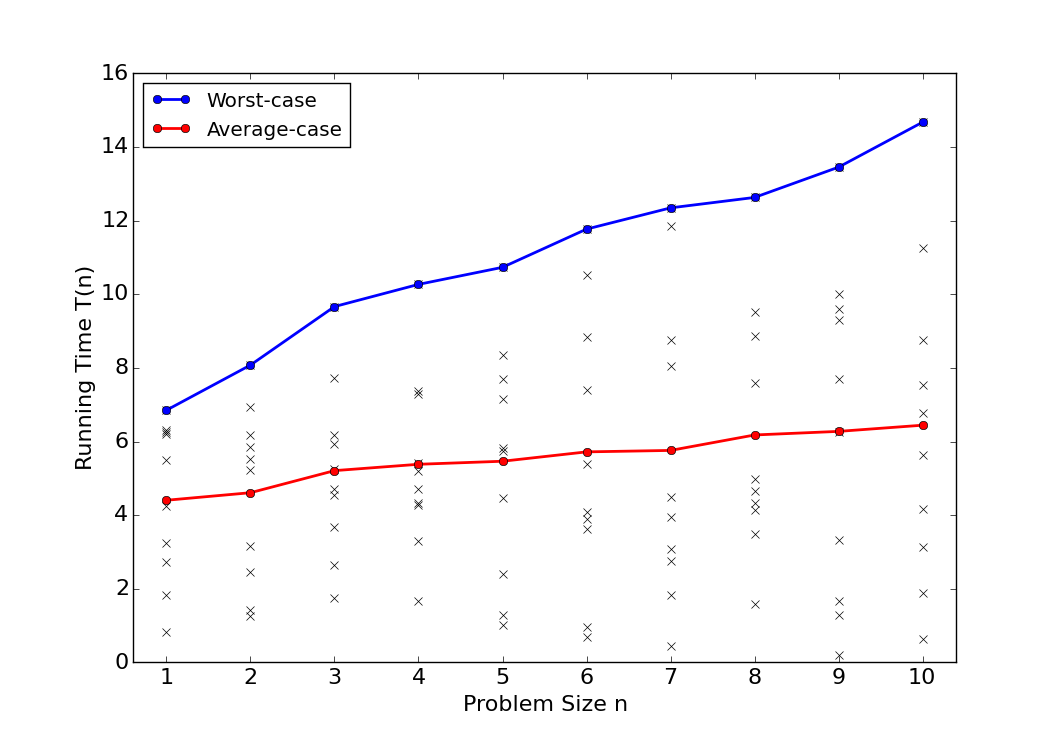
\includegraphics[width=3in] {WorstAverageCase.png}
\end{figure}
\begin{itemize}
	\item Worst-case: the case that takes the longest time; 
	\item Average-case: we need know the distribution of the instances; 
\end{itemize}
	
}



\end{document}
